\chapter{Quantification of Spatial Self-Shielding Effects}
\label{chap:quantify}


%%%%%%%%%%%%%%%%%%%%%%%%%%%%%%%%%%%%%%%%%%%%%%%%%%%%%%%%%%%%%%%%%%%%%%%%%%%%%%%
\section{Overview}
\label{sec:chap8-overview}

The preceding chapter introduced six heterogeneous 2D \ac{PWR} benchmarks derived from the \ac{BEAVRS} model, along with reference metrics tallied by OpenMC. This chapter applies multi-group transport calculations to model the same benchmarks in OpenMOC with \ac{MGXS} generated by OpenMC. The objective is to identify the bias between OpenMC and OpenMOC for \ac{MGXS} libraries which account for spatial self-shielding effects\footnote{The effects of neighboring pins, burnable poisons, reflectors and the core baffle, barrel and vessel are all of interest in the context of spatial self-shielding in this and subsequent chapters.} to varying degrees. In particular, this chapter quantifies the difference in the approximation error between simulations in which the same \ac{MGXS} are used in each unique fuel pin (\textit{e.g.}, each fuel enrichment) and those in which unique \ac{MGXS} are used in each and every pin. The former case does little if anything to model spatial self-shielding effects, whereas the latter case ``fully'' resolves these effects, albeit at the expense of very large \ac{MGXS} libraries. This difference in approximation error motivates the development of a novel methodology in the following chapters which uses statistical clustering to capture spatial self-shielding effects in \ac{MGXS}.

Three different schemes for spatial homogenization of pin-wise \ac{MGXS} are introduced in Sec.~\ref{sec:chap8-pinwise-space-homogenize} and are referred to as \textit{infinite}, \textit{null} and \textit{degenerate} spatial homogenization, respectively. The discretized models and runtime parameters used in the OpenMOC simulations are detailed in Sec.~\ref{sec:chap8-moc-params}. The bias between the OpenMOC simulations and the reference OpenMC results -- including eigenvalues, pin-wise fission rates and pin-wise U-238 capture rates -- are presented in Sec.~\ref{sec:chap8-mg-results}. The need for a new, more flexible and specialized approach to spatial homogenization which appropriately captures spatial self-shielding effects with minimal computational expense is discussed in Sec.~\ref{sec:chap8-motivate}.


%%%%%%%%%%%%%%%%%%%%%%%%%%%%%%%%%%%%%%%%%%%%%%%%%%%%%%%%%%%%%%%%%%%%%%%%%%%%%%%
\section{Pin-wise Spatial Homogenization Schemes}
\label{sec:chap8-pinwise-space-homogenize}

This chapter employs three different spatial homogenization schemes to model spatial self-shielding effects in \ac{MGXS}. Although all spatial zones may experience spatial self-shielding, this chapter only models the impact of spatial self-shielding on \ac{MGXS} in fissile regions. The infinite, null and degenerate spatial homogenization schemes are introduced in Secs.~\Crefrange{subsec:chap8-infinite}{subsec:chap8-degenerate}. These schemes model spatial self-shielding for each fuel pin with increasing granularity and complexity. The total number of materials (\textit{i.e.}, \ac{MGXS}) used to model each benchmark with each homogenization scheme is given in Tab.~\ref{table:chap8-num-materials}. A fuel assembly, 2$\times$2 colorset and part of the quarter core \ac{BEAVRS} model are color-coded by material and illustrated in Fig.~\ref{fig:chap8-homogenization-schemes} for each homogenization scheme.

The \texttt{openmc.mgxs} module (see Sec.~\ref{subsec:chap4-mgxs}) was used to compute 70-group \ac{MGXS} with OpenMC for each of the six heterogeneous benchmarks introduced in Chap.~\ref{chap:benchmarks}. The tallied \ac{MGXS} data was condensed to coarse 2-group and 8-group structures with downstream data processing as necessary. The OpenMC simulations were performed with 1000 batches with 10$^{6}$ particle histories per batch for each benchmark. This was only one tenth of the 10$^7$ histories per batch used to tally the reference results in Chap.~\ref{chap:benchmarks} for practical computational reasons\footnote{The total runtime consumed by OpenMC scales with the number of tallied quantities. The number of tallies used to compute \ac{MGXS} was much larger than the three used to compute the reference solutions in Chap.~\ref{chap:benchmarks}. As a result, the simulation time per history was prohibitively slow to generate \ac{MGXS} with the same number of histories as was used to compute the reference solution.}. The fission source was converged with 200 inactive batches for the quarter core \ac{BEAVRS} model, while 100 inactive batches were employed for the other five benchmarks (see Sec.~\ref{subsec:chap7-src-stationarity}). OpenMC's ``iso-in-lab'' feature (see Sec.~\ref{subsec:chap4-iso-in-lab}) was employed to enable consistent comparisons between OpenMC's reference results and OpenMOC's calculations with an isotropic in lab scattering source.

\vspace{0.2in}

\begin{table}[h!]
  \centering
  \caption[Number of materials for each spatial homogenization scheme]{Number of materials modeled with unique \ac{MGXS} in each heterogeneous benchmark for each spatial homogenization scheme.}
  \small
  \label{table:chap8-num-materials}
  \vspace{6pt}
  \begin{tabular}{l r r r}
  \toprule
  \rowcolor{lightgray}
  & \multicolumn{3}{c}{\cellcolor{lightgray} \bf \# Fuel Materials} \\
  \multirow{-2}{*}{\cellcolor{lightgray} \bf Benchmark} &
  \multicolumn{1}{c}{\cellcolor{lightgray} \bf Infinite} &
  \multicolumn{1}{c}{\cellcolor{lightgray} \bf Null} &
  \multicolumn{1}{c}{\cellcolor{lightgray} \bf Degenerate} \\
  \midrule
1.6\% Assm & 1 & 1 & 264 \\
%1.6\% Assm & 5 & 5 & 268 \\
  \midrule
3.1\% Assm & 1 & 1 & 264 \\
%3.1\% Assm & 5 & 5 & 268 \\
  \midrule
3.1\% Assm w/ 20 BPs & 1 & 1 & 264  \\
%3.1\% Assm w/ 20 BPs & 7 & 7 & 270  \\
  \midrule
2$\times$2 Colorset & 2 & 2 & 1,056 \\
%2$\times$2 Colorset & 8 & 8 & 1,062 \\
  \midrule
2$\times$2 Colorset w/ Reflector & 2 & 2 & 1,056 \\
%2$\times$2 Colorset w/ Reflector & 8 & 8 & 1,062 \\
  \midrule
\ac{BEAVRS} Quarter Core & 3 & 3 & 12,993 \\ % 193 * 264 / 4. + 128 + 127 + 7 % 50,964
%\ac{BEAVRS} Quarter Core & 10 & 10 & 13,000 \\ % 193 * 264 / 4. + 128 + 127 + 7 % 50,964
  \bottomrule
\end{tabular}
\end{table}

\begin{figure}[h!]
\centering
\begin{subfigure}{.45\textwidth}
  \centering
  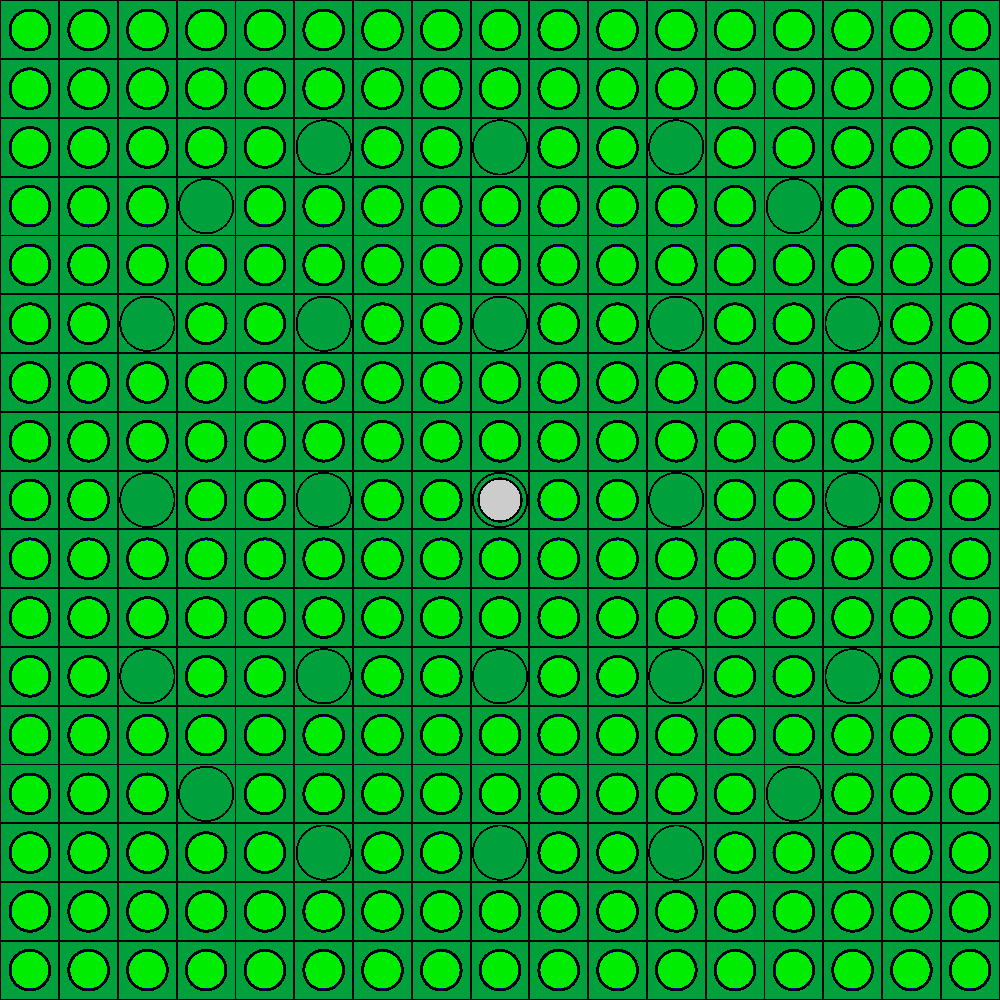
\includegraphics[width=0.87\linewidth]{figures/quantification/homogenization/assm-16-null-materials}
  \caption{}
  \label{fig:chap8-assm-16-null-materials}
\end{subfigure}%
\begin{subfigure}{.45\textwidth}
  \centering
  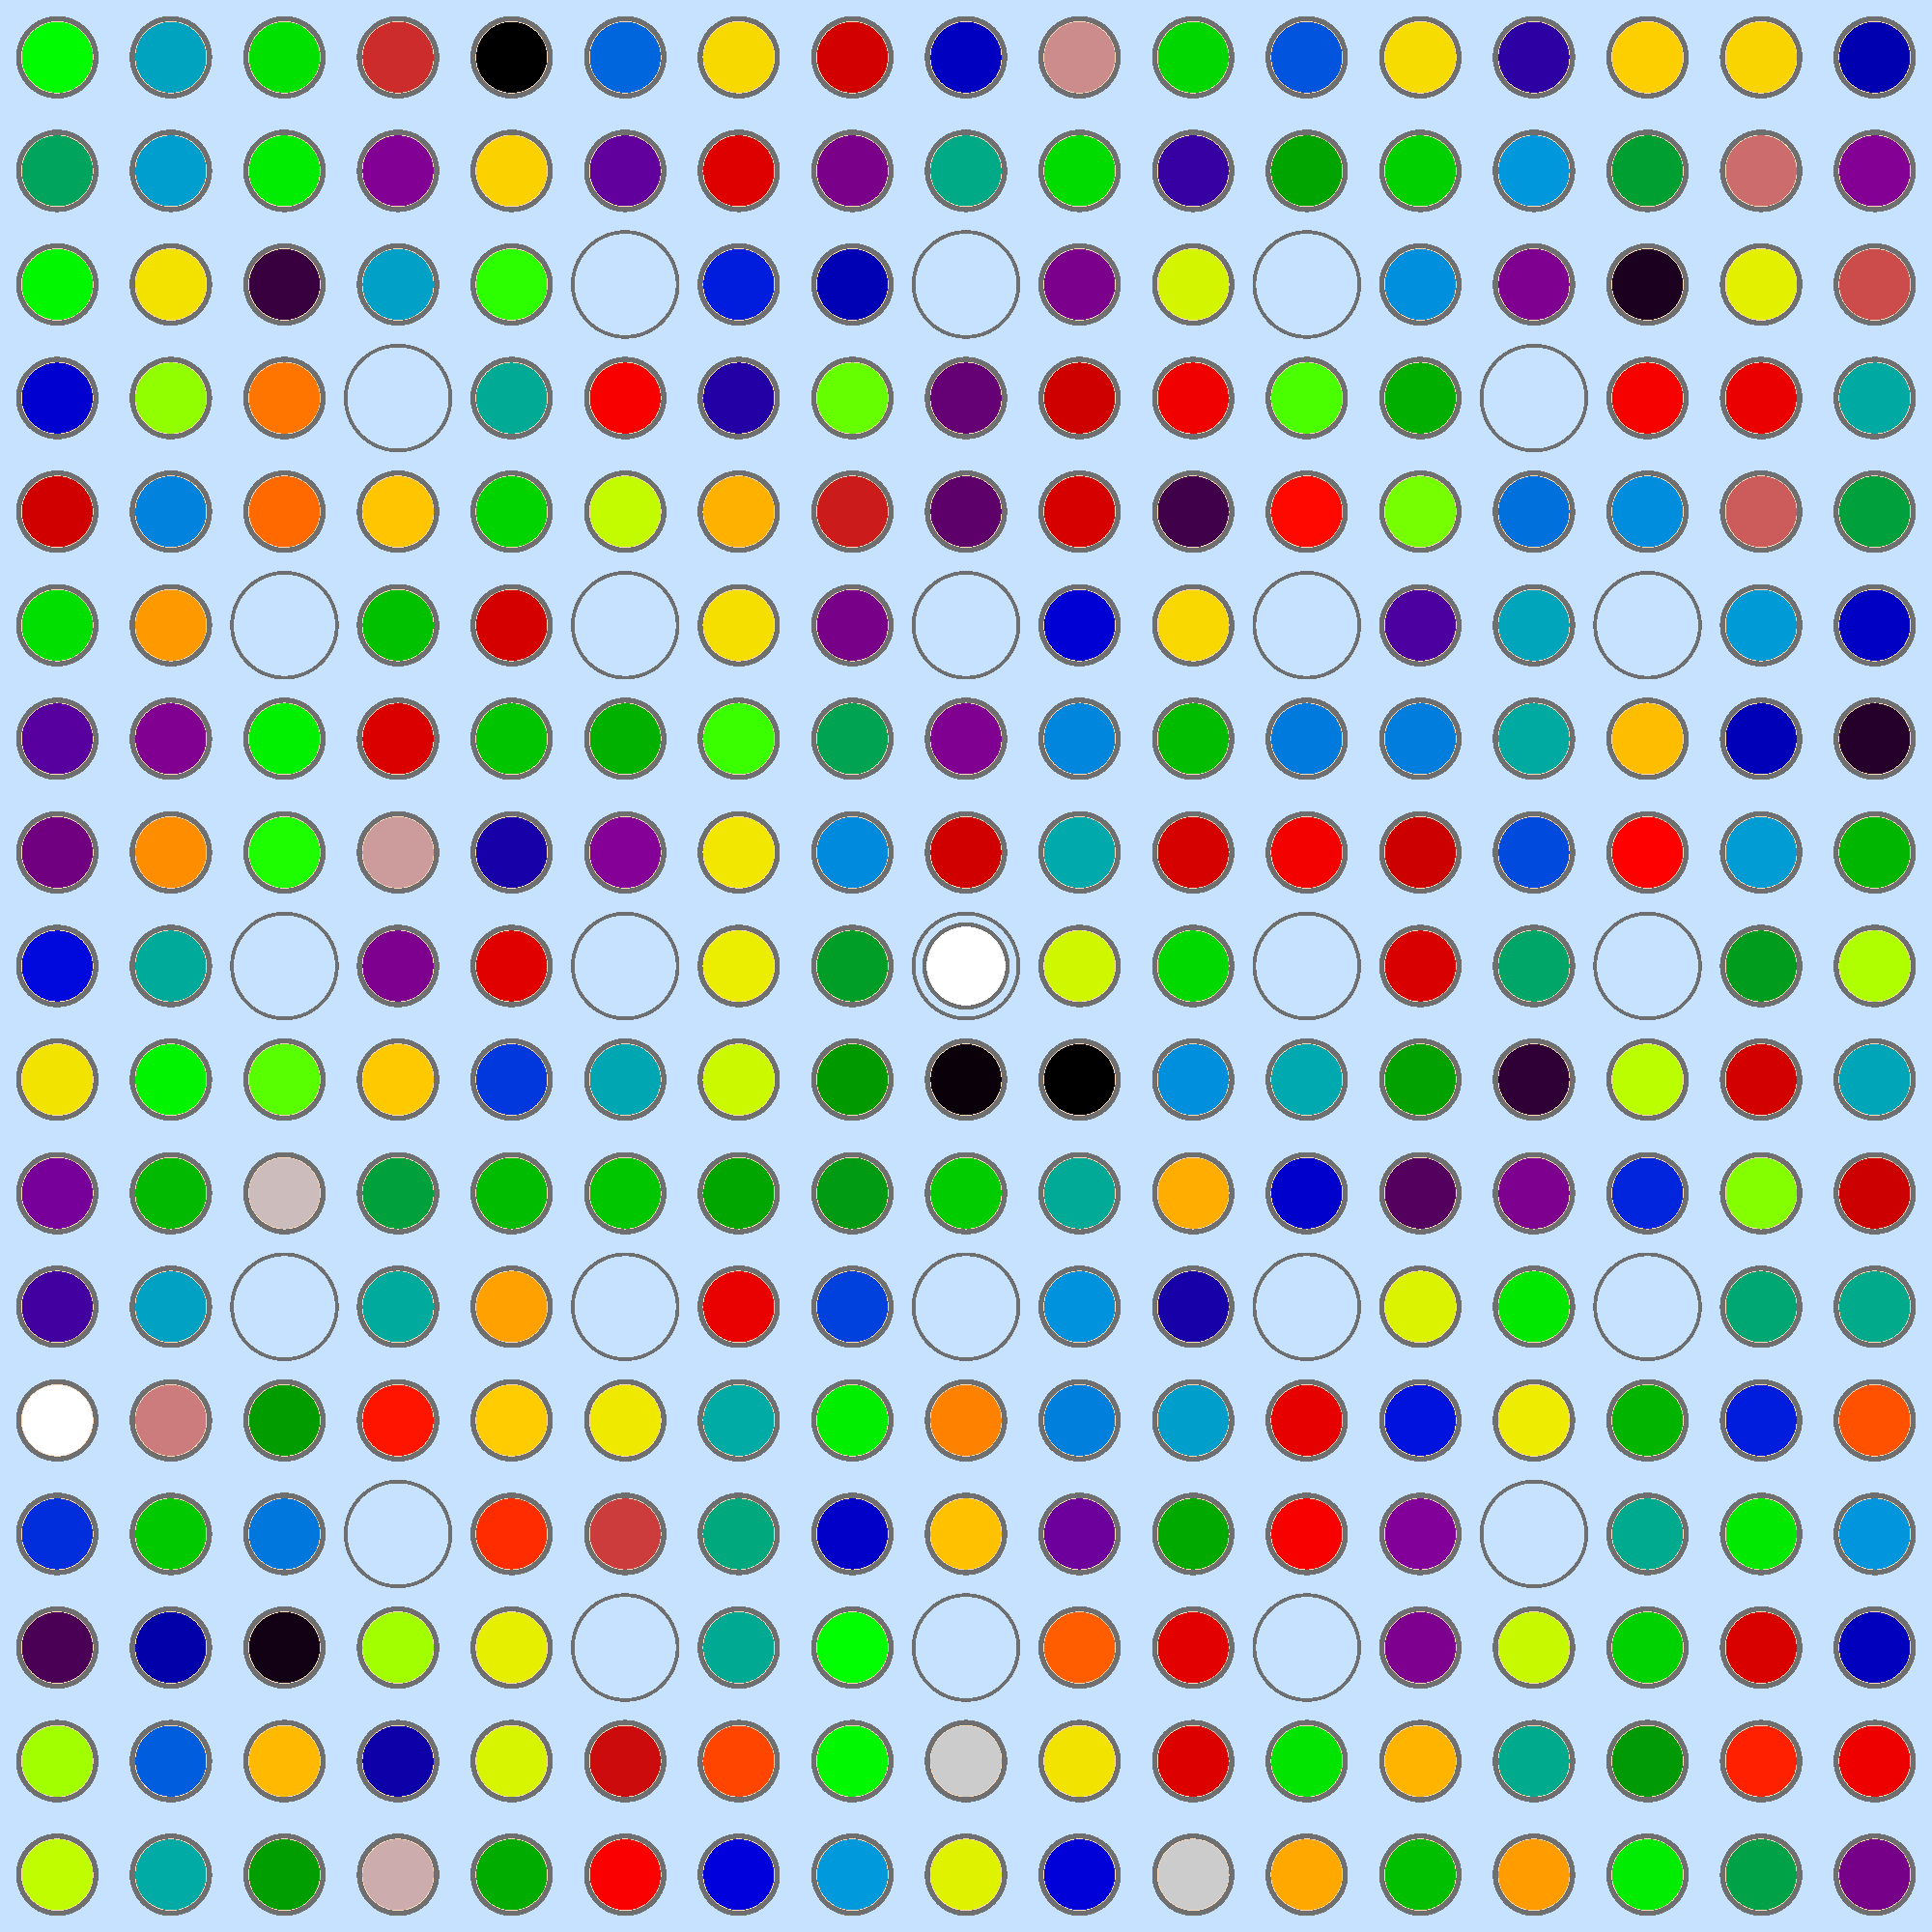
\includegraphics[width=0.87\linewidth]{figures/quantification/homogenization/assm-16-degenerate-materials}
  \caption{}
  \label{fig:chap8-assm-16-degenerate-materials}
\end{subfigure}
\begin{subfigure}{.45\textwidth}
  \centering
  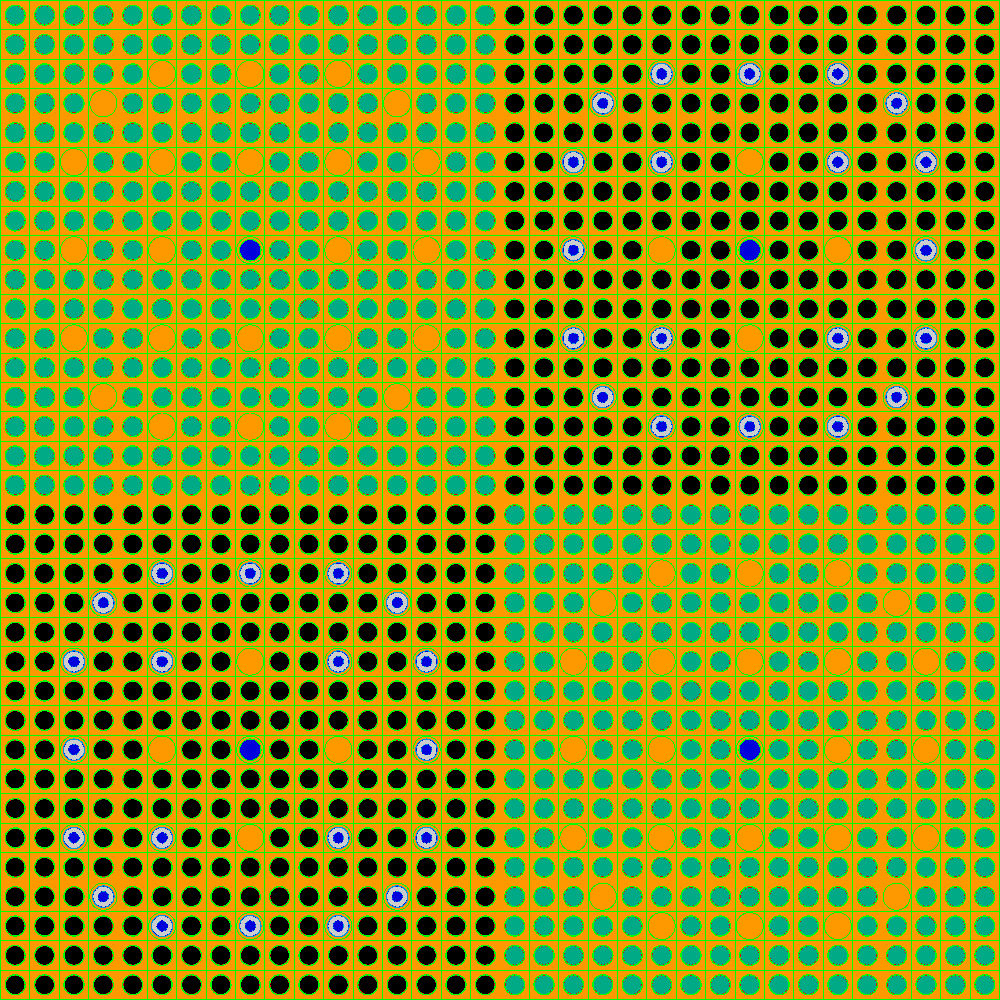
\includegraphics[width=0.87\linewidth]{figures/quantification/homogenization/2x2-null-materials}
  \caption{}
  \label{fig:chap8-2x2-null-materials}
\end{subfigure}%
\begin{subfigure}{.45\textwidth}
  \centering
  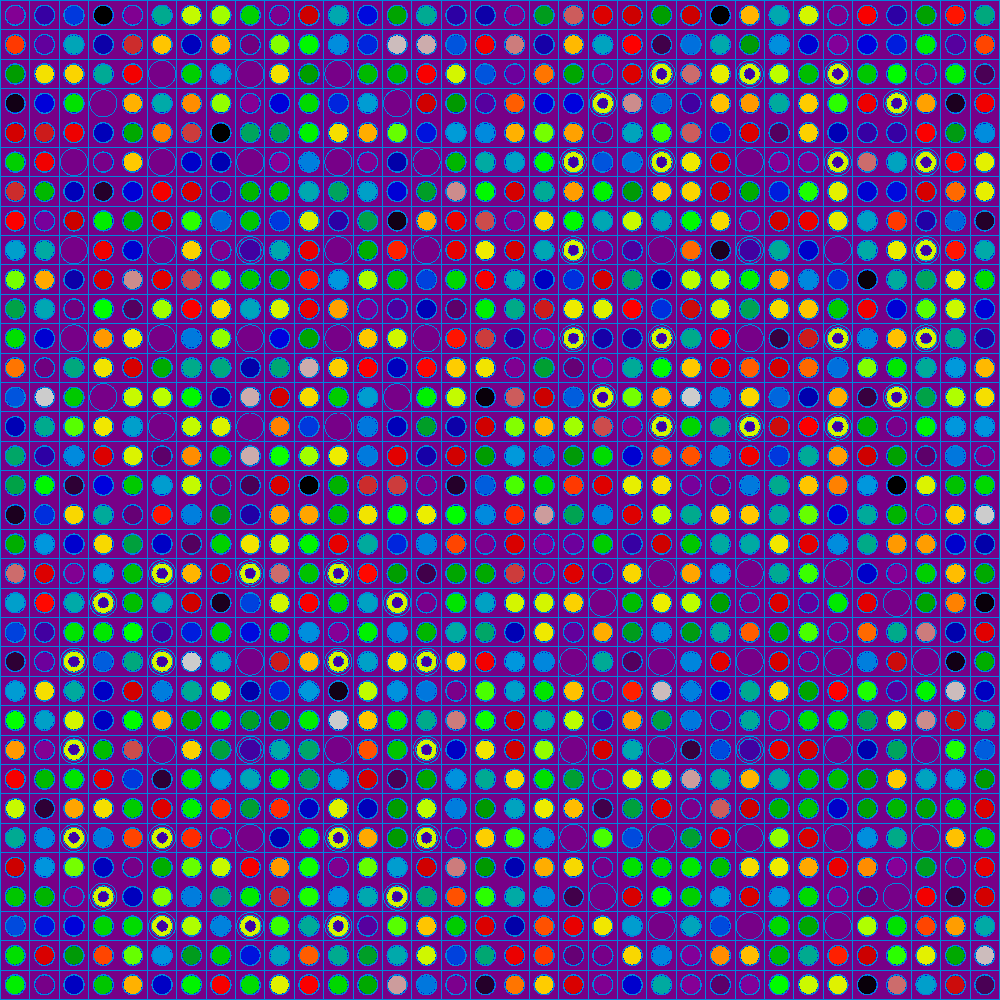
\includegraphics[width=0.87\linewidth]{figures/quantification/homogenization/2x2-degenerate-materials}
  \caption{}
  \label{fig:chap8-2x2-degenerate-materials}
\end{subfigure}
\begin{subfigure}{.45\textwidth}
  \centering
  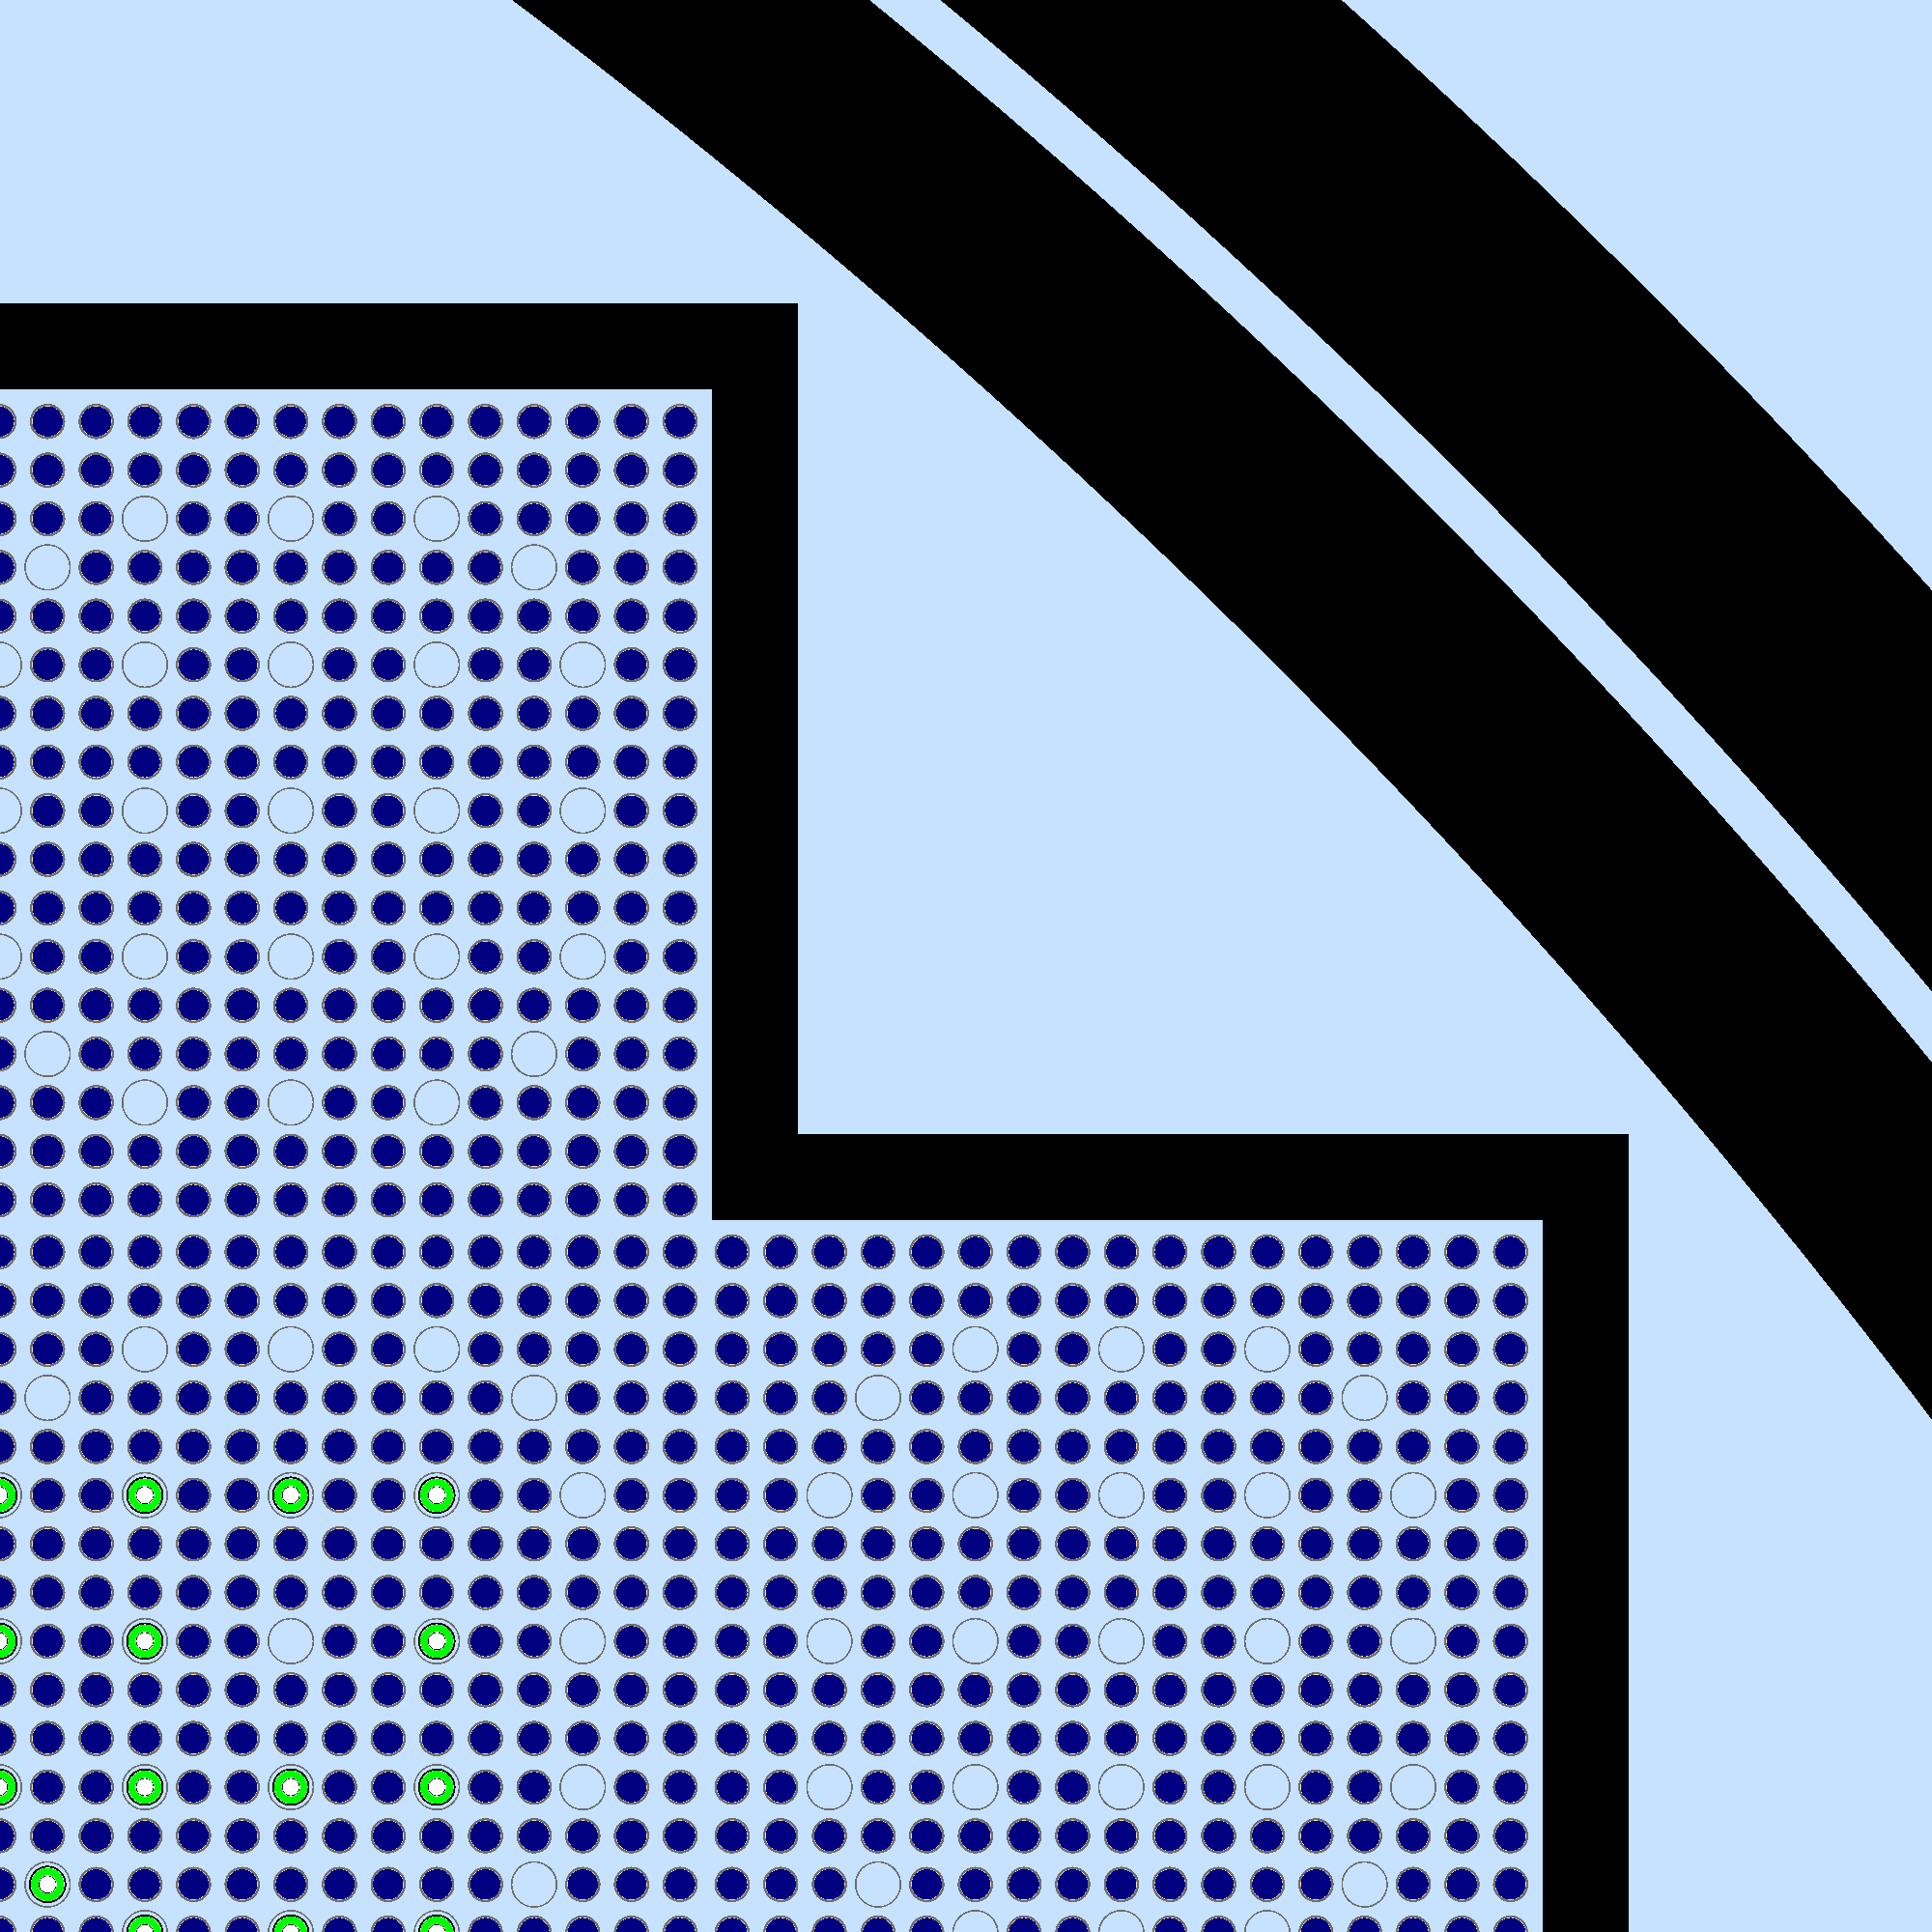
\includegraphics[width=0.87\linewidth]{figures/quantification/homogenization/full-core-null-materials}
  \caption{}
  \label{fig:chap8-full-core-null-materials}
\end{subfigure}%
\begin{subfigure}{.45\textwidth}
  \centering
  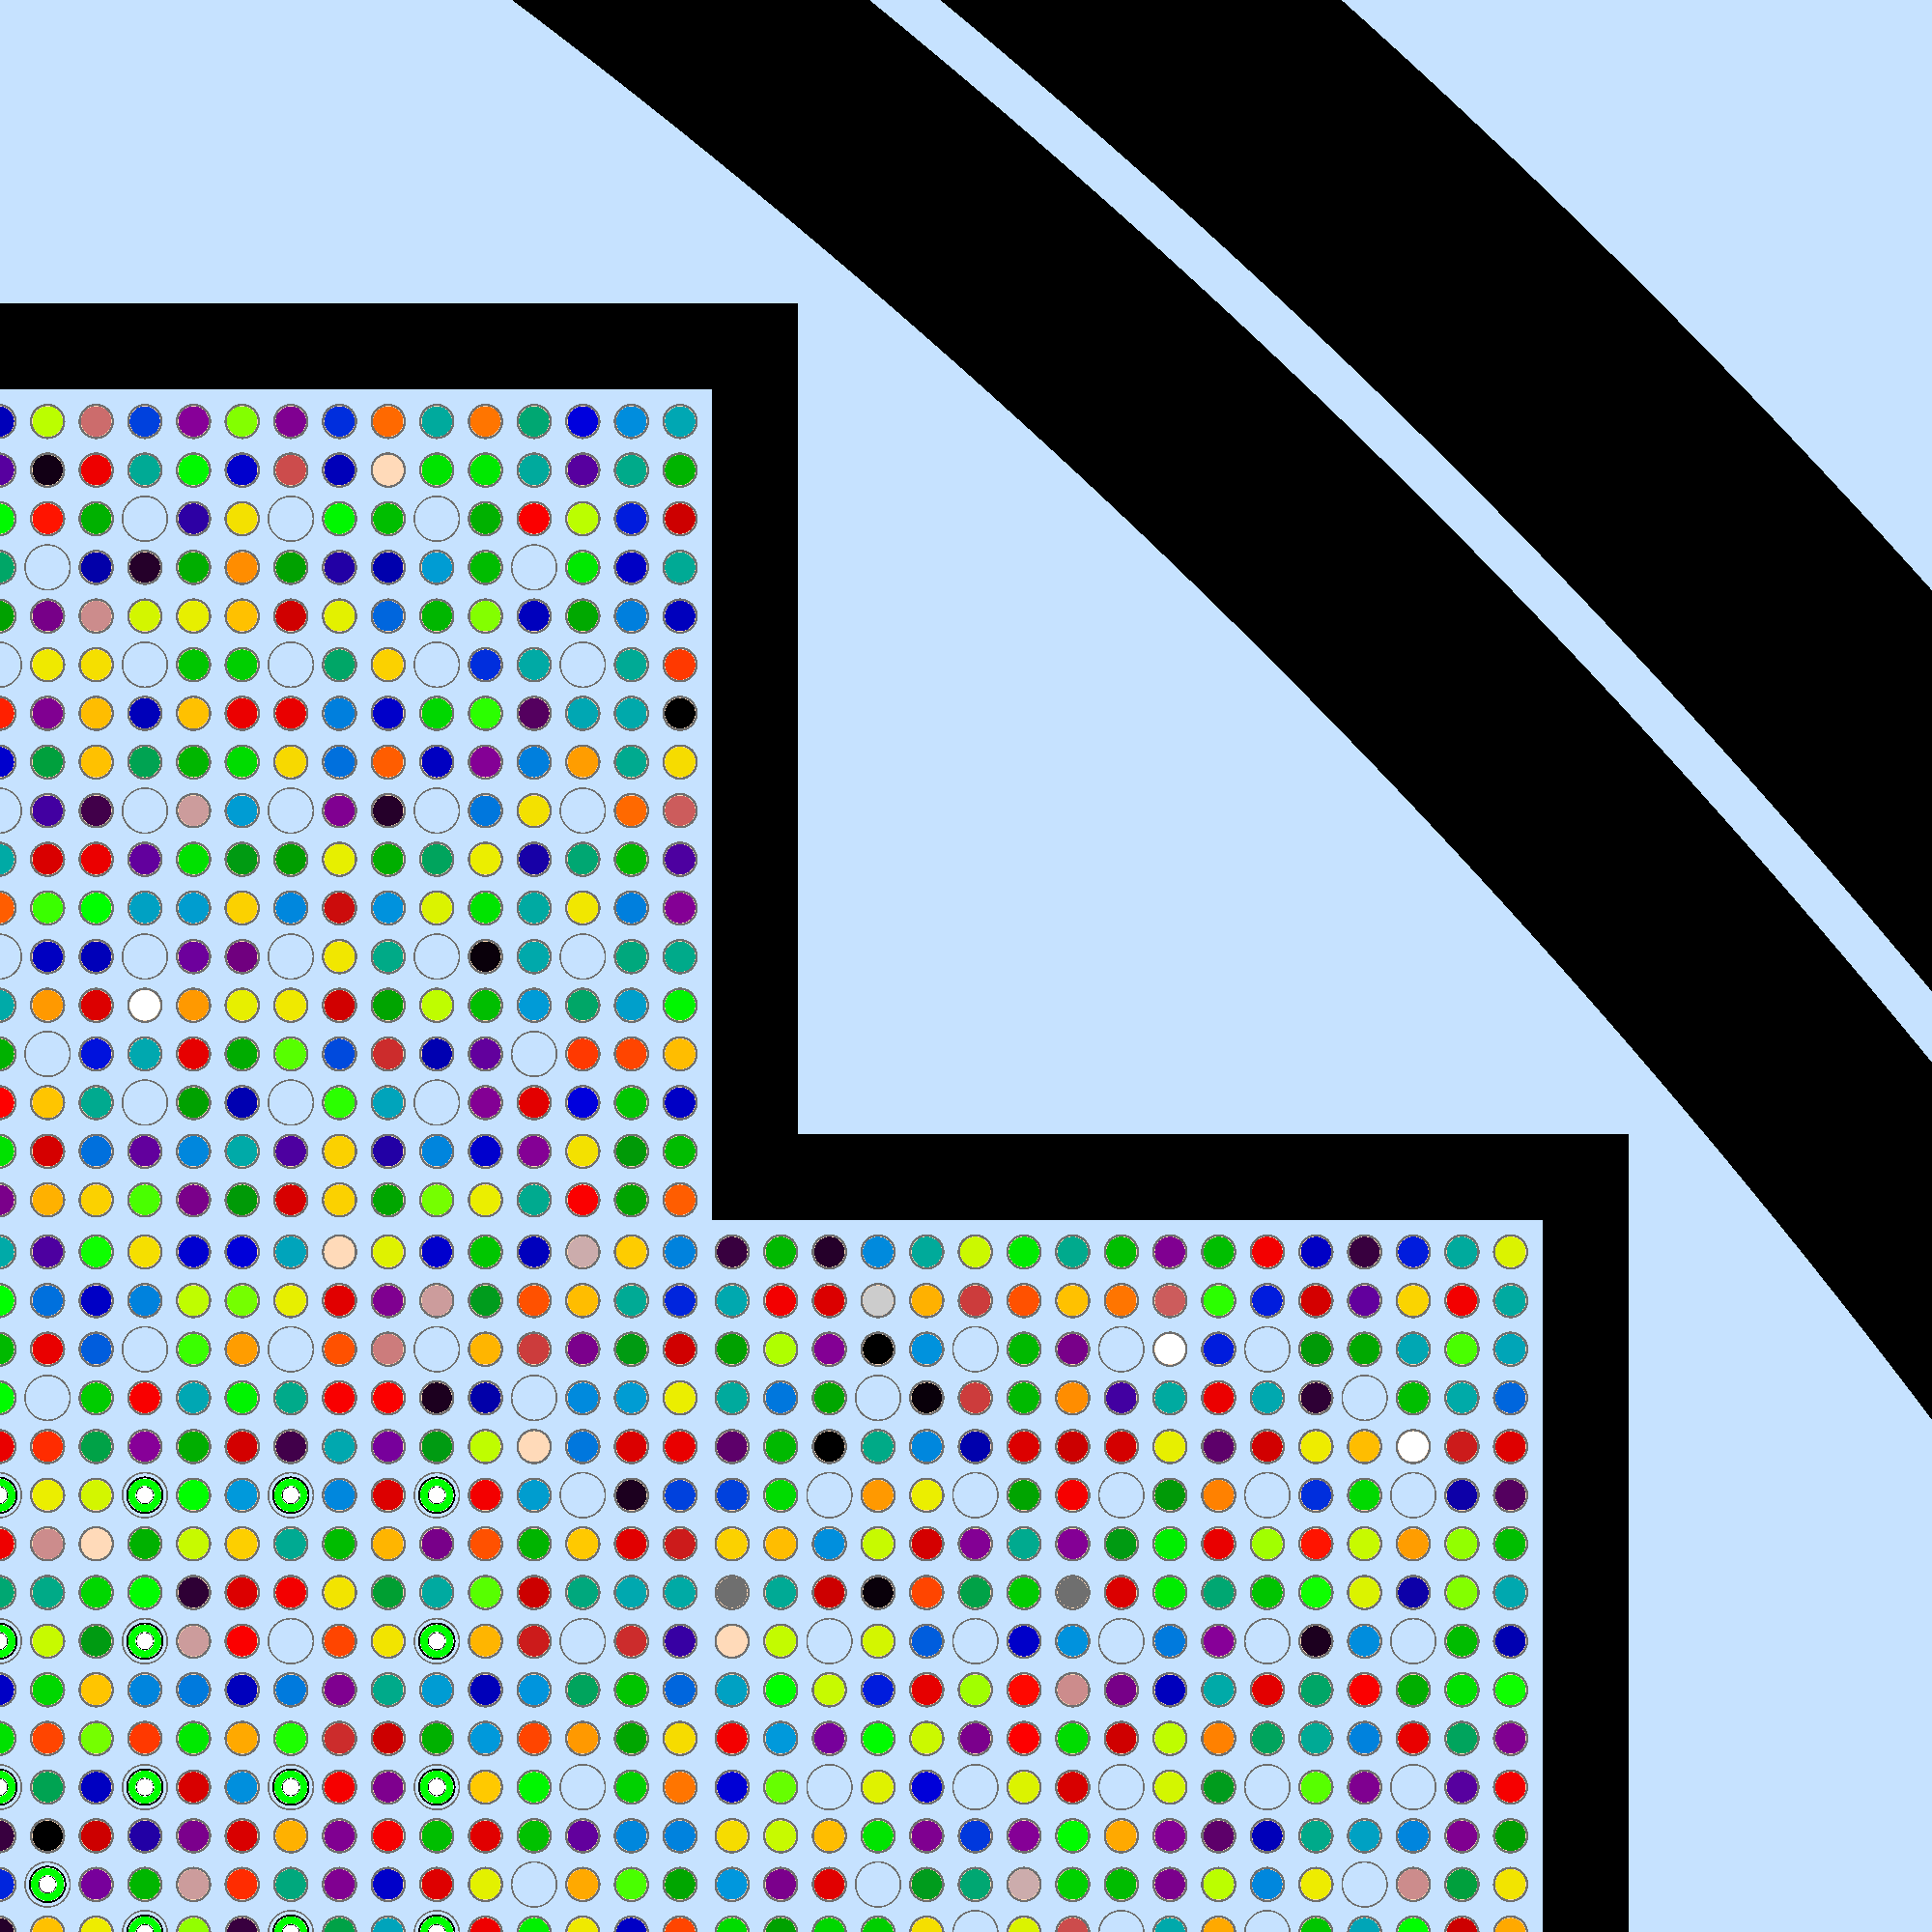
\includegraphics[width=0.87\linewidth]{figures/quantification/homogenization/full-core-degenerate-materials}
  \caption{}
  \label{fig:chap8-full-core-degenerate-materials}
\end{subfigure}
\caption[Depiction of infinite, null and degenerate spatial homogenization schemes]{OpenMOC materials for a single fuel assembly, a 2$\times$2 colorset and part of the 2D quarter core \ac{BEAVRS} model. The materials for the infinite and null schemes are depicted in (a), (c) and (e), and for the degenerate scheme in (b), (d) and (f), respectively. Each uniquely colored material represents a unique set of \ac{MGXS}.}
\label{fig:chap8-homogenization-schemes}
\end{figure}

%%%%%%%%%%%%%%%%%%%%%%%%%%%%%%%%%%%%%%
\subsection{Infinite Lattice Homogenization}
\label{subsec:chap8-infinite}

The \textit{infinite} spatial homogenization scheme is most reminiscent of the traditional multi-level schemes used to generate \ac{MGXS} (see Sec.~\ref{subsec:chap2-mgxs-lib-std-approach}), and is the simplest approach to model spatial self-shielding effects considered by this thesis. The infinite scheme employs multiple OpenMC simulations to compute \ac{MGXS} for each heterogeneous benchmark. The \ac{MGXS} for each type of fuel (\textit{e.g.}, enrichment) are generated by OpenMC simulations of each fuel pin type in an infinite, repeating array\footnote{An infinite, repeating array of fuel pins is modeled by a single fuel pin with reflective boundary conditions.}. The \ac{MGXS} for all other materials -- including borated water, zircaloy, helium, etc. -- are generated from OpenMC simulations of each heterogeneous benchmark where the reaction rates and fluxes are averaged across each geometry.

The infinite scheme is designed to quantify the impact of using the ``true'' Monte Carlo flux from an infinite lattice calculation, rather than the ``true'' \ac{MC} flux from the true heterogeneous geometry, to collapse \ac{MGXS} in fissile zones. The scheme employs a single \ac{MGXS} in each instance of a material zone, such as a fuel pin replicated many times throughout a benchmark geometry. The \ac{MGXS} for each fissile zone is generated from an infinite lattice calculation with OpenMC. The \ac{MGXS} for all non-fissile zones are generated using the ``true''  flux distribution in space and energy for each of the heterogeneous benchmarks. The scheme does not account for spatial self-shielding effects experienced by different non-fissile spatial zones filled by the same material, and instead averages these effects across the entire geometry for each material.

%-foonote: unable to run infinite pin cell calculations for non-fissile pin cells (CRGTs, BPs, instr tubes) since it's not a criticality calculation

%%%%%%%%%%%%%%%%%%%%%%%%%%%%%%%%%%%%%%
\subsection{Null Homogenization}
\label{subsec:chap8-null}

The \textit{null} spatial homogenization scheme builds upon the infinite scheme, but uses the ``true'' heterogeneous flux to collapse \ac{MGXS} for fissile as well as non-fissile materials. The null scheme eliminates the infinite lattice calculation to generate \ac{MGXS} for fissile zones, and instead uses a single Monte Carlo calculation of the complete heterogeneous geometry to generate \ac{MGXS} for \textit{all} materials. In this way, the null scheme fully abandons the multi-level approach used by the infinite scheme and most traditional approaches to generate \ac{MGXS}. Unlike the infinite scheme, the spatially self-shielded flux is used to collapse the cross sections in the fuel. However, the null scheme does not account for spatial self-shielding effects experienced by different fuel pins filled by the same type of fuel, and instead averages these effects across the entire geometry. As with the infinite scheme, a single \ac{MGXS} is employed in each instance of a material zone, such as a fuel pin replicated many times throughout a benchmark geometry.

%%%%%%%%%%%%%%%%%%%%%%%%%%%%%%%%%%%%%%
\subsection{Degenerate Homogenization}
\label{subsec:chap8-degenerate}

Unlike the infinite and null spatial homogenization schemes, the \textit{degenerate} scheme accounts for the different spatial self-shielding effects experienced by each instance of each fuel pin throughout a heterogeneous geometry. Like the null scheme, a single \ac{MC} calculation of the complete heterogeneous geometry is used to generate \ac{MGXS} for all materials. Unlike the null scheme, the \ac{MGXS} are tallied separately for each instance of fissile material zones. For example, if a heterogeneous benchmark includes $N$ fuel pins, then $N$ collections of \ac{MGXS} are separately tabulated for each fuel pin instance. The degenerate scheme tallies different \ac{MGXS} even if the isotopic compositions in the fuel pin instances are identical (\textit{e.g.}, fresh fuel at the beginning of life) since each instance may experience different spatial self-shielding effects and hence have different \ac{MGXS}.

Multi-group transport calculations with \ac{MGXS} generated using infinite/null and degenerate schemes may be compared to quantify the impact of modeling spatial self-shielding effects in \ac{MGXS} for fissile zones in heterogeneous geometries. The degenerate scheme applies the finest granularity to pin-wise spatial homogenization of any of the schemes considered in this thesis since it best captures different spatial self-shielding effects in each fuel pin. As a result, the degenerate scheme is used to benchmark the efficacy of the new methodology for spatial homogenization based on statistical clustering developed in the following chapters. Like both the infinite and null schemes, the spatial self-shielding effects experienced by different non-fissile spatial zones are averaged across the entire geometry for each non-fissile material.

The degenerate scheme generates \ac{MGXS} for each fuel pin instance using OpenMC's distributed cell tallies (see Sec.~\ref{subsec:chap4-distribcells}). The OpenCG region differentiation algorithm (see Sec.~\ref{sec:chap4-region-diff}) is used to build a new OpenMOC geometry with unique cells and materials for each fuel pin. The \ac{MGXS} are appropriately selected from OpenMC's distributed cell tallies to populate the \ac{MGXS} in the OpenMOC materials.

\begin{emphbox}
\textbf{The infinite, null and degenerate spatial homogenization schemes are used to quantify approximation errors made when neglecting spatial self-shielding due to neighboring pins, reflectors, etc. in heterogeneous \ac{PWR} benchmarks.}
\end{emphbox}


%%%%%%%%%%%%%%%%%%%%%%%%%%%%%%%%%%%%%%%%%%%%%%%%%%%%%%%%%%%%%%%%%%%%%%%%%%%%%%%
\section{\ac{MOC} Runtime Parameters}
\label{sec:chap8-moc-params}

The infinite, null and spatial homogenization schemes were used to prepare \ac{MGXS} libraries for OpenMOC simulations of each of the six heterogeneous \ac{PWR} benchmarks introduced in Chap.~\ref{chap:benchmarks}. This section briefly outlines the energy group structures and angular, spatial and \ac{CMFD} meshes used in the OpenMOC simulations. The total number of flat source regions, and \ac{MOC} tracks and segments are summarized for each benchmark in Tab.~\ref{table:chap8-num-fsrs-tracks-segments}. It was crucial to use an adequate discretization to accurately compare simulation results between the three spatial homogenization schemes, as well as to the reference OpenMC results.

\begin{table}[h!]
  \centering
  \caption[Number of \ac{FSR}s, tracks and segments for each heterogeneous benchmark]{The number of \ac{MOC} \ac{FSR}s, tracks and segments modeled in each benchmark.}
  \small
  \label{table:chap8-num-fsrs-tracks-segments}
  \vspace{6pt}
  \begin{tabular}{l r r r}
  \toprule
  \rowcolor{lightgray}
  \textbf{Benchmark} &
  \multicolumn{1}{c}{\cellcolor{lightgray} \textbf{\# \ac{FSR}s}} &
  \multicolumn{1}{c}{\cellcolor{lightgray} \textbf{\# Tracks}} &
  \multicolumn{1}{c}{\cellcolor{lightgray} \textbf{\# Segments}} \\
  \midrule
1.6\% Assm & 28,376 & 34,976 & 7,945,952 \\
  \midrule
3.1\% Assm & 28,376 & 34,976 & 7,945,952 \\
  \midrule
3.1\% Assm w/ 20 BPs & 29,496 & 34,976 & 8,110,192  \\
  \midrule
2$\times$2 Colorset & 115,744 & 69,892 & 32,097,936 \\
  \midrule
2$\times$2 Colorset w/ Reflector & 203,220 & 104,788 & 51,122,228 \\
  \midrule
%\ac{BEAVRS} Quarter Core & 2,512,384 & 201,620 & 427,683,579 \\
\ac{BEAVRS} Quarter Core & 1,718,368 & 201,620 & 38,3785,515 \\
  \bottomrule
\end{tabular}
\end{table}

Each simulation was converged to 10$^{-5}$ on the root mean square of the energy-integrated fission source in each flat source region (FSR). It should be noted that a convergence criterion of 10$^{-7}$ was employed for the OpenMOC simulations of simple benchmarks without \ac{CMFD} acceleration (see Sec.~\ref{subsubsec:chap4-openmoc-cmfd}) in Chap.~\ref{chap:biases}, but a looser convergence criterion of 10$^{-5}$ may be used for calculations with \ac{CMFD}\footnote{The convergence criterion measures the residual between successive iterations, but should actually measure convergence to the asymptotic solution, which depends on both the residual between successive iterations and the dominance ratio. \ac{CMFD} significantly reduces the residual between successive iterations such that sufficient convergence to the asymptotic solution is achieved at a much lower successive iteration residual.}.

%%%%%%%%%%%%%%%%%%%%%%%%%%%%%%%%%%%%
\subsection{Energy Group Structures}
\label{subsec:chap8-energy-groups}

Each assembly, colorset and quarter core benchmark was modeled with \ac{MGXS} in 2, 8 and 70 energy groups. The energy group structures were the same as those used in Chaps.~\ref{chap:biases} and~\ref{chap:sph} and are tabulated in App.~\ref{app:energy-groups}. The \ac{MOC} energy group structures were collapsed onto coarser group structures for \ac{CMFD} acceleration. The mapping from \ac{MOC} to \ac{CMFD} group structures is listed in Tab.~\ref{table:chap8-coarse-cmfd-groups}. The coarse \ac{CMFD} structures were derived to best approximate equal lethargy spacing between coarse \ac{CMFD} groups. The coarse \ac{CMFD} structures significantly improved the speed of the 70-group OpenMOC calculations.

\begin{table}[h!]
  \centering
  \caption[Coarse \ac{CMFD} group structures]{The coarse \ac{CMFD} group structures for each of the fine \ac{MOC} group structures.}
  \small
  \label{table:chap8-coarse-cmfd-groups}
  \vspace{6pt}
  \begin{tabular}{p{1.5cm} p{1.5cm} p{7.2cm}}
  \toprule
  \rowcolor{lightgray}
  \multicolumn{1}{c}{\cellcolor{lightgray} \textbf{\# \ac{MOC} Groups}} &
  \multicolumn{1}{c}{\cellcolor{lightgray} \textbf{\# \ac{CMFD} Groups}} &
  \multicolumn{1}{c}{\cellcolor{lightgray} \textbf{\ac{CMFD} Fine-to-Coarse Group Mapping}} \\
  \midrule
  \multicolumn{1}{c}{2} & \multicolumn{1}{c}{2} & [1], [2] \\
  \midrule
  \multicolumn{1}{c}{8} & \multicolumn{1}{c}{4} & [1--2], [3], [4--5], [6--8] \\
  \midrule
%  \multicolumn{1}{c}{40} & \multicolumn{1}{c}{10} & [1--3], [4--7], [8], [9], [10], [11--13], \hspace{0.8cm} [14--16], [17--29], [30--36], [37--40] \\
%  \midrule
  \multicolumn{1}{c}{70} & \multicolumn{1}{c}{14} & [1--2], [3--6], [7--9], [10--12], [13--16], \hspace{0.6cm} [17--19], [20--21], [22--24], [25--27], [28--33], [34--53], [54--61], [62--68], [69--70] \\ 
  \bottomrule
\end{tabular}
\end{table}

%%%%%%%%%%%%%%%%%%%%%%%%%%%%%%%%%%%%
\subsection{Angular Discretization}
\label{subsec:chap8-angular-discretizations}

The OpenMOC simulations of each of the six heterogeneous benchmarks used the same \ac{MOC} angular discretization with 128 azimuthal angles and 0.05 cm track spacing. These parameters were selected since they were previously demonstrated to converge the solution for simple heterogeneous \ac{PWR} benchmark models~\cite{boyd2014ms}. Although the eigenvalues in Chap.~\ref{chap:biases} were only shown to converge for a 1D slab and 2D fuel pin with 0.01 cm track spacing, a coarser spacing of 0.05 cm was employed for the heterogeneous benchmarks for practical reasons\footnote{The computational expense of solving the \ac{MOC} equations scales linearly with the number of track segments. In addition, OpenMOC's memory footprint is dominated by track segments which can make some problems intractable except on high memory nodes. Finally, the time spent ray tracing across a combinatorial geometry is non-negligible if not prohibitive for fine track spacings in large geometries.}. The total number of tracks and segments resulting from the selected angular discretization are itemized in Tab.~\ref{table:chap8-num-fsrs-tracks-segments}. 

%%%%%%%%%%%%%%%%%%%%%%%%%%%%%%%%%%%%
\subsection{\ac{FSR} Discretization}
\label{subsec:chap8-fsr-discretizations}

Flat source region spatial discretization meshes were applied to each of the six heterogeneous benchmarks in the OpenMOC simulations. The total number of \ac{FSR}s is itemized in Tab.~\ref{table:chap8-num-fsrs-tracks-segments} for each benchmark analyzed in this thesis. The \ac{FSR} meshes applied to the fuel pin, control rod guide tube, instrument tube and burnable poison pin cells are shown in Fig.~\ref{fig:chap8-pin-cell-fsrs}. As shown in the figures, eight equal angle subdivisions were used in all material zones. The UO$_2$ fuel was further subdivided into five equal volume radial rings, while ten radial rings were employed in the water-filled \acp{CRGT} and instrument tubes. The borosilicate glass and borated water material zones filling the \acp{BP} were each discretized into five equal volume radial rings. Finally, five equally spaced rings were used in the moderator zones surrounding each pin.

\begin{figure}[h!]
\centering
\begin{subfigure}{.5\textwidth}
  \centering
  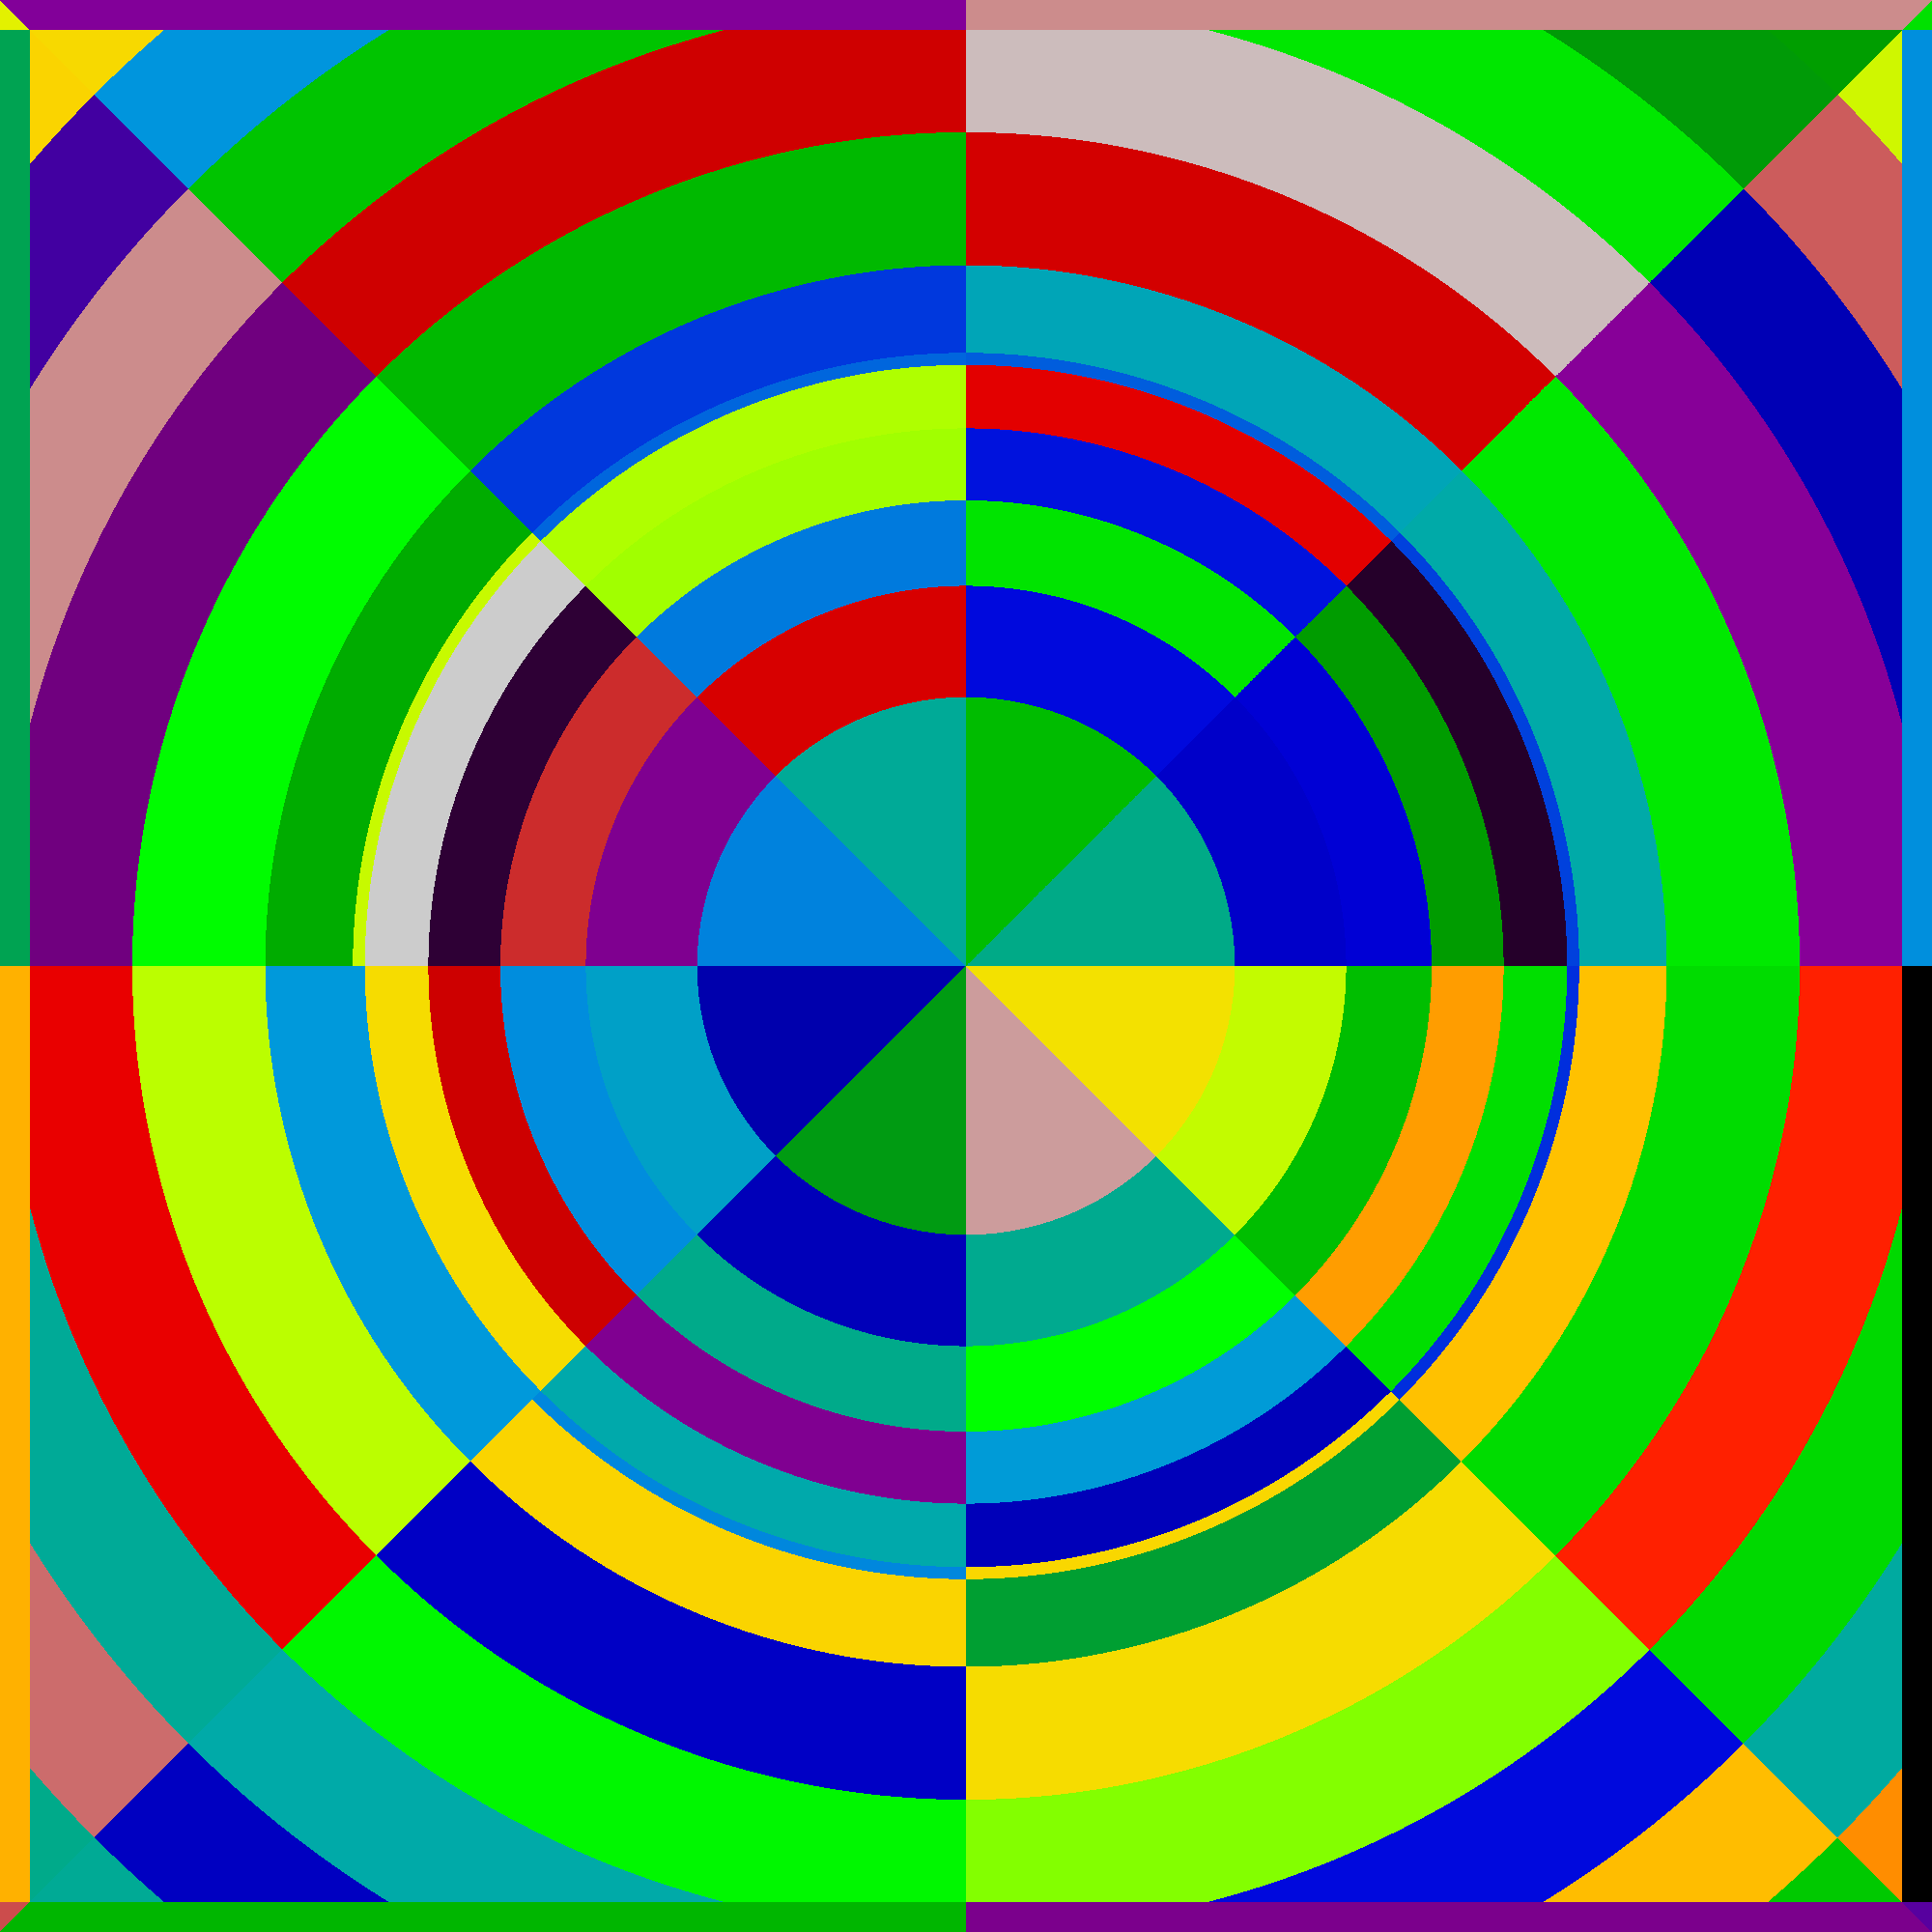
\includegraphics[width=0.8\linewidth]{figures/quantification/fsrs/fsrs-fuel-pin}
  \caption{}
  \label{fig:chap8-pin-1.6}
\end{subfigure}%
\begin{subfigure}{.5\textwidth}
  \centering
  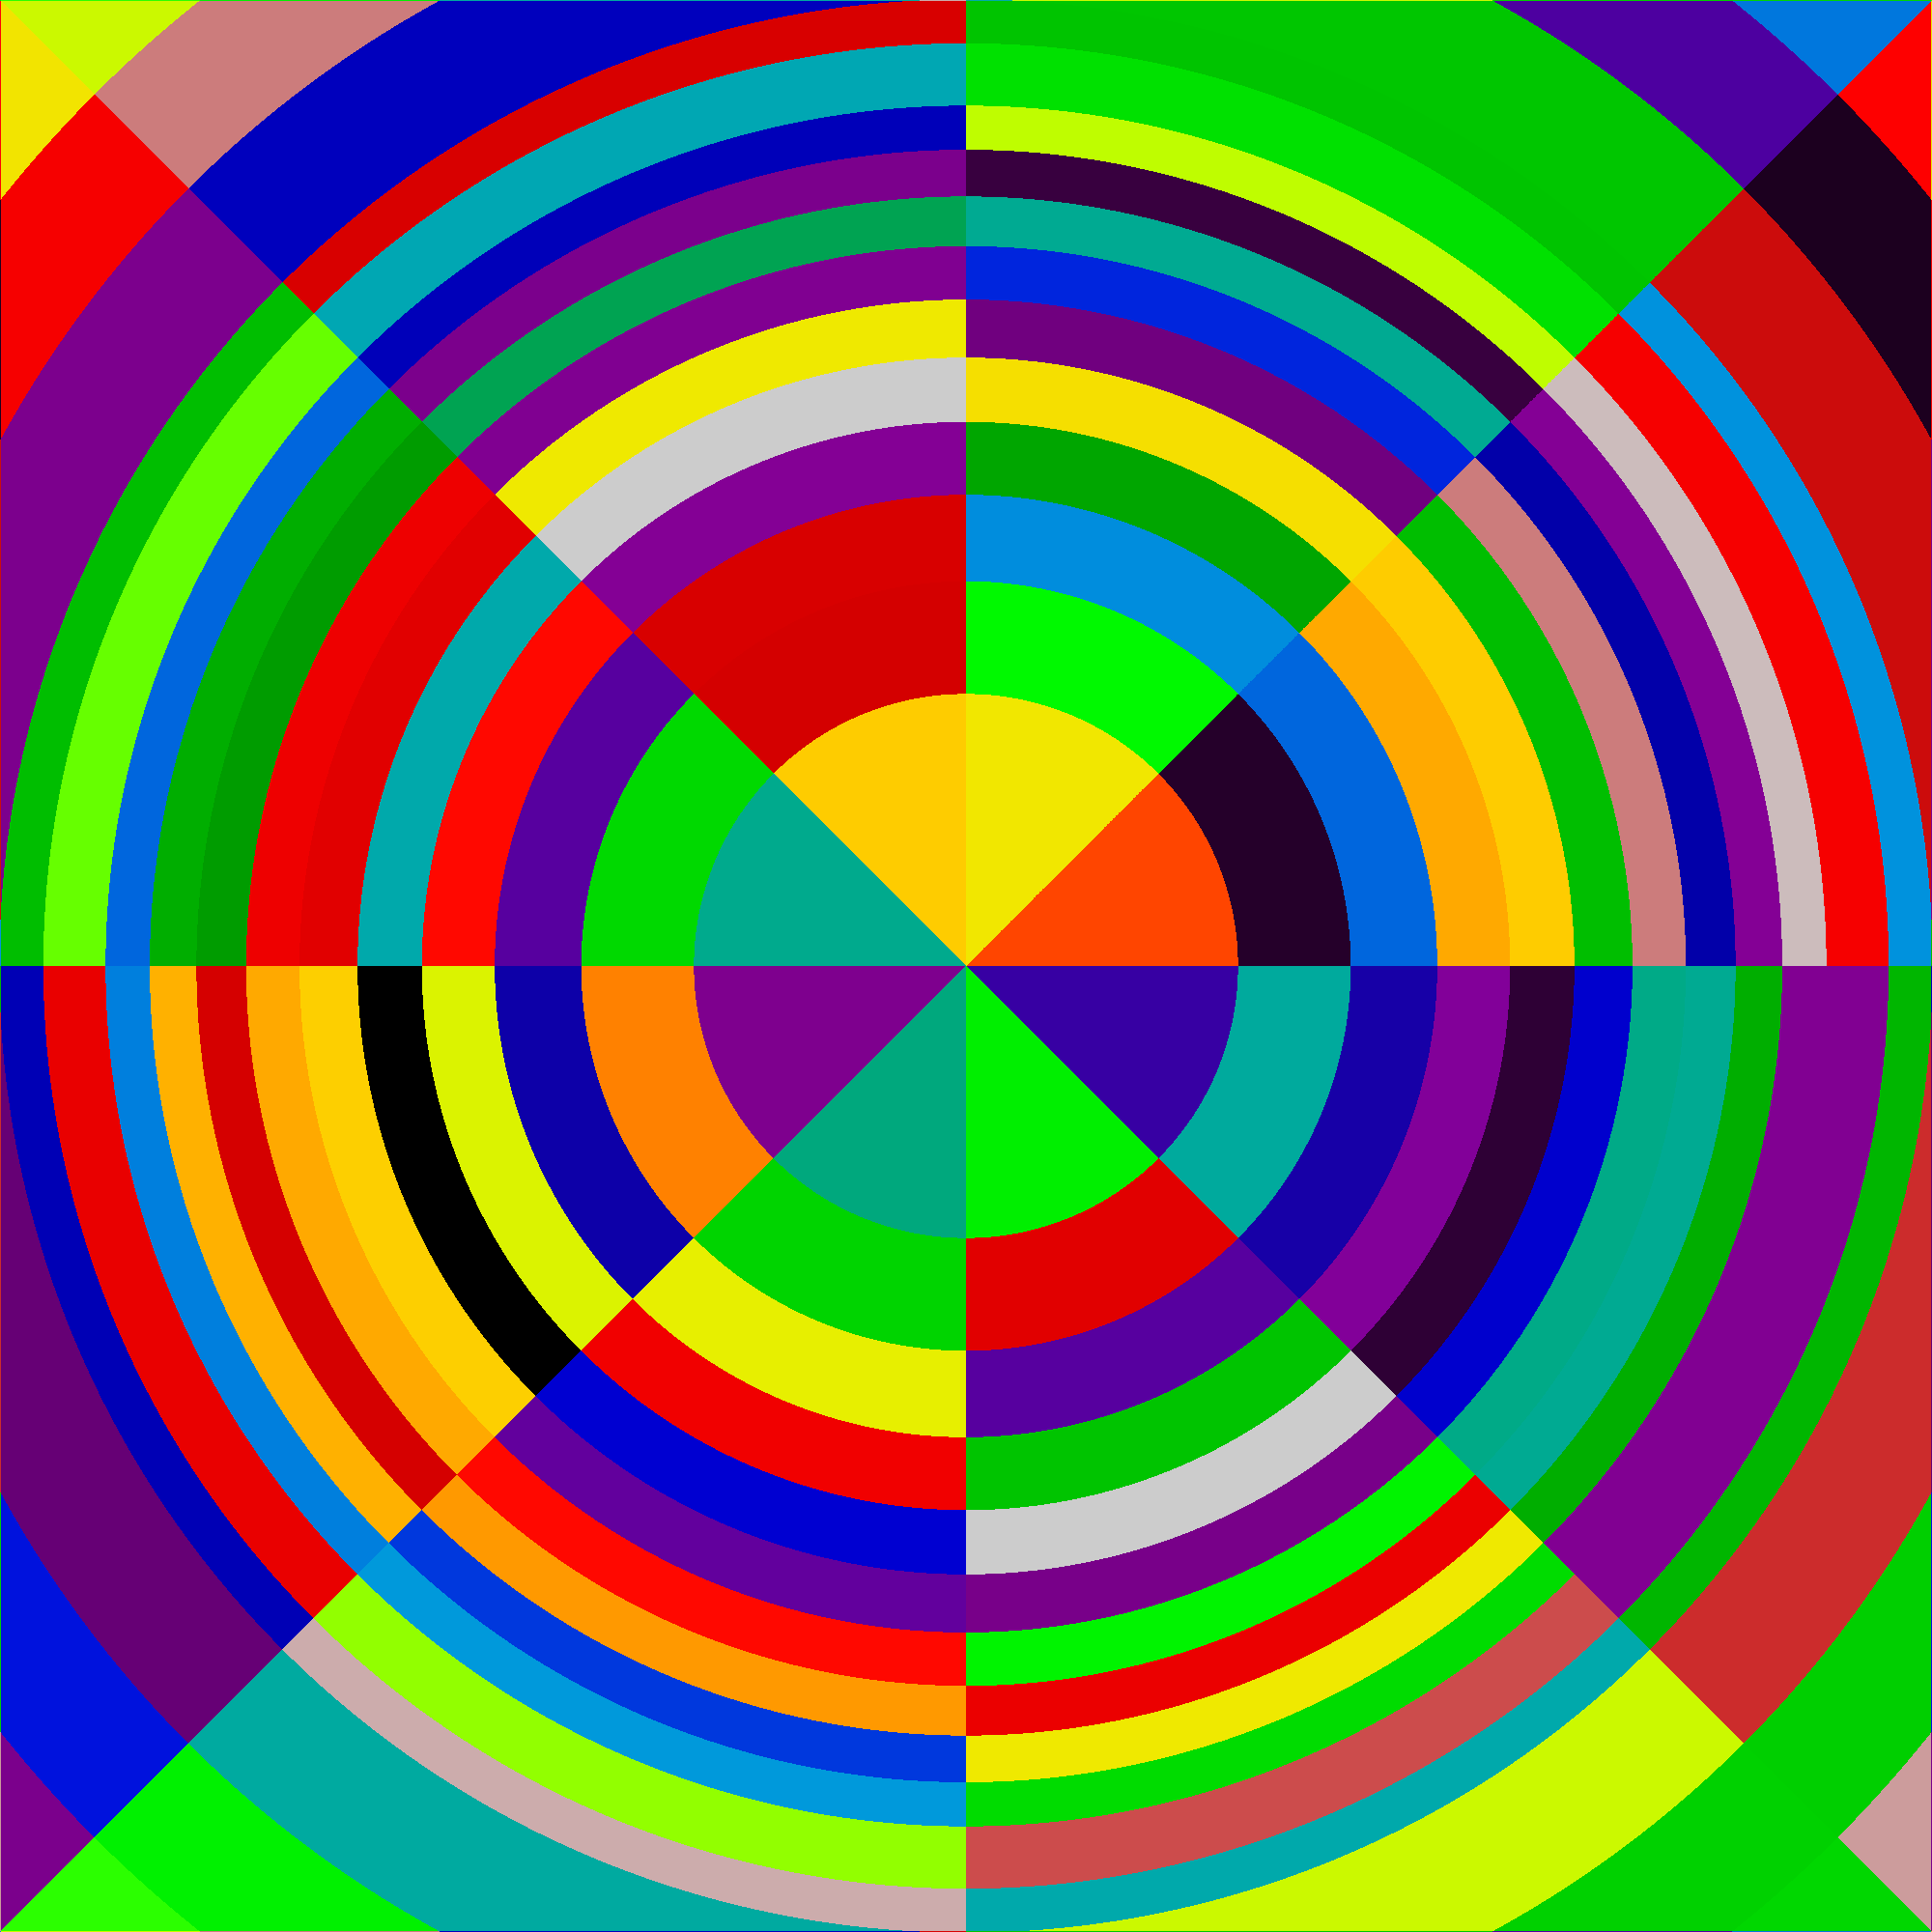
\includegraphics[width=0.8\linewidth]{figures/quantification/fsrs/fsrs-crgt}
  \caption{}
  \label{fig:chap8-pin-crgt}
\end{subfigure}
\begin{subfigure}{.5\textwidth}
  \centering
  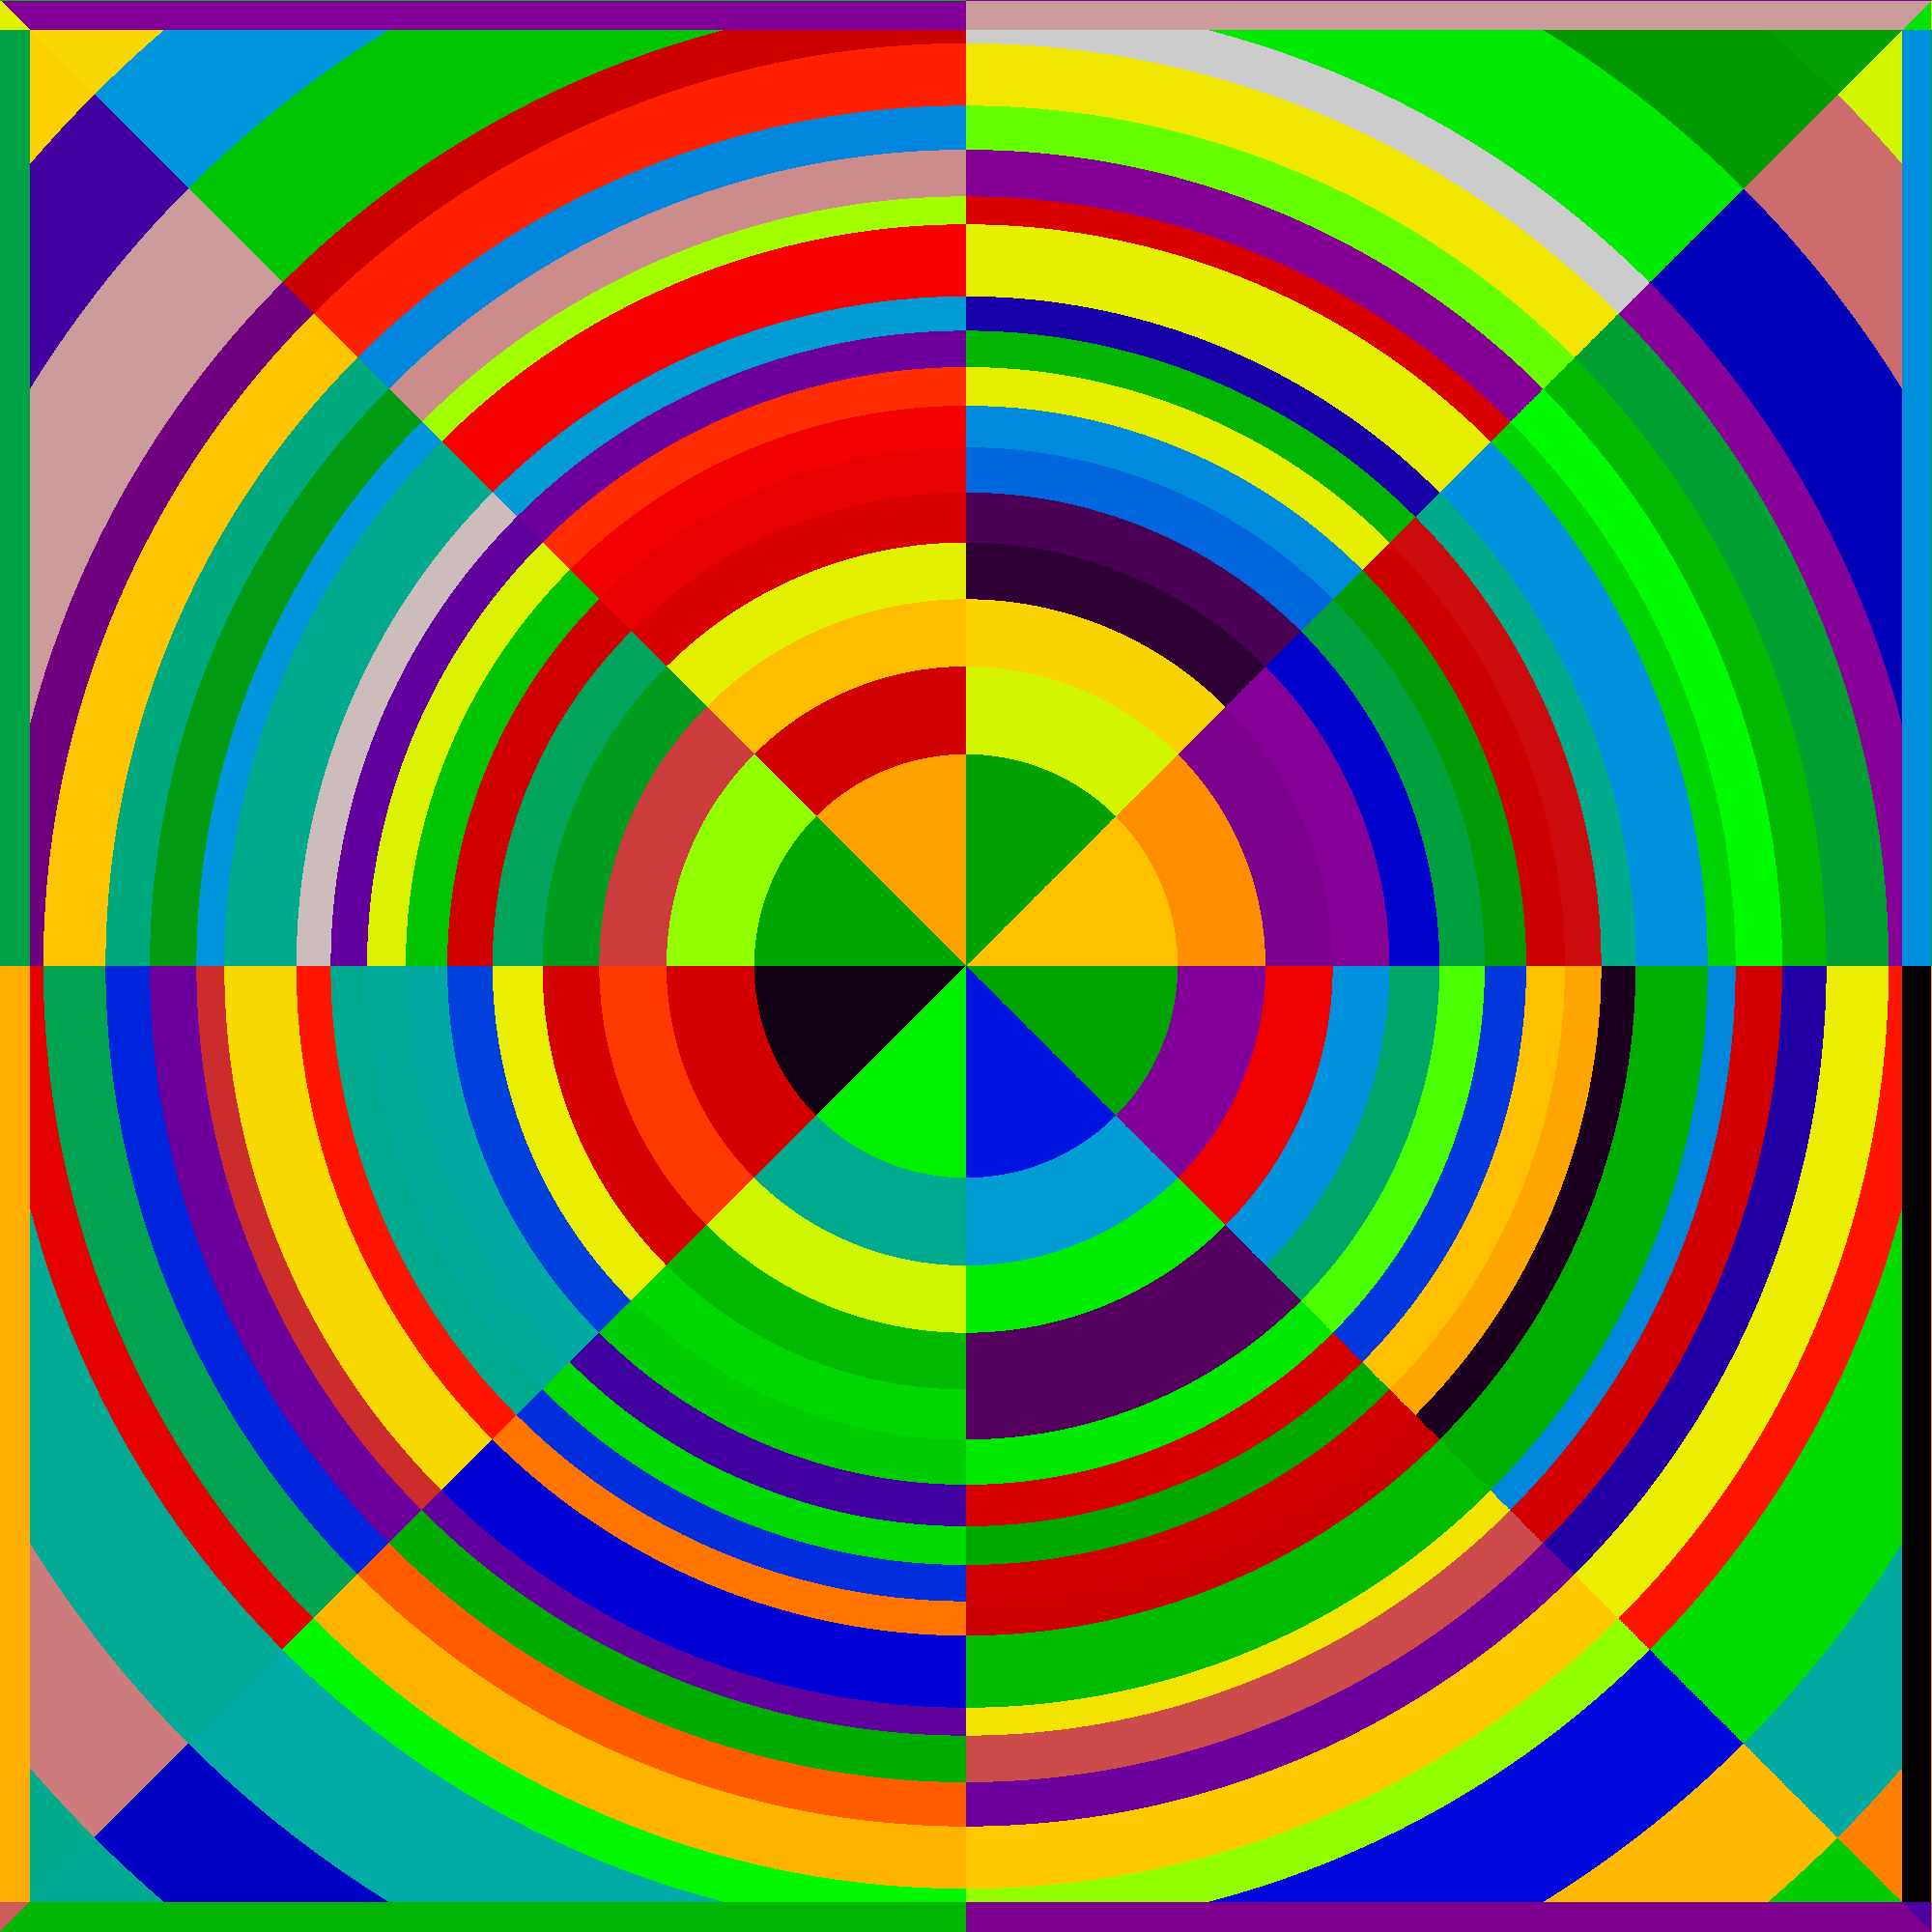
\includegraphics[width=0.8\linewidth]{figures/quantification/fsrs/fsrs-instr-tube}
  \caption{}
  \label{fig:chap8-instr-tube}
\end{subfigure}%
\begin{subfigure}{.5\textwidth}
  \centering
  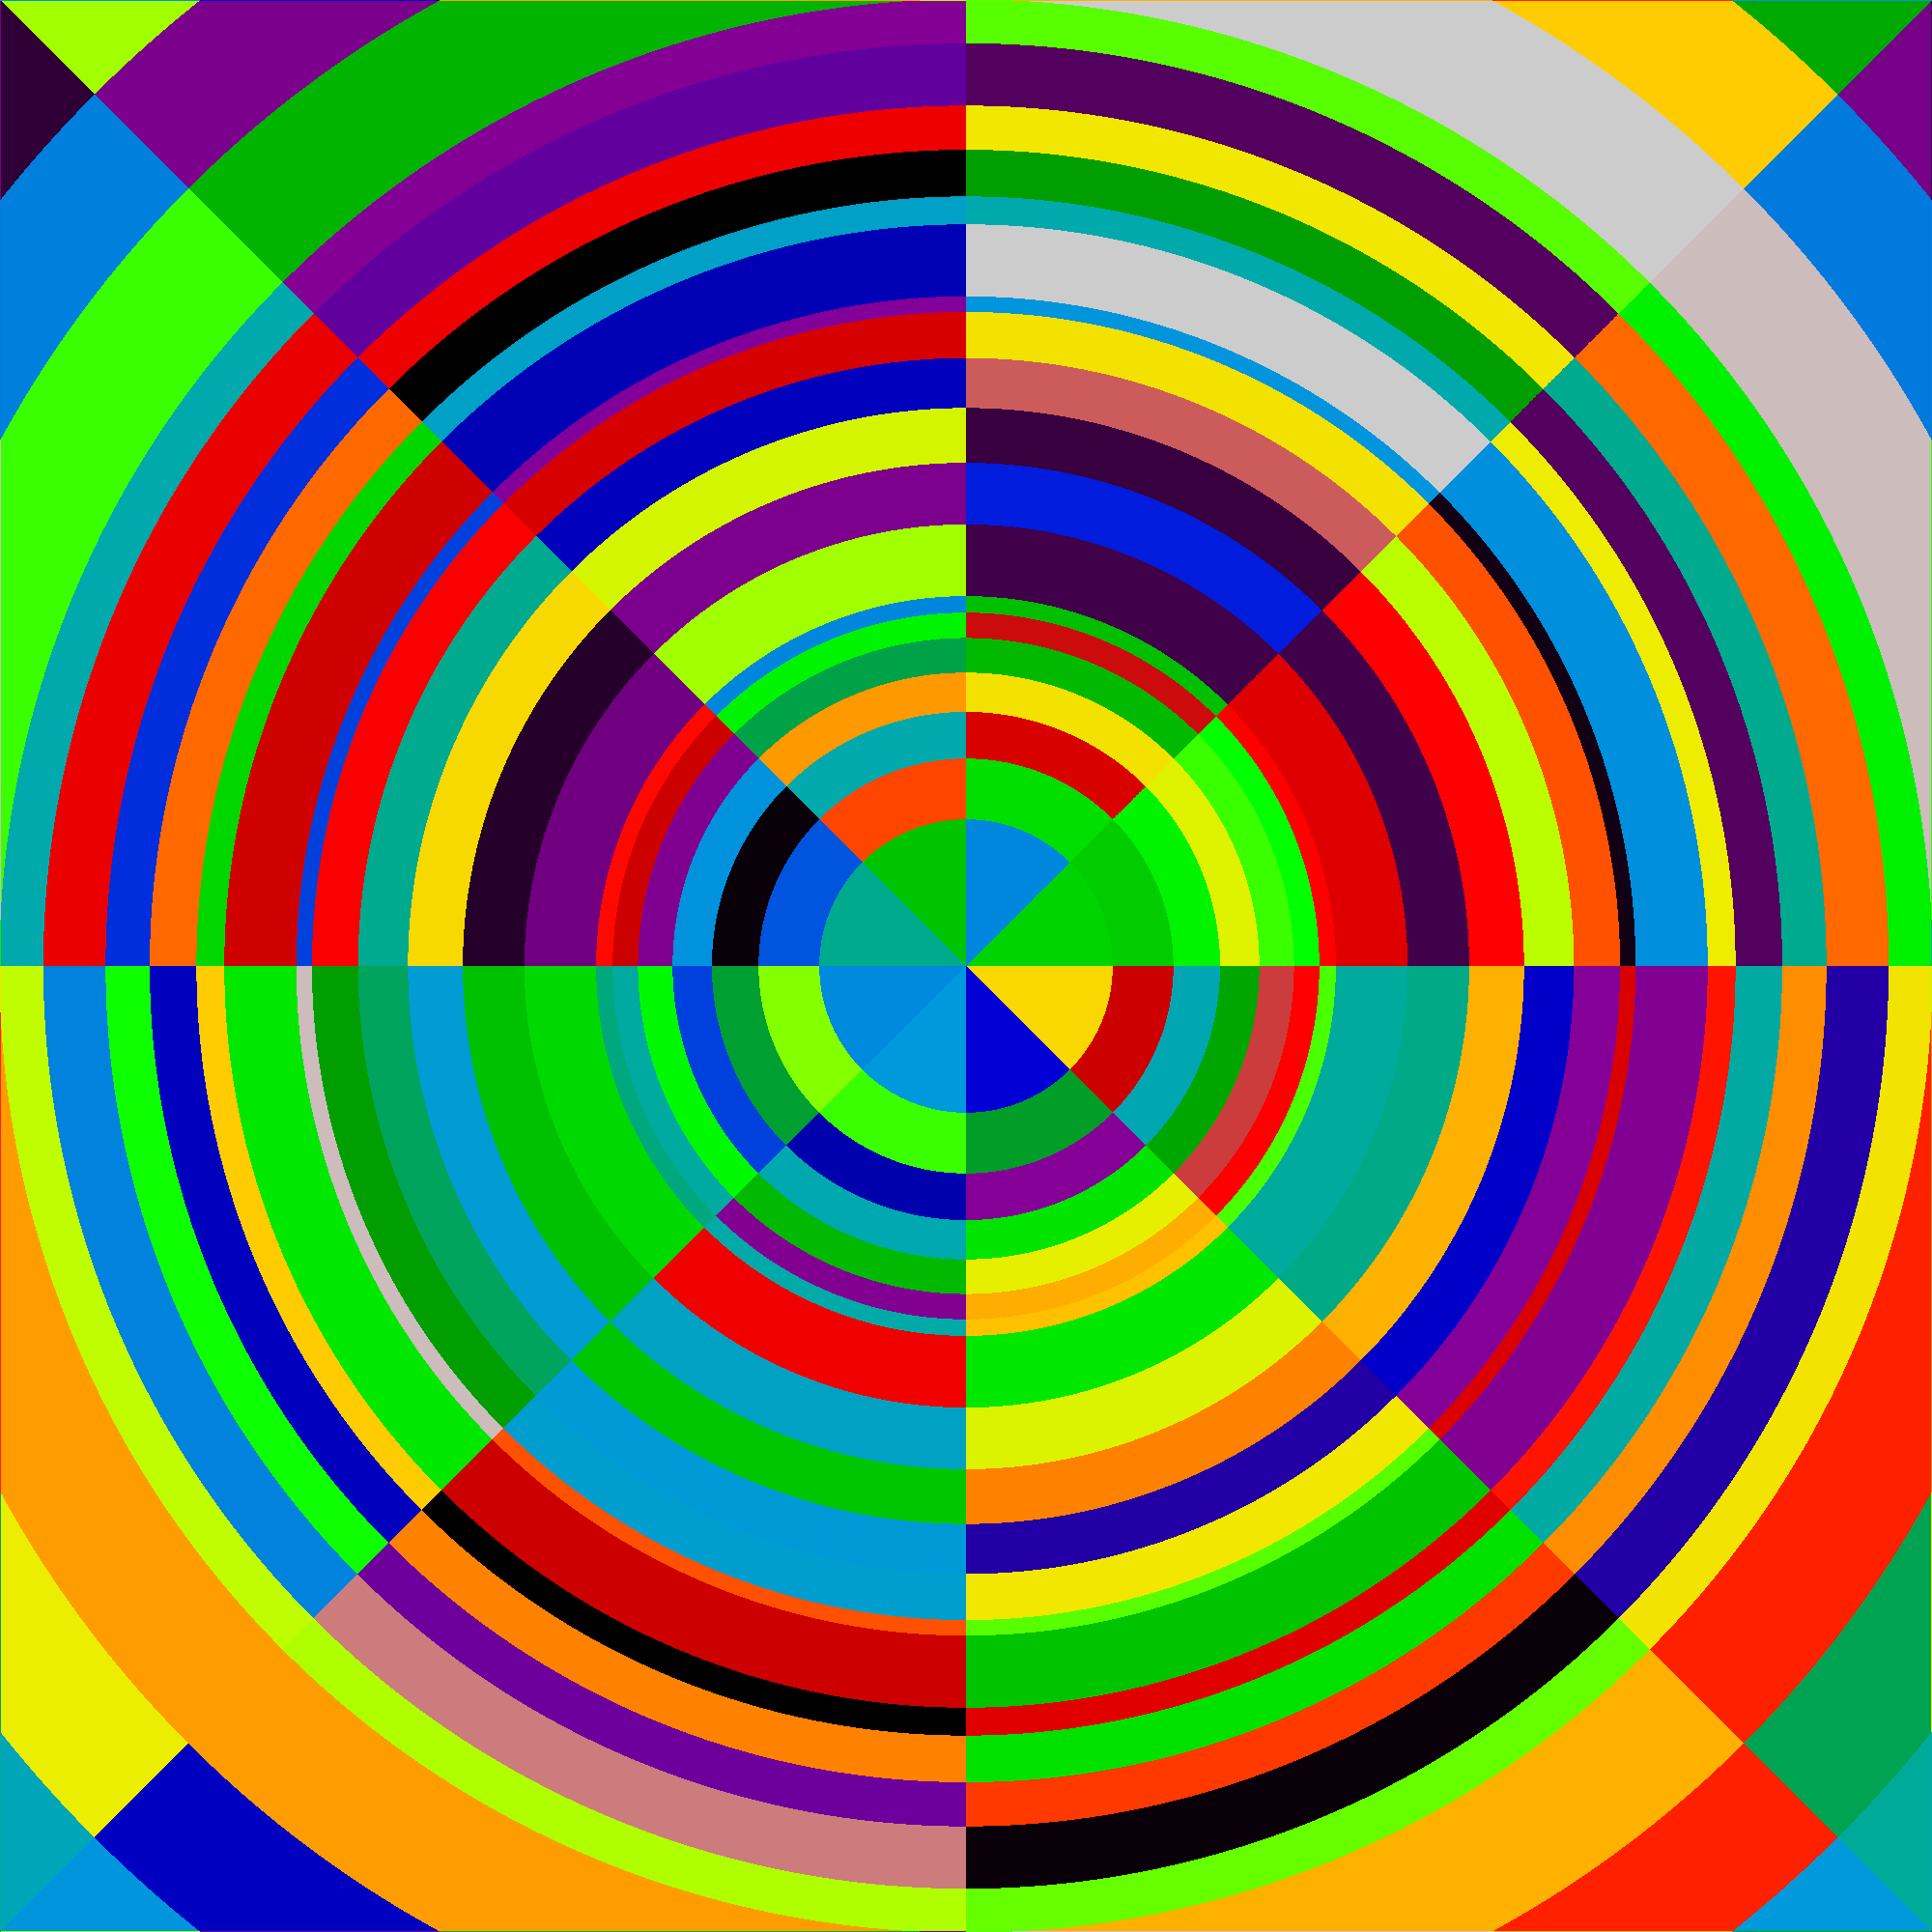
\includegraphics[width=0.8\linewidth]{figures/quantification/fsrs/fsrs-bp}
  \caption{}
  \label{fig:chap8-bp}
\end{subfigure}%
\caption[FSR discretization meshes applied to BEAVRS pin cells]{The \ac{FSR} spatial mesh used for fuel pins (a), control rod guide tubes (b), instrument tubes (c) and burnable poisons (d). Diagrams of each pin type color-coded by material are shown in Fig.~\ref{fig:chap7-pin-cells}.}.
\label{fig:chap8-pin-cell-fsrs}
\end{figure}

\begin{figure}[hb!]
\centering
\begin{subfigure}{0.45\textwidth}
  \centering
  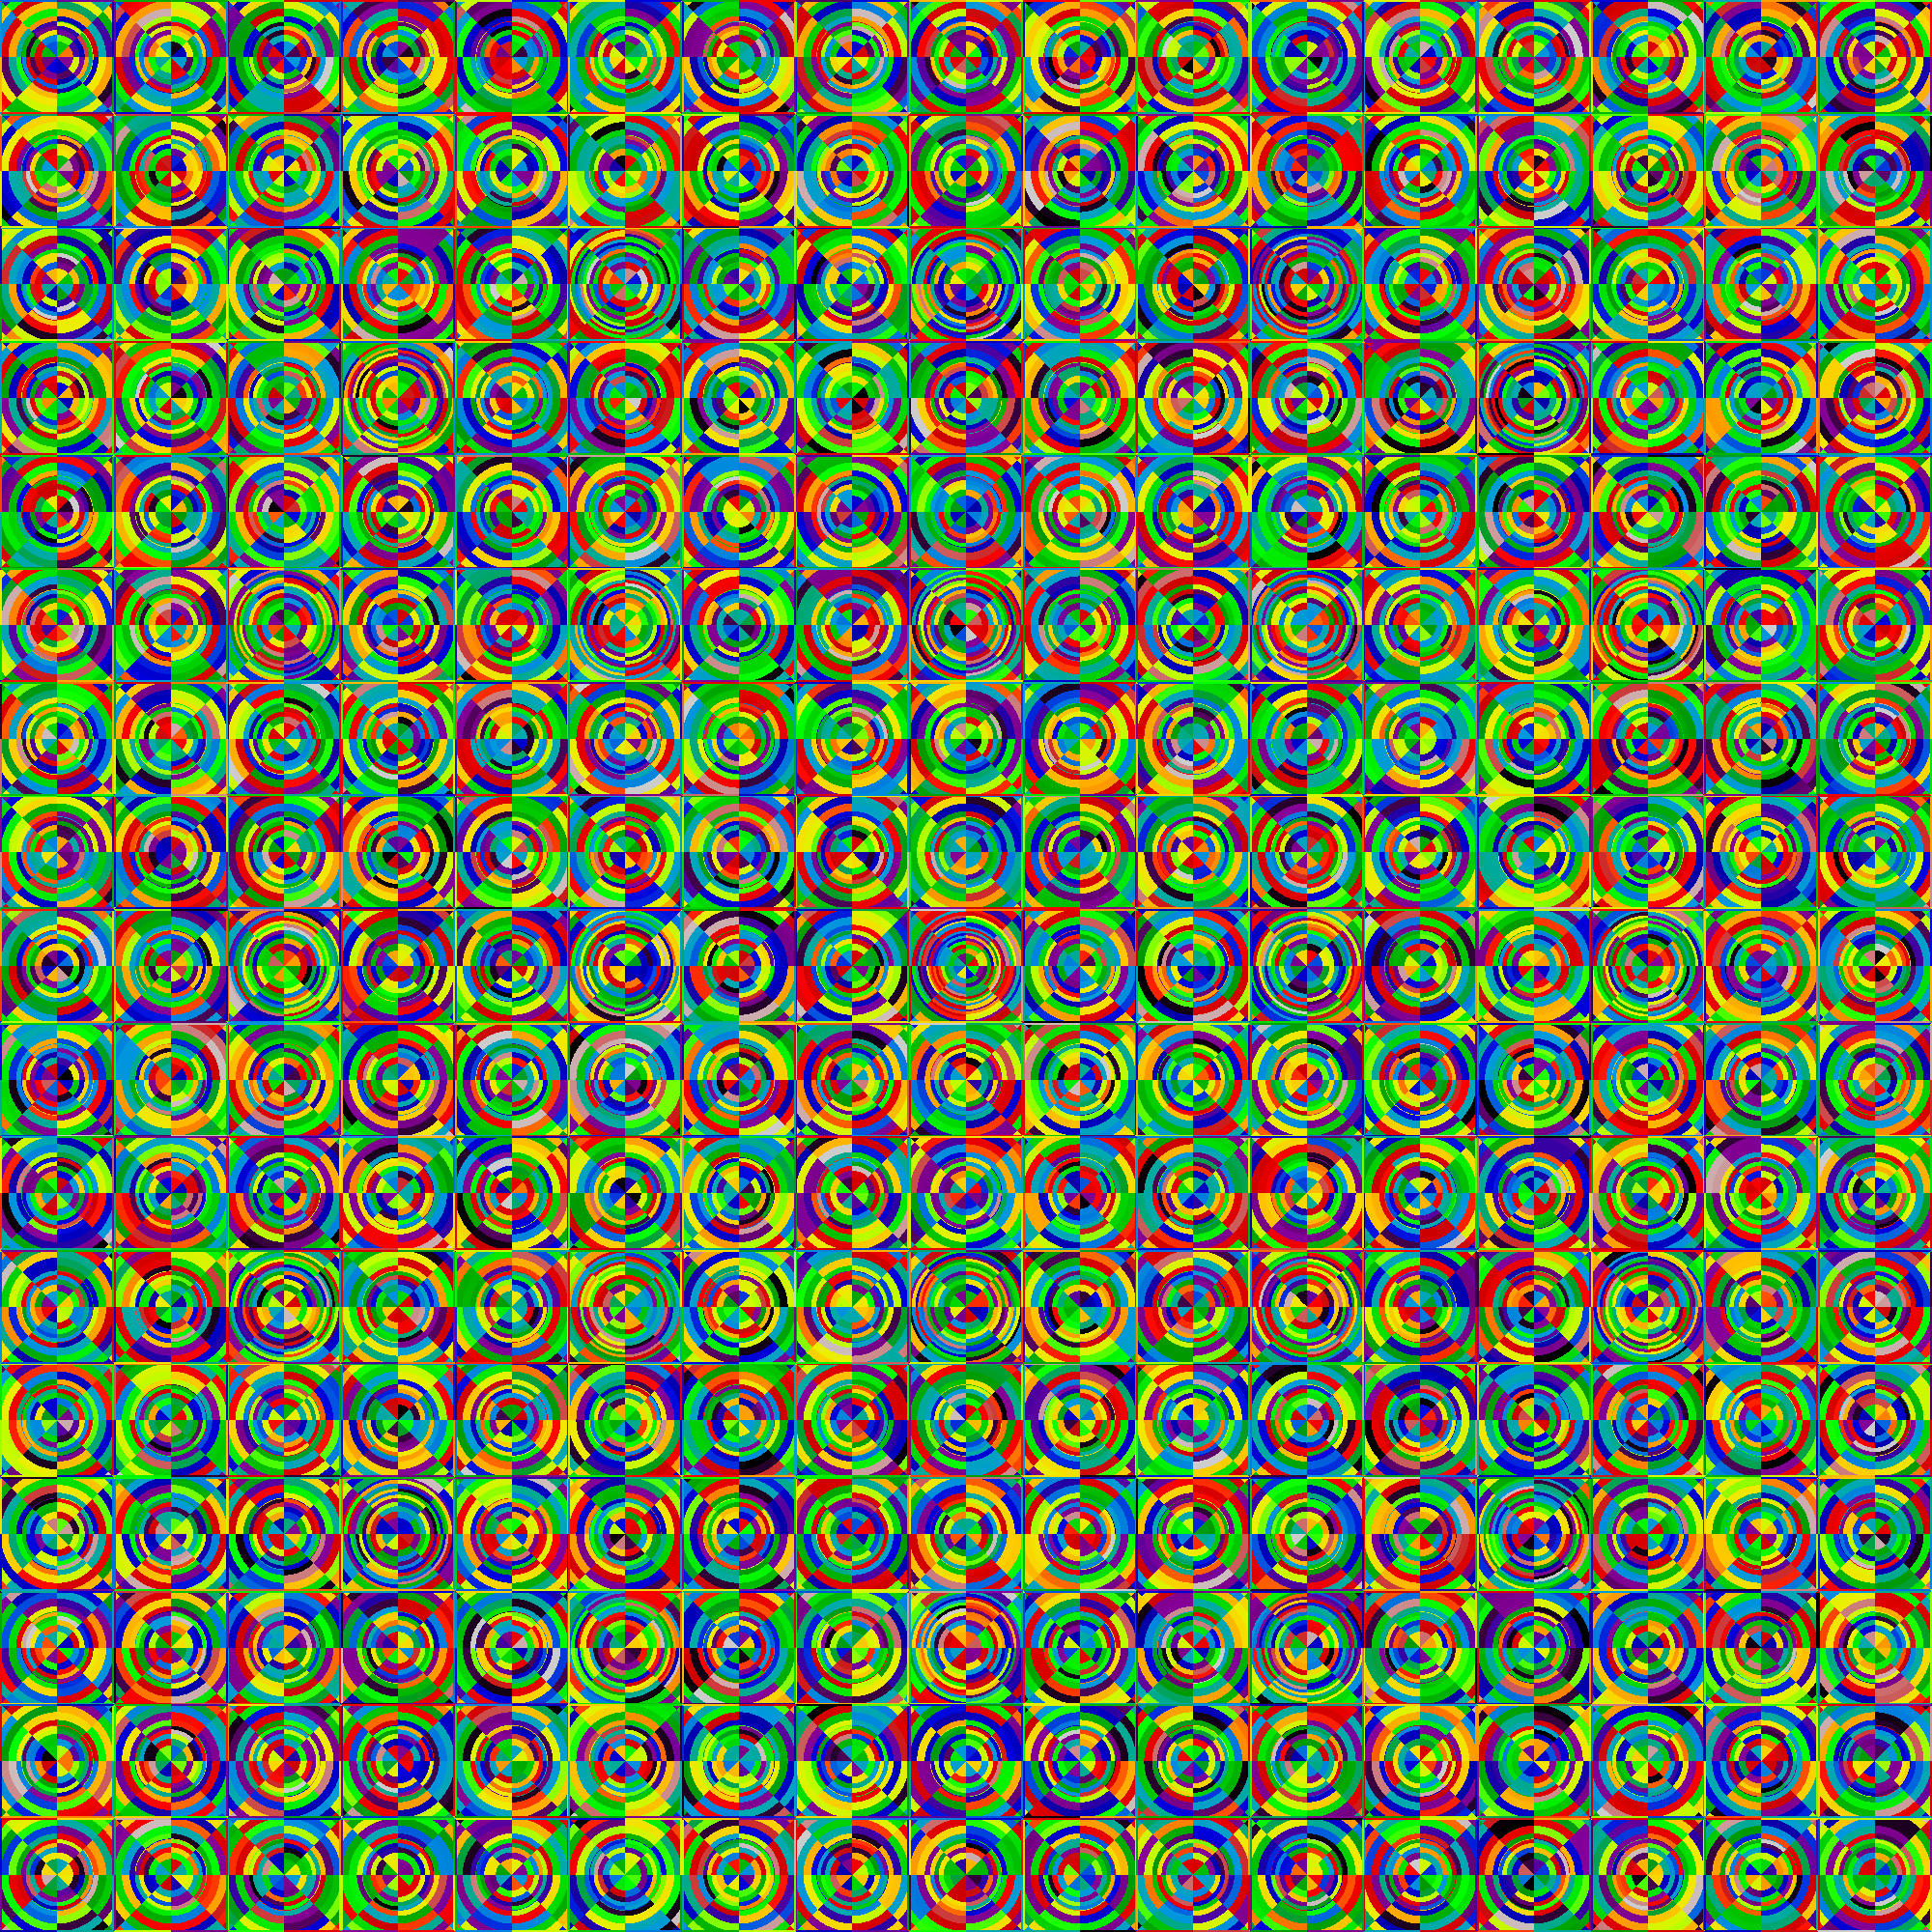
\includegraphics[width=0.87\linewidth]{figures/quantification/fsrs/fsrs-assm-16}
  \caption{}
  \label{fig:chap8-assm-1.6-fsrs}
\end{subfigure}%
\begin{subfigure}{0.45\textwidth}
  \centering
  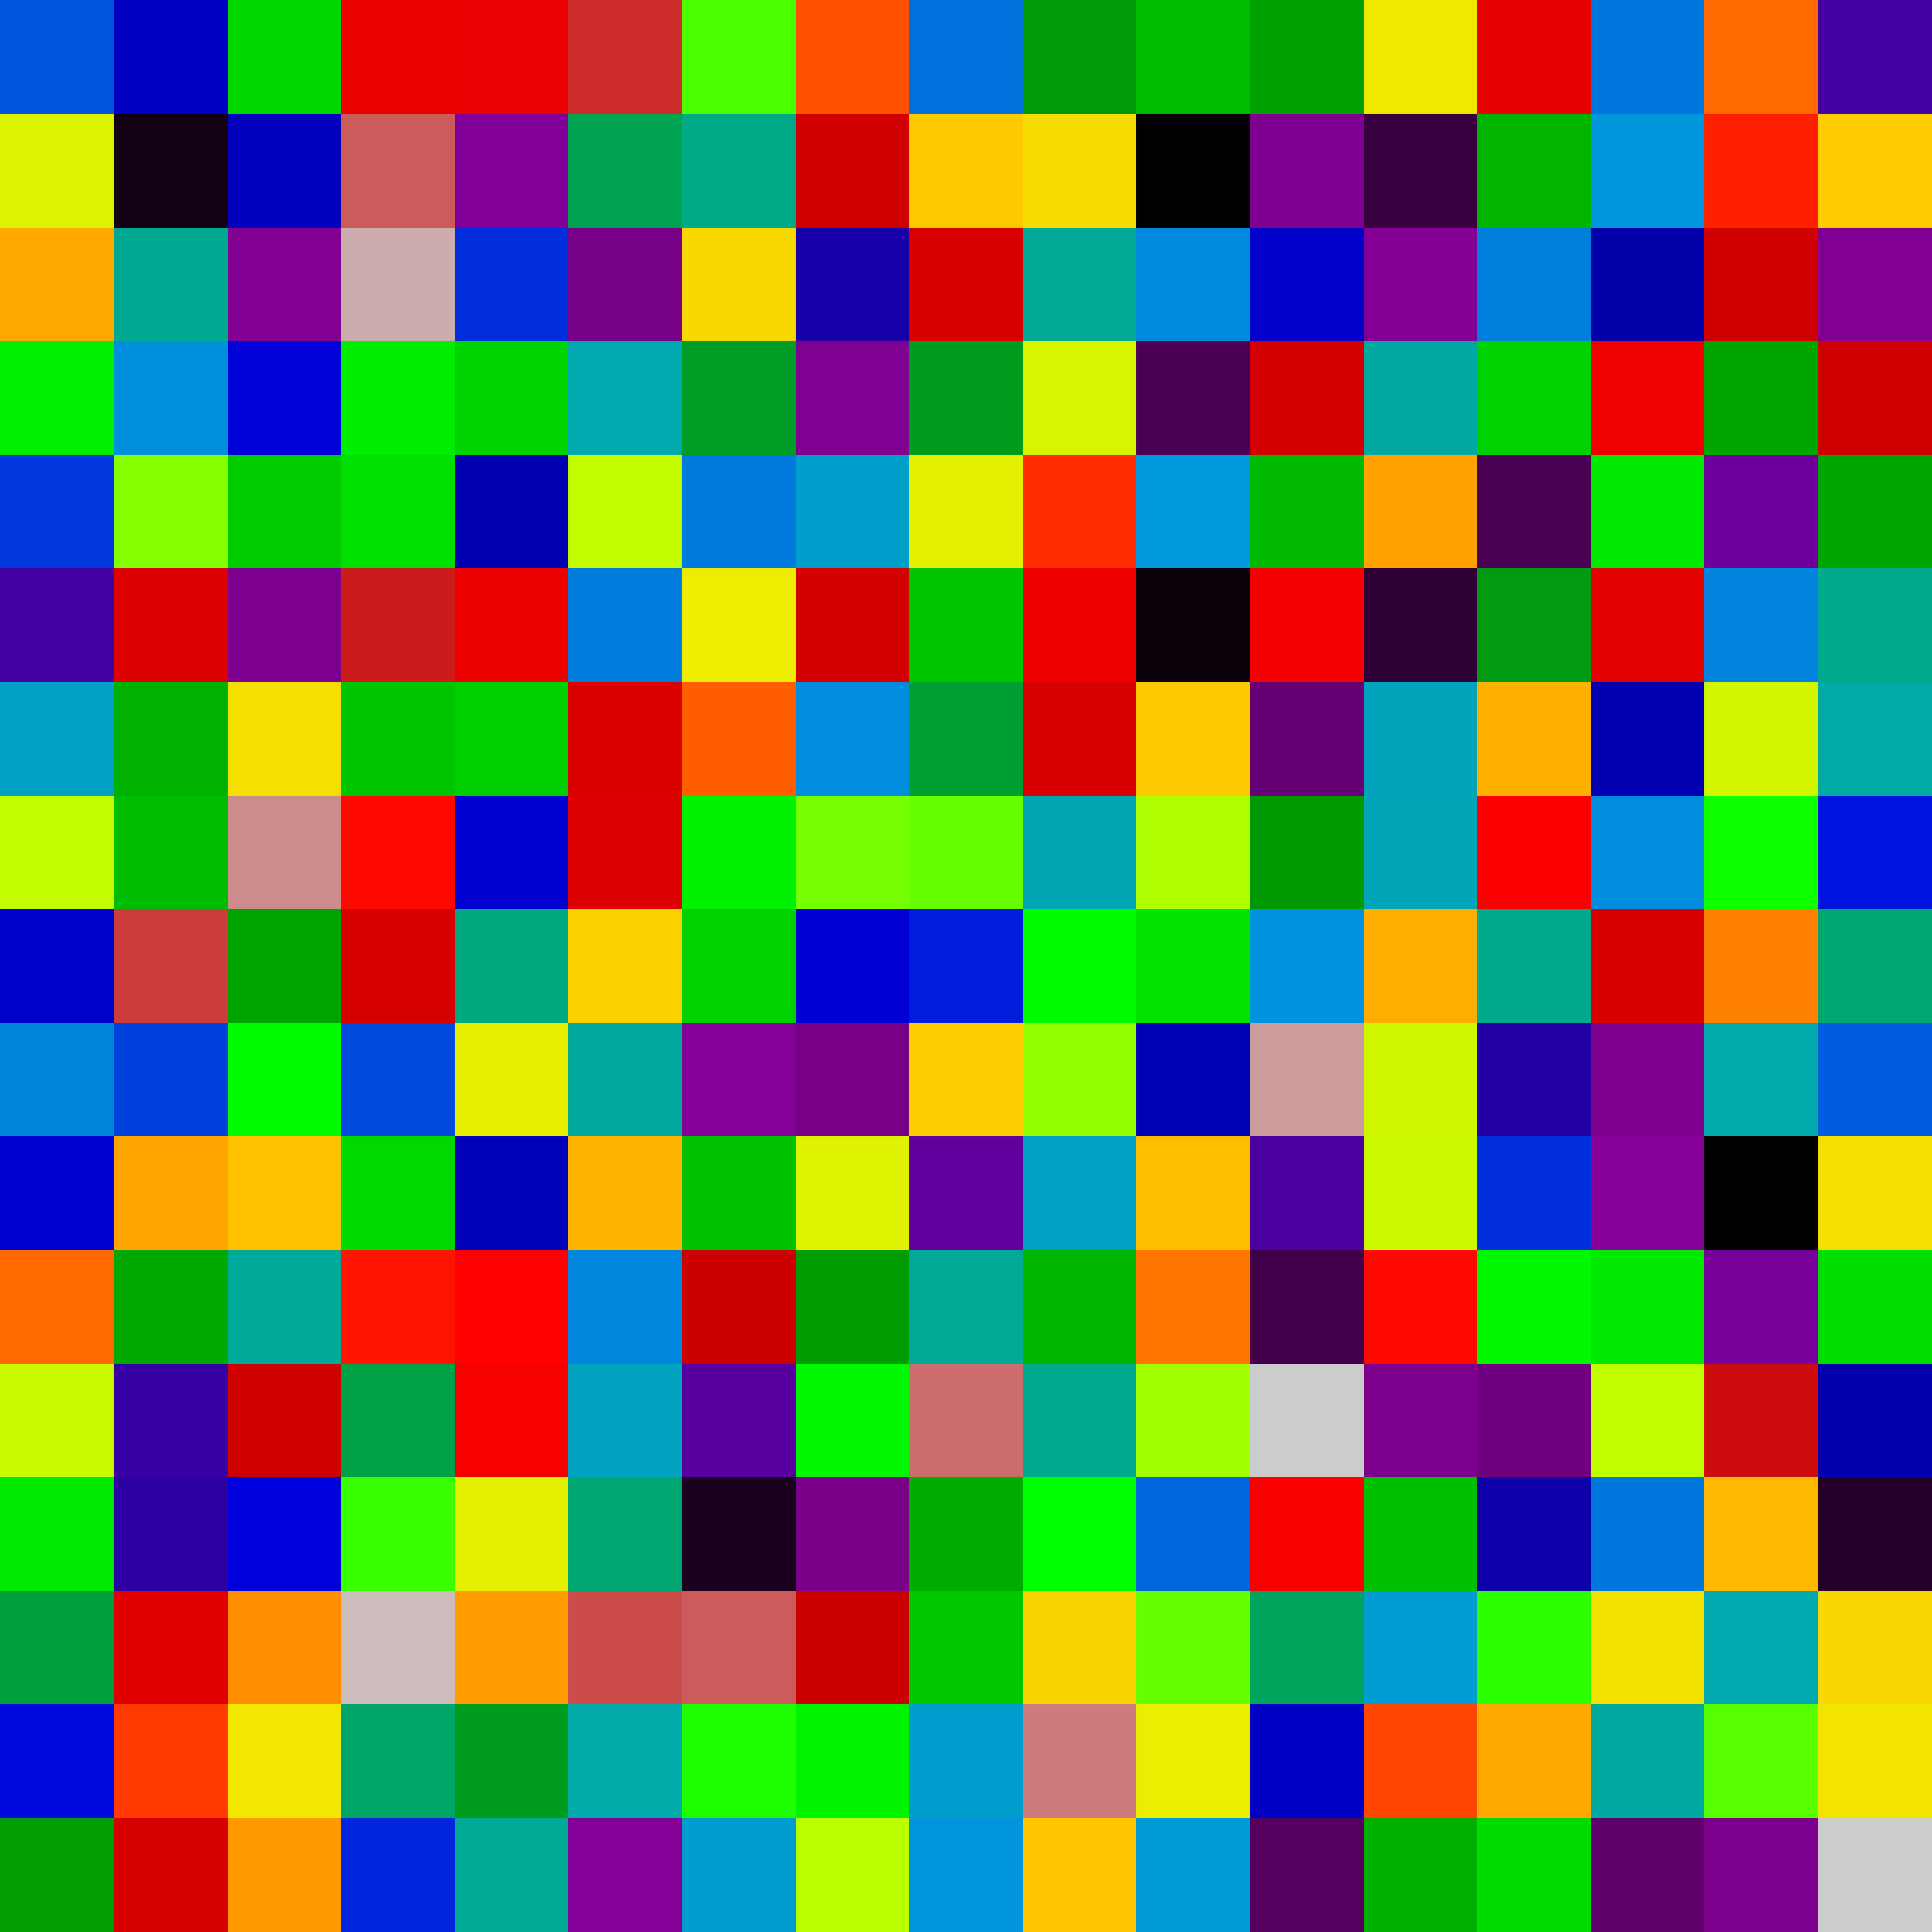
\includegraphics[width=0.87\linewidth]{figures/quantification/cmfd/cmfd-cells-assm}
  \caption{}
  \label{fig:chap8-assm-1.6-cmfd-cells}
\end{subfigure}
\begin{subfigure}{0.45\textwidth}
  \centering
  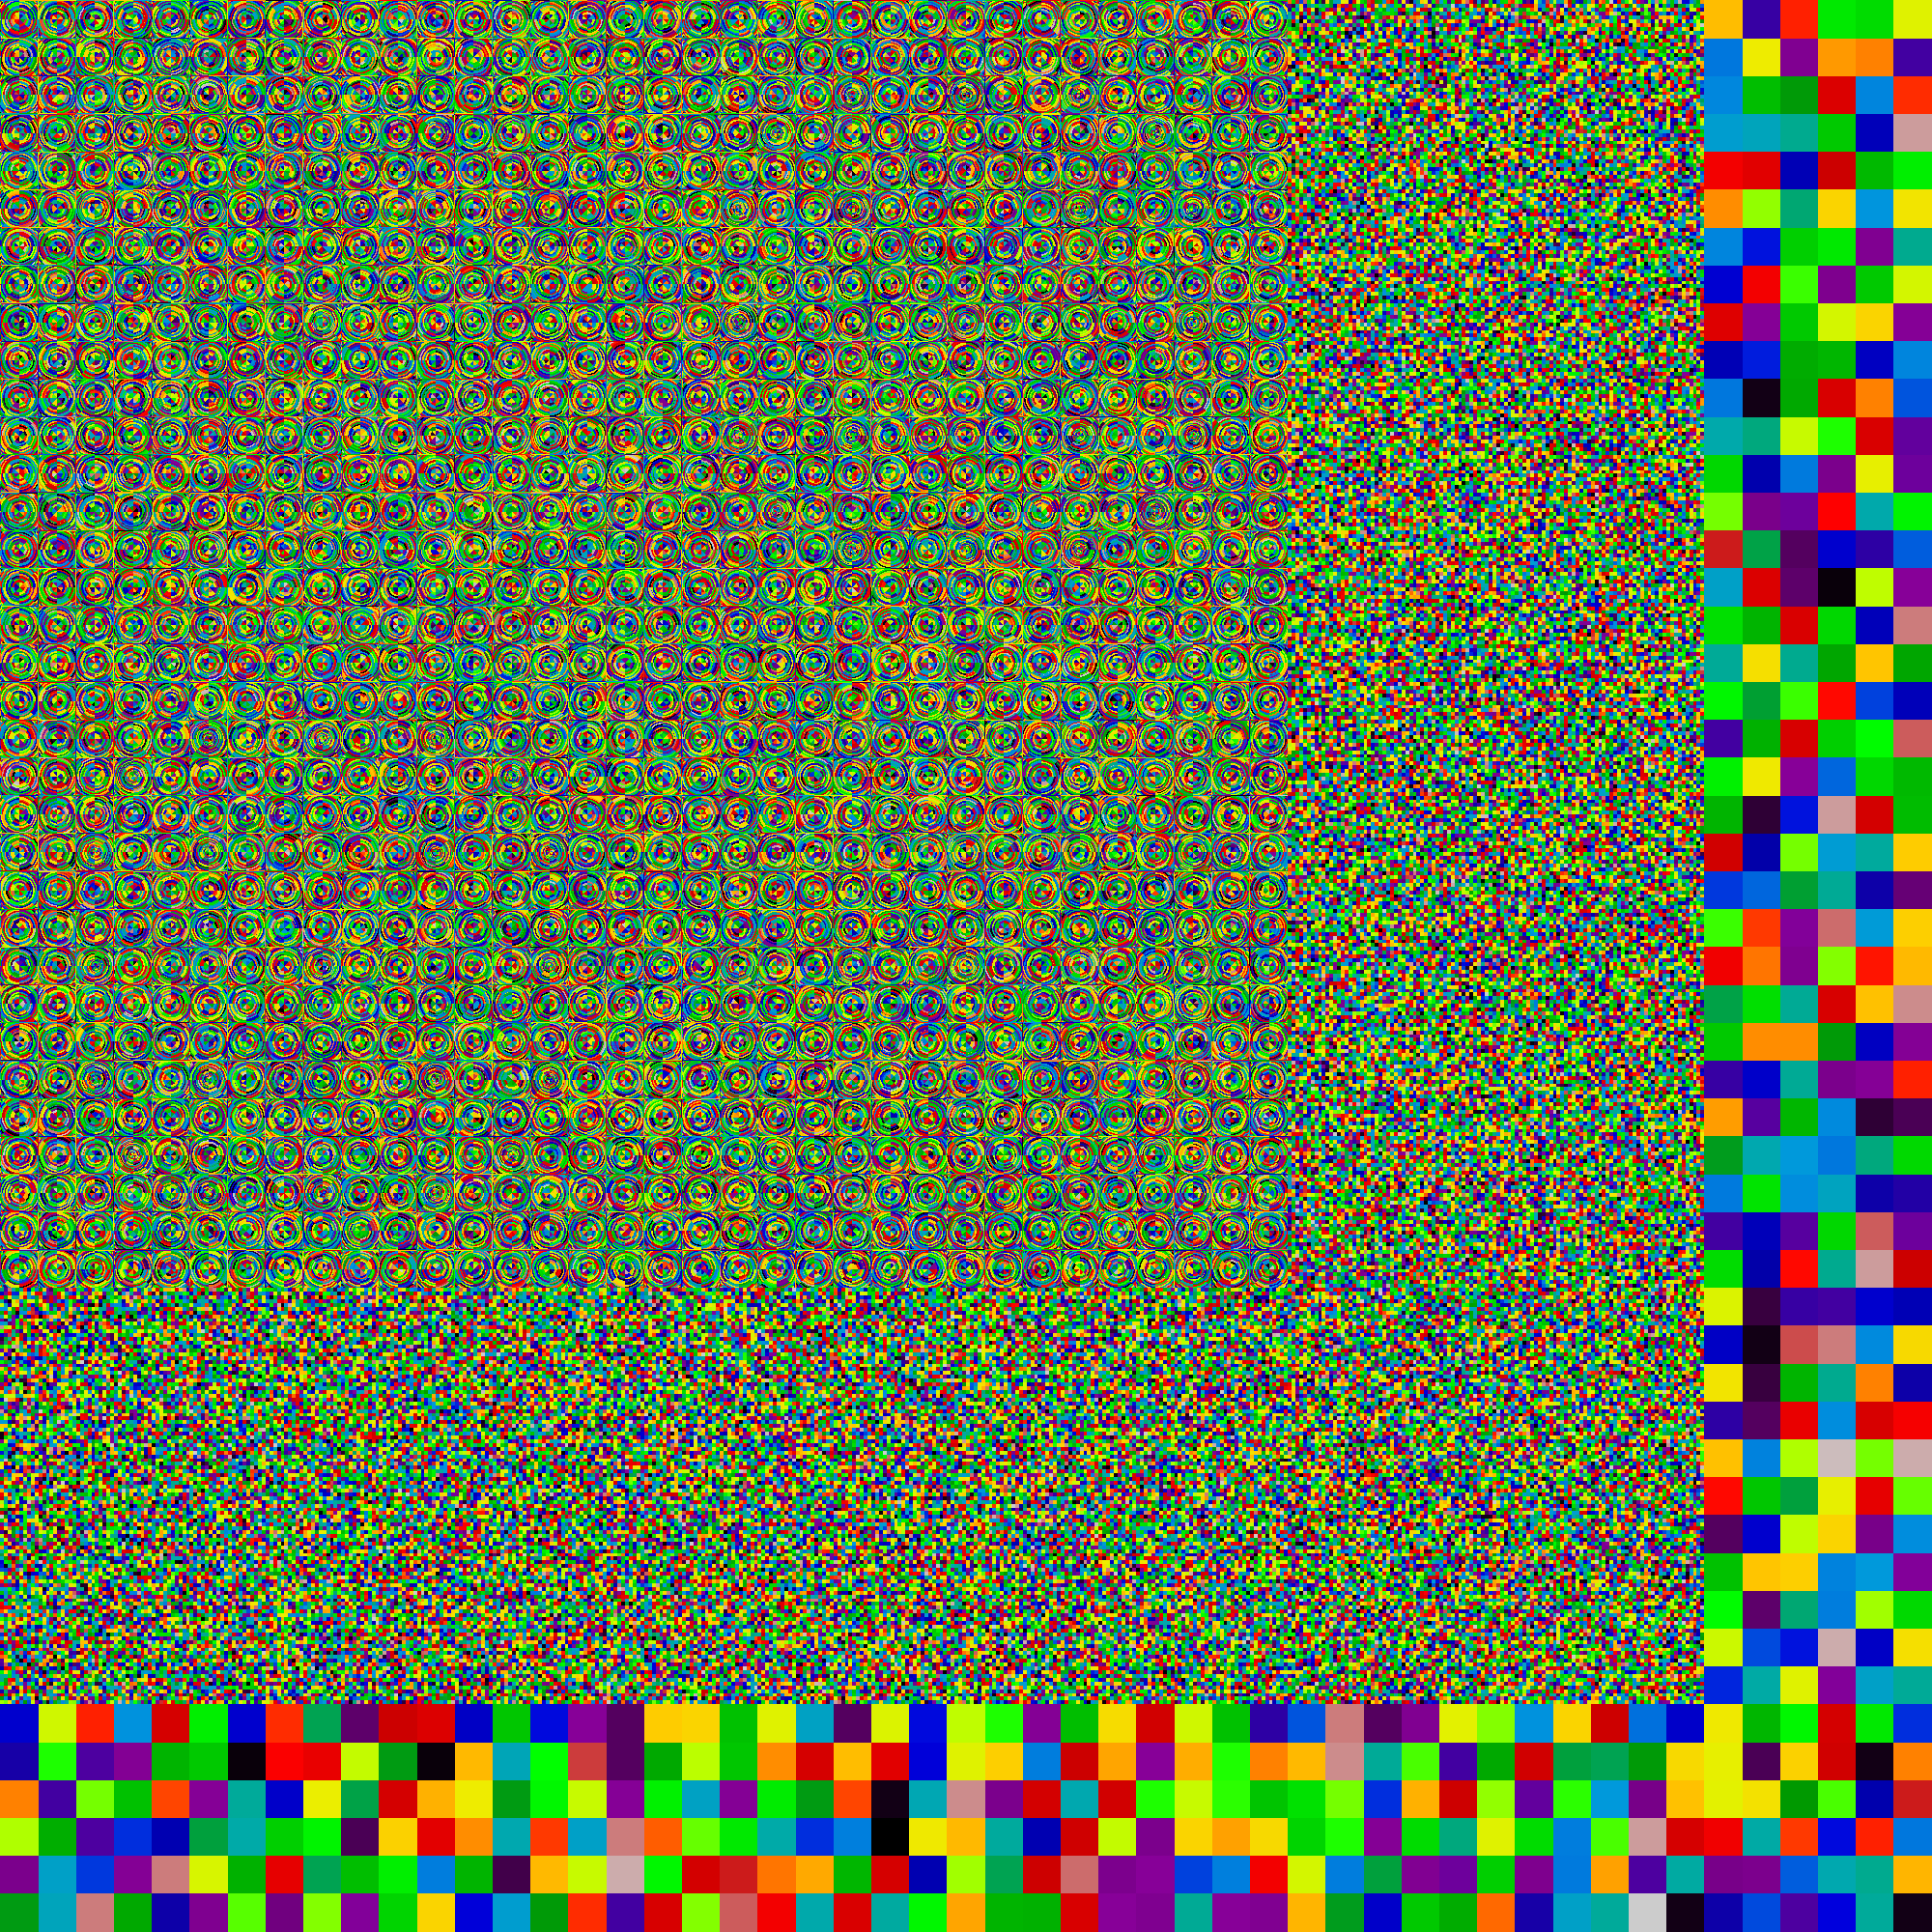
\includegraphics[width=0.87\linewidth]{figures/quantification/fsrs/fsrs-reflector}
  \caption{}
  \label{fig:chap8-reflector-fsrs}
\end{subfigure}%
\begin{subfigure}{0.45\textwidth}
  \centering
  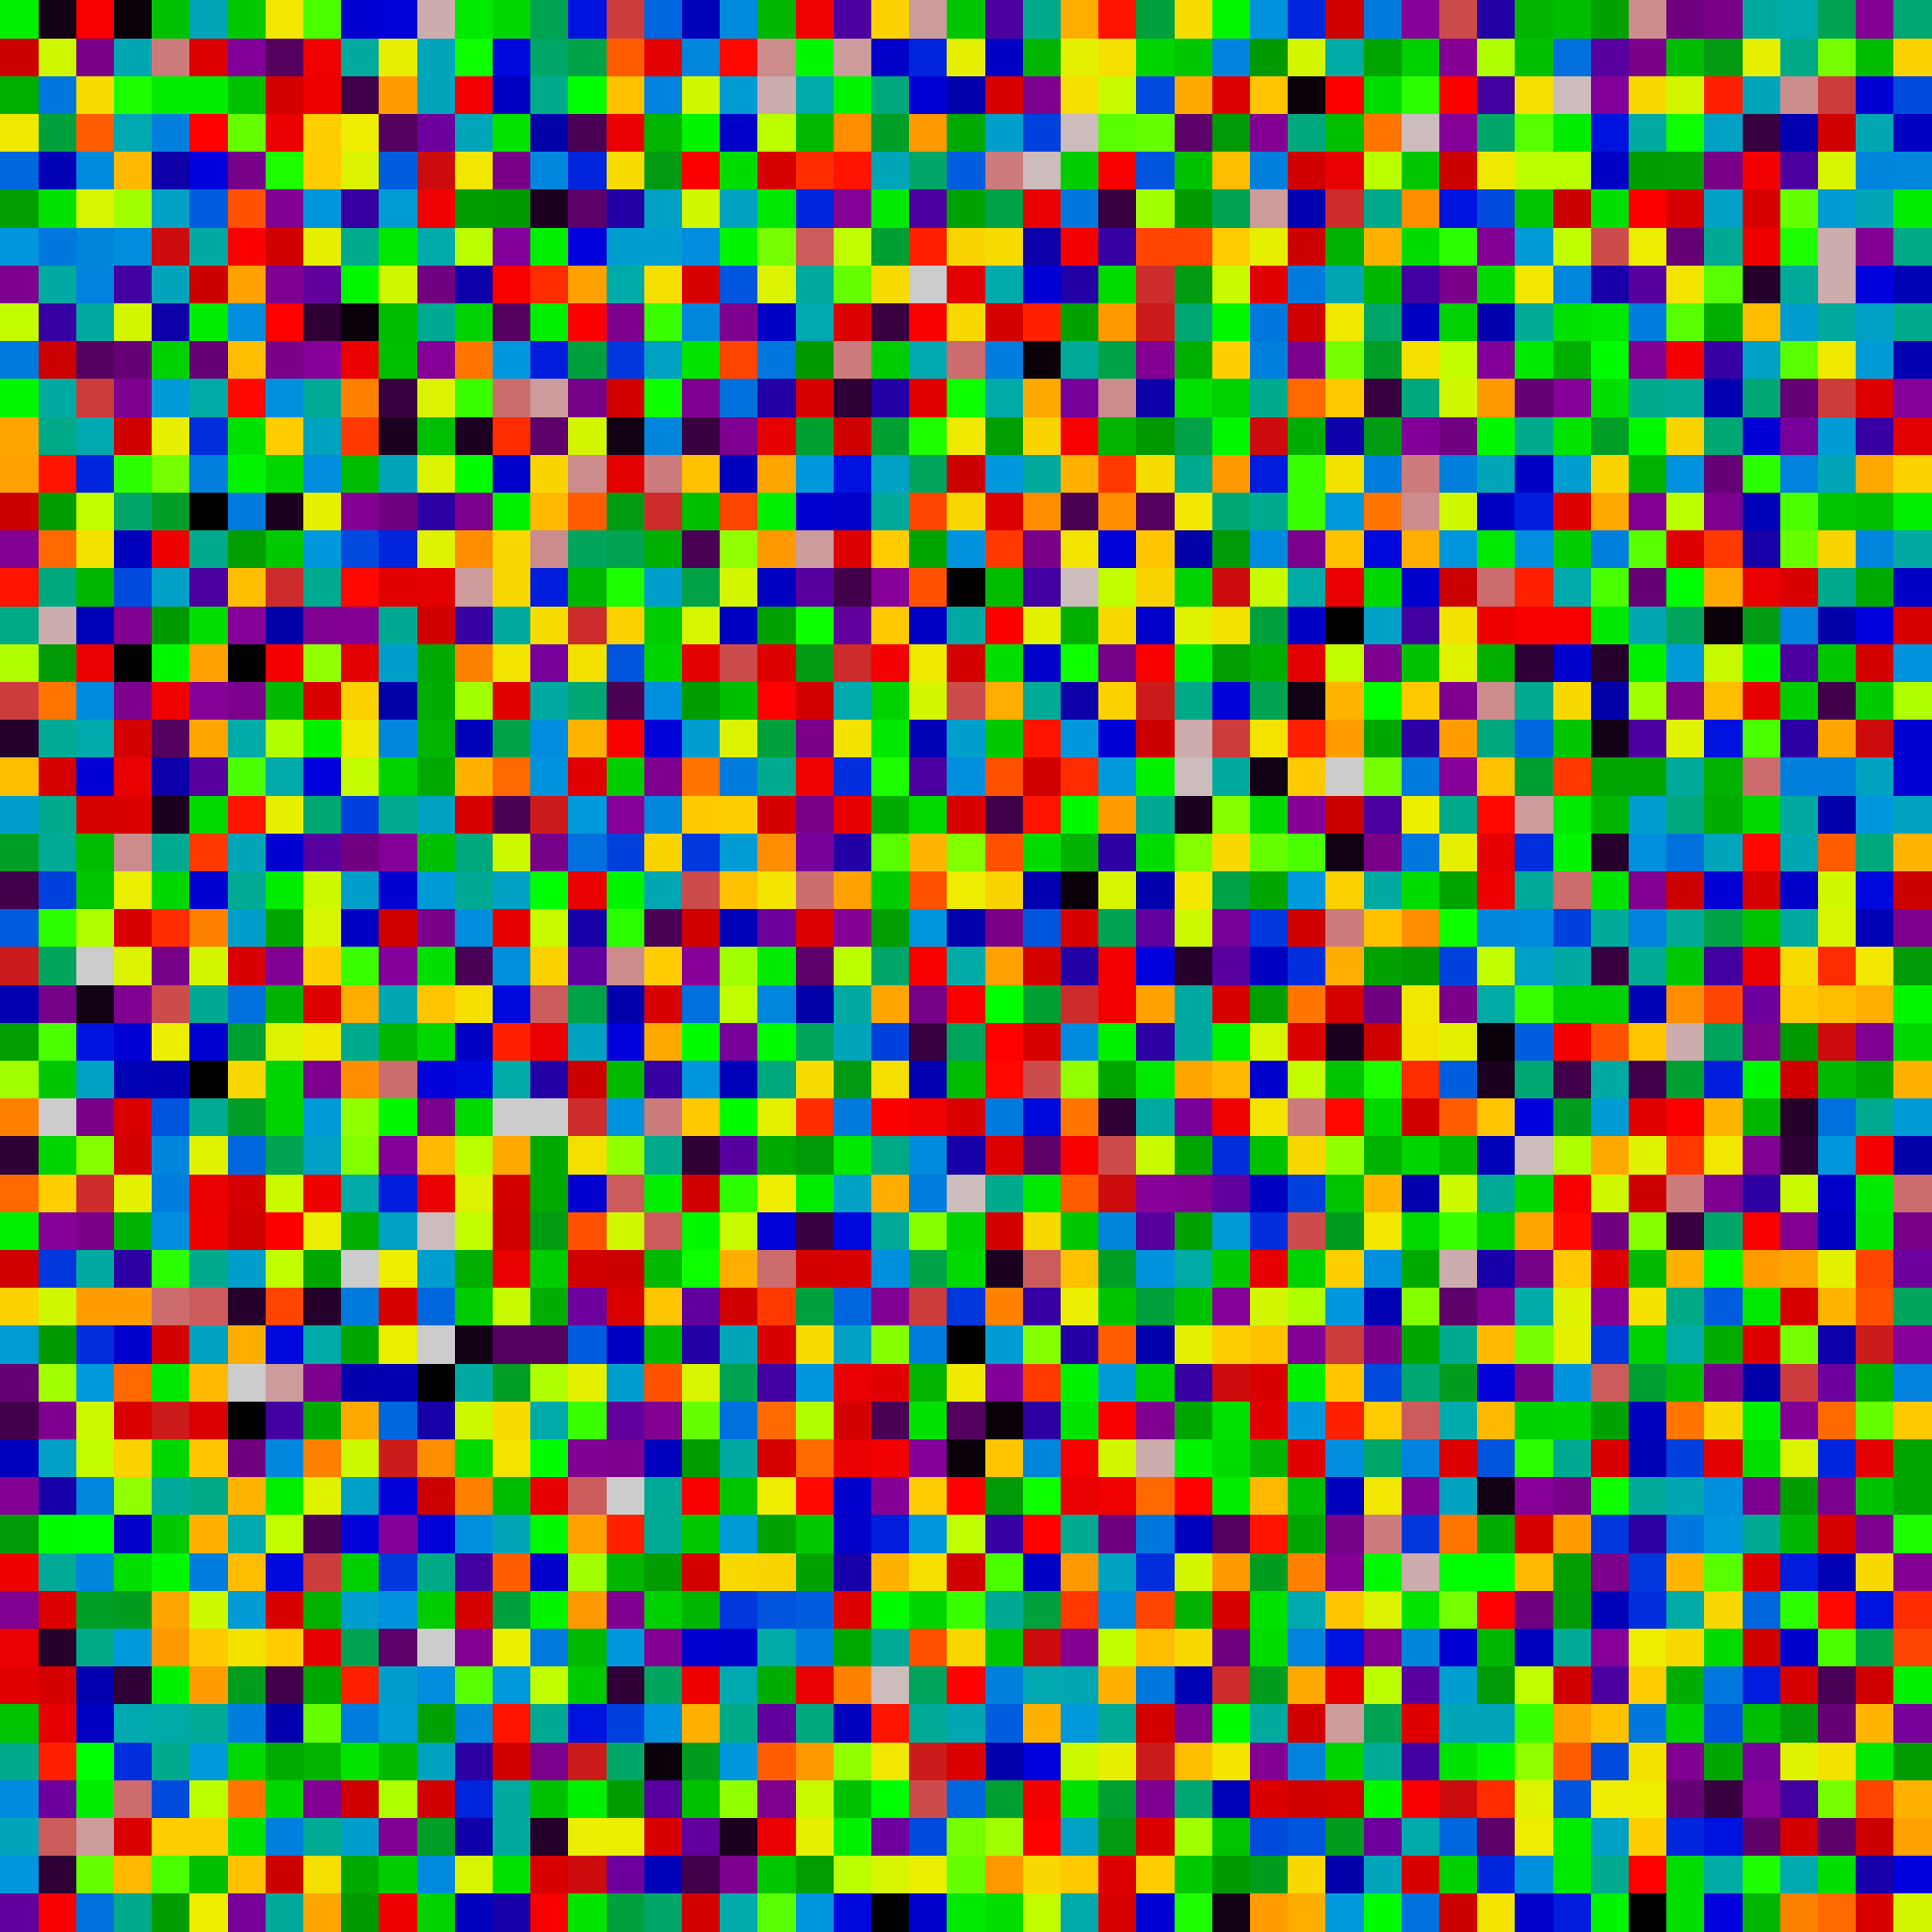
\includegraphics[width=0.87\linewidth]{figures/quantification/cmfd/cmfd-cells-reflector}
  \caption{}
  \label{fig:chap8-reflector-cmfd-cells}
\end{subfigure}
\begin{subfigure}{0.45\textwidth}
  \centering
  
\includegraphics[width=0.87\linewidth]{figures/quantification/fsrs/fsrs-full-core-quarter-pin-cmfd}
  \caption{}
  \label{fig:chap8-full-core-fsrs}
\end{subfigure}%
\begin{subfigure}{0.45\textwidth}
  \centering
  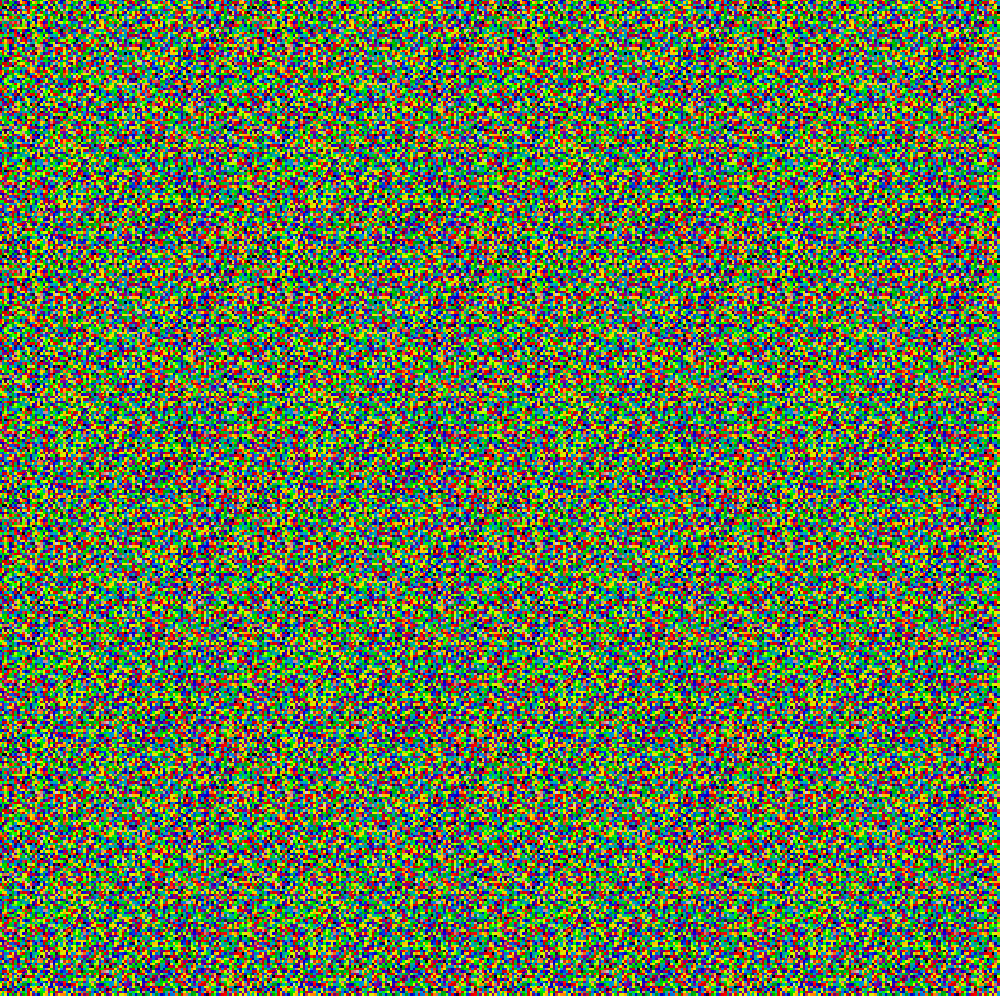
\includegraphics[width=0.87\linewidth]{figures/quantification/cmfd/cmfd-cells-full-core-quarter-pin-cmfd}
  \caption{}
  \label{fig:chap8-full-core-cmfd-cells}
\end{subfigure}
\caption[FSR discretization and CMFD cells for heterogeneous benchmarks]{\ac{FSR} (left) and \ac{CMFD} (right) meshes for a fuel assembly (a) and (b), a 2$\times$2 colorset with reflector (c) and (d), and quarter core \ac{BEAVRS} benchmark (e) and (f).}
\label{fig:chap8-assm-fsrs-cmfd-cells}
\end{figure}

The spatially discretized pin cells were used in each of the six heterogeneous benchmarks. The \ac{FSR} discretizations for an individual fuel assembly, 2$\times$2 colorset with a water reflector, and the upper right quadrant of the \ac{BEAVRS} core are depicted in Fig.~\ref{fig:chap8-assm-fsrs-cmfd-cells}. The water reflector in the 2$\times$2 colorset was discretized using a mesh shown to converge the solution for the similarly designed C5G7 benchmark~\cite{lewis2003c5g7} in~\cite{boyd2014ms}. In particular, the 13.85824 cm (equivalent to 11 pin cells) of water reflector nearest the fuel assemblies was discretized in a 0.125984 cm $\times$ 0.125984 cm rectilinear mesh, equivalent to a 10$\times$10 mesh in each pin. The 7.55904 cm (equivalent to 6 pin cells) of water reflector furthest from the fuel assemblies was discretized in a 1.25984 cm $\times$ 1.25984 cm pin-wise mesh.

Each type of pin cell was discretized in the same way for the quarter core \ac{BEAVRS} model. A 0.31496 cm $\times$ 0.31496 cm mesh (equivalent to a 4$\times$4 mesh in each pin) was applied in the water reflector. The mesh in the reflector was coarser than the mesh used in the reflector for the 2$\times$2 colorset since a finer mesh was not computationally practical for the quarter core \ac{BEAVRS} model, nor needed due to th presence of the steel baffle. A quarter pin-wise \ac{CMFD} mesh (\textit{i.e.}, 0.62992 cm $\times$ 0.62992 cm) was employed for the \ac{BEAVRS} model, which discretized the core barrel and vessel into a corresponding \ac{FSR} mesh.


%%%%%%%%%%%%%%%%%%%%%%%%%%%%%%%%%%%%%%%%%%%%%%%%%%%%%%%%%%%%%%%%%%%%%%%%%%%%%%%
\section{Analysis of Multi-Group Results}
\label{sec:chap8-mg-results}

Each of the six benchmarks was modeled with OpenMOC using \ac{MGXS} generated by the infinite, null and degenerate spatial homogenization schemes. The eigenvalues and pin-wise fission and U-238 capture rates computed by OpenMOC are compared to the reference OpenMC solutions in Secs.~\ref{subsec:chap8-eigenvalues},~\ref{subsec:chap8-fiss-rates} and~\ref{subsec:chap8-capt-rates}, respectively.

%%%%%%%%%%%%%%%%%%%%%%%%
\subsection{Eigenvalues}
\label{subsec:chap8-eigenvalues}

The OpenMOC eigenvalues were compared to the reference OpenMC eigenvalues from Tab.~\ref{table:chap7-ref-eigenvalues}. The eigenvalue bias $\Delta\rho$ was computed from Eqn.~\ref{eqn:chap5-delta-rho} in units of \ac{pcm}. The bias is listed for each benchmark, energy group structure and spatial homogenization scheme in Tab.~\ref{table:chap8-openmoc-eigenvalues}. It should be recalled that isotropic in lab scattering is used by OpenMC to compute both the reference solution and the \ac{MGXS}. If anisotropic scattering were employed in OpenMC, one would expect quite different biases without a robust implementation of a higher order scattering kernel in OpenMOC.

As expected, the eigenvalue bias is highly dependent on energy group structure. In general, a positive bias is exhibited for 2 groups with an increasingly negative trend with more groups. The bias is remarkably consistent between -100 and -250 \ac{pcm} for 70 groups for all of the benchmarks. This slightly negative bias is reminiscent of the -200 \ac{pcm} bias observed for the 1D slab and 2D pin cell \ac{PWR} benchmarks when modeled with 70 groups in Chap.~\ref{chap:biases}. The introduction of a reflector region in the 2$\times$2 colorset increases the bias to over 1700 \ac{pcm} for all homogenization schemes for 2 groups, but the bias is greatly reduced when modeled with more groups.

%\vspace{0.1in} 

\renewcommand{\arraystretch}{0.9}% Tighter

\begin{table}[ht!]
  \centering
  \caption[OpenMOC eigenvalue bias for heterogeneous benchmarks]{OpenMOC eigenvalue bias $\Delta\rho$ for heterogeneous benchmarks with varying spatial homogenization schemes and energy group structures.}
  \small
  \label{table:chap8-openmoc-eigenvalues}
  \vspace{6pt}
  \begin{tabular}{l l R{2.5cm} R{2.5cm} R{2.5cm}}
  \toprule
  \rowcolor{lightgray}
  & & \multicolumn{3}{S[table-format=6.1]}{\cellcolor{lightgray} {$\bm{\Delta\rho}$ \textbf{[pcm]}}} \\
  \multirow{-2}{*}{\cellcolor{lightgray} \bf Benchmark} &
  \multirow{-2}{*}{\cellcolor{lightgray} \bf \ac{MGXS} Scheme} &
  \multicolumn{1}{r}{{\cellcolor{lightgray} \bf 2-Group}} &
  \multicolumn{1}{r}{{\cellcolor{lightgray} \bf 8-Group}} &
  \multicolumn{1}{r}{{\cellcolor{lightgray} \bf 70-Group}} \\
  \midrule
\multirow{3}{*}{\parbox{2.5cm}{1.6\% Assm}} & Infinite & -132 & -68 & 31 \\
& Null & 60 & -72 & -161 \\
& Degenerate & 62 & -72 & -161 \\
  \midrule
\multirow{3}{*}{\parbox{2.5cm}{3.1\% Assm}} & Infinite & -188 & -98 & 29 \\
& Null & 95 & -79 & -202 \\
& Degenerate & 98 & -80 & -202 \\
  \midrule
\multirow{3}{*}{\parbox{2.5cm}{3.1\% Assm w/ 20 BPs}} & Infinite & 392 & 20 & -76 \\
& Null & -136 & -163 & -252 \\
& Degenerate & -160 & -161 & -248 \\
  \midrule
\multirow{3}{*}{\parbox{2.5cm}{2$\times$2 Colorset}} & Infinite & 267 & -149 & -16 \\
& Null & 27 & -93 & -196 \\
& Degenerate & 11 & -93 & -193 \\
  \midrule
\multirow{3}{*}{\parbox{2.5cm}{2$\times$2 Colorset w/ Reflector}} & Infinite & 2103 & 267 & 46 \\
& Null & 1818 & 478 & -142 \\
& Degenerate & 1765 & 487 & -132 \\
  \midrule
\multirow{3}{*}{\parbox{2.5cm}{BEAVRS Full Core}} & Infinite & 2000 & 296 & 103 \\
& Null & 2181 & 406 & -128 \\
& Degenerate & 2179 & 408 & -125 \\
  \bottomrule
\end{tabular}
\end{table}

%\footnotetext{The \ac{BEAVRS} benchmark is modeled with 40 groups; all other benchmarks are modeled with 70 groups.\label{note1}}

The eigenvalue bias is also dependent on the spatial homogenization scheme used to compute \ac{MGXS} in the fuel. It should first be noted that the eigenvalues are consistent for the null and degenerate schemes to within 10 \ac{pcm} with 8 or more groups for all benchmarks. This is expected since the \ac{MGXS} for each scheme is homogenized from the same flux and should preserve globally-integrated reaction rates. In contrast, the infinite scheme's eigenvalues differ by up to 300 \ac{pcm} from the null/degenerate schemes, with no marked trend across benchmarks and energy group structures.

%The infinite scheme also agrees with the null and degenerate schemes to within 50 \ac{pcm} for all of the benchmarks with 8 and 70 groups. However, the infinite scheme produces a markedly larger bias for the 2-group structure. The introduction of \acp{BP} to the 3.1\% enriched fuel assembly substantially increases the bias to over 1000 \ac{pcm} for the infinite scheme, while only increasing the magnitude by roughly 50 \ac{pcm} for the null and degenerate schemes. This disparity in the eigenvalue bias between the infinite and null/degenerate schemes is further increased with the introduction of a reflector to the 2$\times$2 colorset, and other heterogeneities in the quarter core \ac{BEAVRS} model.

% PUT THIS IN ANALYSIS SECTION???
%These results demonstrate the importance of using a relatively fine energy group structure -- in this case, 40 and 70 groups -- to accurately predict the eigenvalue in deterministic multi-group calculations. In addition, use of the spatially self-shielded flux from the heterogeneous geometry to collapse 2-group cross sections in the null and degenerate schemes enabled significantly more accurate eigenvalues than was possible with the infinite lattice flux. 

\begin{emphbox}
\textbf{A consistent eigenvalue bias between OpenMC and OpenMOC of less than 250 \ac{pcm} is observed for all benchmarks and homogenization schemes with 70 groups. The eigenvalues for the null and degenerate schemes are consistent to within 10 \ac{pcm} for eight or more groups due to reaction rate preservation.}
\end{emphbox}

%%%%%%%%%%%%%%%%%%%%%%%%%%%%%%%%%%%%%%%
\subsection{Fission Rate Distributions}
\label{subsec:chap8-fiss-rates}

The OpenMOC energy-integrated pin-wise fission rates were compared to the reference OpenMC fission rates from Figs.~\Crefrange{fig:chap7-fiss-rates-1.6-assm}{fig:chap7-fiss-rates-full-core}. The percent relative errors for each pin's fission rates were computed and the maximum and mean errors are listed for each benchmark, energy group structure and spatial homogenization scheme in Tabs.~\ref{table:chap8-openmoc-max-fiss-rates} and~\ref{table:chap8-openmoc-mean-fiss-rates}, respectively. In particular, the maximum errors are the maximum of the absolute values of the errors along with the appropriate sign, while the mean errors are the averages of the absolute error magnitudes.

As was the case for the eigenvalues, the fission rate errors are highly dependent on energy group structure. As expected, the maximum and mean errors are substantially reduced with finer energy group structures for all benchmarks and spatial homogenization schemes. The maximum fission rates are 2 -- 11\% in 2 groups for the individual fuel assembly and 2$\times$2 colorset benchmarks, respectively, but decrease to less than 1\% when modeled with 70 groups. The mean fission rate errors likewise decrease with finer energy group structures, and are less than 0.2\% in magnitude for the assembly and colorset benchmarks for all homogenization schemes with 70 groups.

The fission rate errors are somewhat dependent on the spatial homogenization scheme used to compute \ac{MGXS} in the fuel. In particular, the degenerate scheme produces slightly smaller maximum and mean errors than the null and infinite schemes. The error reduction is largest in 2 groups, and is less significant for more groups. The null and infinite schemes do not exhibit a systematic difference in their fission rate errors.

%\vspace{0.1in}

\begin{table}[ht!]
  \centering
  \caption[Maximum OpenMOC fission rate errors]{OpenMOC maximum fission rate percent relative errors for heterogeneous benchmarks with varying spatial homogenization schemes and energy group structures.}
  \small
  \label{table:chap8-openmoc-max-fiss-rates}
  \vspace{6pt}
  \begin{tabular}{l l R{2.5cm} R{2.5cm} R{2.5cm}}
  \toprule
  \rowcolor{lightgray}
  & & \multicolumn{3}{c}{\cellcolor{lightgray} \textbf{Max Error [\%]}} \\
  \multirow{-2}{*}{\cellcolor{lightgray} \bf Benchmark} &
  \multirow{-2}{*}{\cellcolor{lightgray} \bf \ac{MGXS} Scheme} &
  \multicolumn{1}{r}{{\cellcolor{lightgray} \bf 2-Group}} &
  \multicolumn{1}{r}{{\cellcolor{lightgray} \bf 8-Group}} &
  \multicolumn{1}{r}{{\cellcolor{lightgray} \bf 70-Group}} \\
  \midrule
\multirow{3}{*}{\parbox{2.5cm}{1.6\% Assm}} & Infinite & 2.387 & 0.643 & 0.375 \\
& Null & 2.379 & 0.638 & 0.380 \\
& Degenerate & 1.903 & 0.726 & 0.315 \\
  \midrule
\multirow{3}{*}{\parbox{2.5cm}{3.1\% Assm}} & Infinite & 2.779 & 0.729 & 0.433 \\
& Null & 2.748 & 0.719 & 0.437 \\
& Degenerate & 2.151 & 0.832 & 0.372 \\
  \midrule
\multirow{3}{*}{\parbox{2.5cm}{3.1\% Assm w/ 20 BPs}} & Infinite & -3.090 & -0.707 & 0.372 \\
& Null & -3.139 & -0.701 & 0.380 \\
& Degenerate & 1.915 & -0.689 & 0.331 \\
  \midrule
\multirow{3}{*}{\parbox{2.5cm}{2$\times$2 Colorset}} & Infinite & -5.964 & -1.425 & 0.418 \\
& Null & -6.059 & -1.428 & 0.463 \\
& Degenerate & -5.339 & -1.442 & 0.427 \\
  \midrule
\multirow{3}{*}{\parbox{2.5cm}{2$\times$2 Colorset w/ Reflector}} & Infinite & 11.024 & 2.773 & 0.670 \\
& Null & -16.330 & -2.855 & 0.764 \\
& Degenerate & -11.158 & -2.821 & 0.602 \\
  \midrule
\multirow{3}{*}{\parbox{2.5cm}{BEAVRS Quarter Core}} & Infinite & -79.994 & -31.934 & 2.103 \\
& Null & -85.893 & -32.357 & 1.829 \\
& Degenerate & -85.596 & -32.382 & 1.728 \\
  \bottomrule
\end{tabular}
\end{table}

\begin{table}[ht!]
  \centering
  \caption[Mean OpenMOC fission rate errors]{OpenMOC mean absolute fission rate percent relative errors for heterogeneous benchmarks with varying spatial homogenization schemes and energy group structures.}
  \small
  \label{table:chap8-openmoc-mean-fiss-rates}
  \vspace{6pt}
  \begin{tabular}{l l R{2.5cm} R{2.5cm} R{2.5cm}}
  \toprule
  \rowcolor{lightgray}
  & & \multicolumn{3}{c}{\cellcolor{lightgray} \textbf{Mean Error [\%]}} \\
  \multirow{-2}{*}{\cellcolor{lightgray} \bf Benchmark} &
  \multirow{-2}{*}{\cellcolor{lightgray} \bf \ac{MGXS} Scheme} &
  \multicolumn{1}{r}{{\cellcolor{lightgray} \bf 2-Group}} &
  \multicolumn{1}{r}{{\cellcolor{lightgray} \bf 8-Group}} &
  \multicolumn{1}{r}{{\cellcolor{lightgray} \bf 70-Group}} \\
  \midrule
\multirow{3}{*}{\parbox{2.5cm}{1.6\% Assm}} & Infinite & 0.951 & 0.231 & 0.073 \\
& Null & 0.943 & 0.229 & 0.074 \\
& Degenerate & 0.687 & 0.240 & 0.079 \\
  \midrule
\multirow{3}{*}{\parbox{2.5cm}{3.1\% Assm}} & Infinite & 1.177 & 0.285 & 0.080 \\
& Null & 1.155 & 0.279 & 0.081 \\
& Degenerate & 0.808 & 0.290 & 0.087 \\
  \midrule
\multirow{3}{*}{\parbox{2.5cm}{3.1\% Assm w/ 20 BPs}} & Infinite & 0.927 & 0.194 & 0.095 \\
& Null & 0.937 & 0.193 & 0.098 \\
& Degenerate & 0.692 & 0.213 & 0.086 \\
  \midrule
\multirow{3}{*}{\parbox{2.5cm}{2$\times$2 Colorset}} & Infinite & 3.152 & 0.690 & 0.108 \\
& Null & 3.132 & 0.690 & 0.120 \\
& Degenerate & 2.918 & 0.702 & 0.120 \\
  \midrule
\multirow{3}{*}{\parbox{2.5cm}{2$\times$2 Colorset w/ Reflector}} & Infinite & 4.964 & 1.029 & 0.147 \\
& Null & 5.471 & 1.080 & 0.178 \\
& Degenerate & 4.731 & 1.065 & 0.138 \\
  \midrule
\multirow{3}{*}{\parbox{2.5cm}{BEAVRS Quarter Core}} & Infinite & 34.831 & 10.391 & 0.492 \\
& Null & 39.355 & 10.541 & 0.323 \\
& Degenerate & 39.520 & 10.474 & 0.336 \\
  \bottomrule
\end{tabular}
\end{table}

The spatial distributions of fission rate errors are plotted as heatmaps for each benchmark in Figs.~\Crefrange{fig:chap8-assm-1.6-fiss-err}{fig:chap8-full-core-fiss-err}. These figures illustrate the fission rate errors for 8 and 70 energy group structures for the null and degenerate schemes; the reaction rate errors for 2, 8, and 70 groups for all three homogenization schemes are compared in Figs.~\Crefrange{fig:quantify-assm-1.6-fiss-err}{fig:quantify-full-core-fiss-err} in App.~\ref{sec:quantify-fiss-rates}. The heatmaps illustrate systematic trends in the pin-wise fission errors which correlate with spatial heterogeneities in each benchmark. In particular, the fission rates are generally underpredicted for pins near \acp{CRGT}, but overpredicted for pins near \acp{BP} and in pins removed from \acp{CRGT}, such as those in the corners of each fuel assembly. The effects due to heterogeneities are further enhanced when differentiating pins which are facially adjacent to \acp{CRGT}, facially and corner adjacent to two \acp{CRGT}, etc. In addition, the error magnitudes are large for pins along the inter-assembly and assembly-reflector interfaces for the 2$\times$2 colorset benchmarks. For the \ac{PWR} benchmarks modeled here, the differential moderation provided by neighboring \acp{CRGT} and reflectors softens the flux for nearby fuel pins and should be modeled when collapsing pin-wise \ac{MGXS} for high-fidelity multi-group transport calculations.

%As noted previously, the energy group structure has a large impact on the error distributions as can be seen from the figures. In addition, the heatmaps illustrate how the degenerate spatial homogenization scheme effectively ``smooths'' the pin-wise errors as compared to the infinite and null schemes. This effect is most pronounced when the benchmarks are modeled with 2-group \ac{MGXS} as shown in App.~\ref{sec:quantify-fiss-rates}. The differential of the errors for pins near \acp{CRGT}, \acp{BP}, and assembly and reflector interfaces is substantially reduced when degenerate homogenization is applied. The difference in the error spatial distributions for the infinite and null schemes is hardly noticeable except for pins near the assembly and reflector interfaces for the 2$\times$2 colorset benchmarks.

\begin{emphbox}
\textbf{The use of degenerate spatial homogenization ``smooths'' the spatial distribution of pin-wise fission rate errors for 2-group \ac{MGXS}. However, the fission rates computed with \ac{MGXS} generated from the infinite, null and degenerate homogenization schemes are very similar with fine 70 group structures.}
\end{emphbox}

\begin{figure}[h!]
\centering
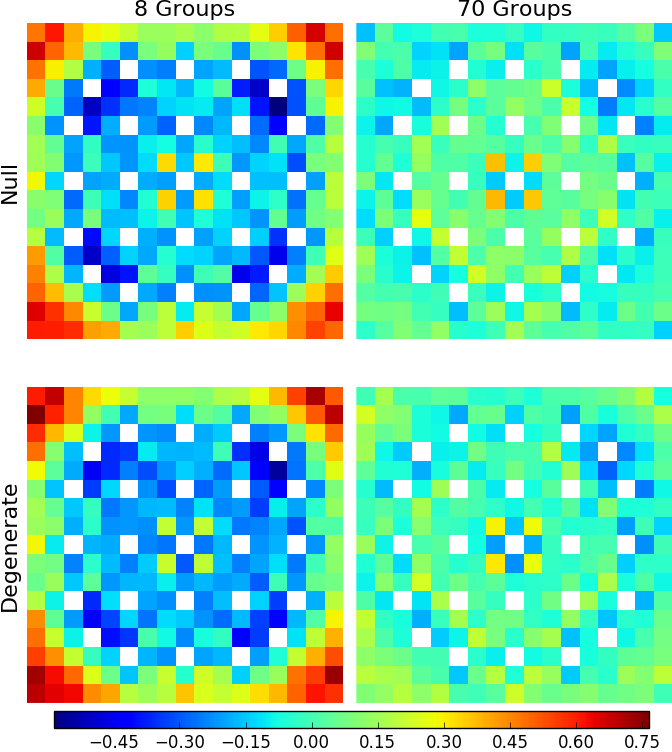
\includegraphics[width=\linewidth]{figures/quantification/assm-16/fiss-err}
\vspace{2mm}
\caption[Fission rate errors for a 1.6\% enriched assembly]{Fission rate percent relative errors for a 1.6\% enriched assembly corresponding to the reference in Fig.~\ref{fig:chap7-fiss-rates-1.6-assm}.}
\label{fig:chap8-assm-1.6-fiss-err}
\end{figure}

\clearpage

\begin{figure}[h!]
\centering
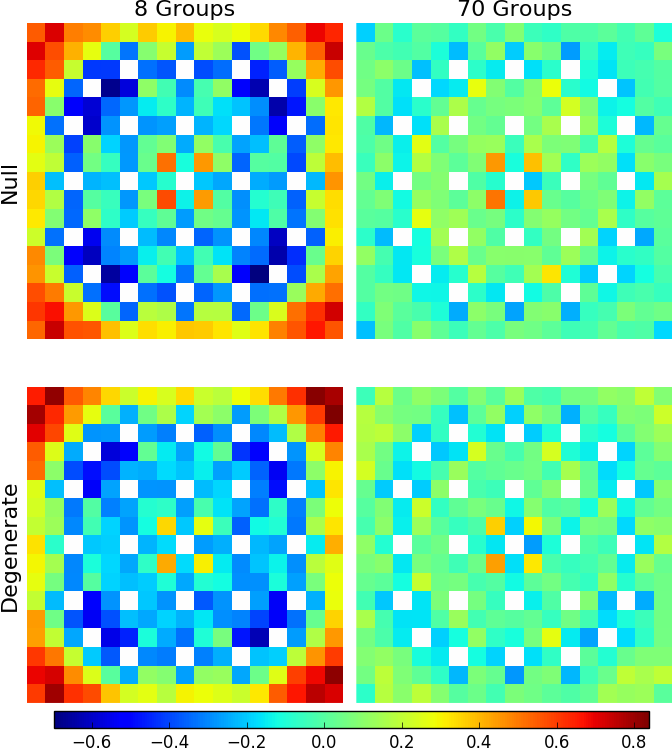
\includegraphics[width=\linewidth]{figures/quantification/assm-31/fiss-err}
\vspace{2mm}
\caption[Fission rate errors for a 3.1\% enriched assembly]{Fission rate percent relative errors for a 3.1\% enriched assembly corresponding to the reference in Fig.~\ref{fig:chap7-fiss-rates-3.1-assm}.}
\label{fig:chap8-assm-3.1-fiss-err}
\end{figure}

\clearpage

\begin{figure}[h!]
\centering
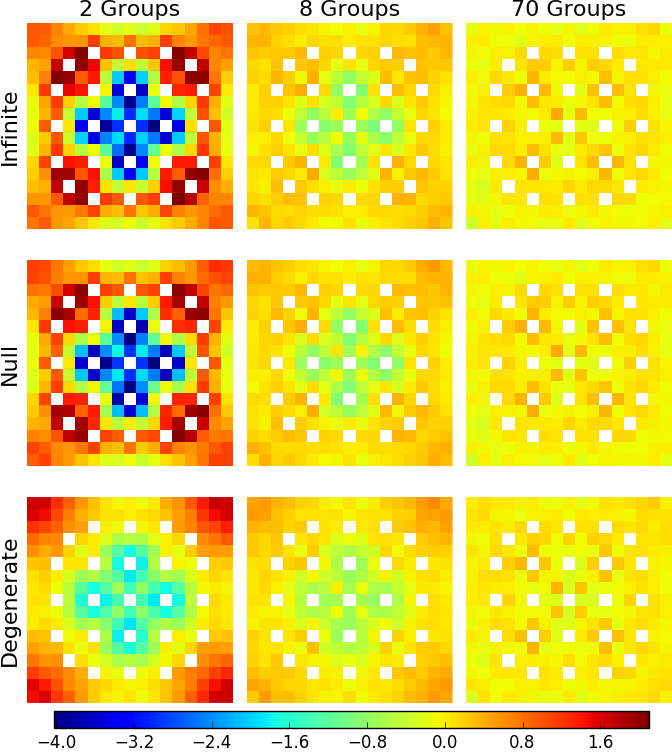
\includegraphics[width=\linewidth]{figures/quantification/assm-31-20BPs/fiss-err}
\vspace{2mm}
\caption[Fission rate errors for a 3.1\% enriched assembly with 20 BPs]{Fission rate percent relative errors for a 3.1\% enriched assembly with 20 BPs corresponding to the reference in Fig.~\ref{fig:chap7-fiss-rates-3.1-assm-20BAs}.}
\label{fig:chap8-assm-3.1-20BPs-fiss-err}
\end{figure}

\clearpage

\begin{figure}[h!]
\centering
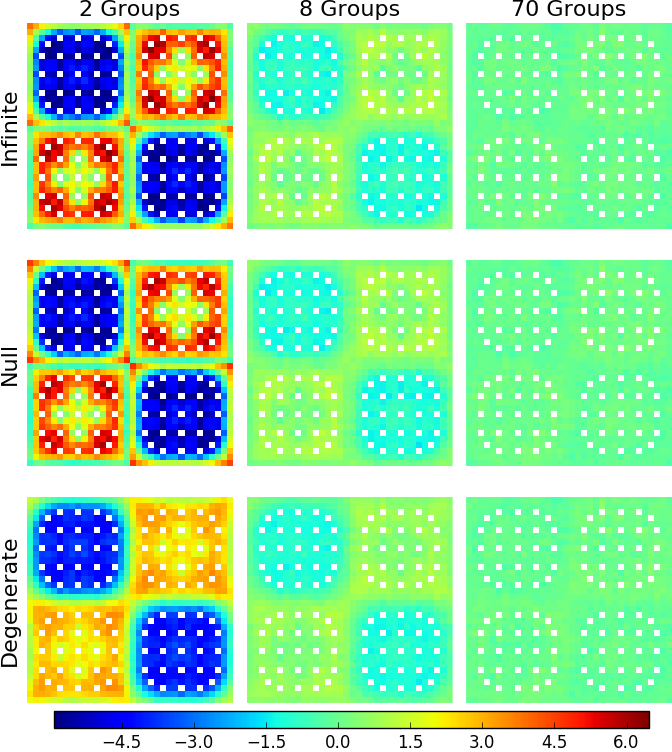
\includegraphics[width=\linewidth]{figures/quantification/2x2/fiss-err}
\vspace{2mm}
\caption[Fission rate errors for a 2$\times$2 colorset]{Fission rate percent relative errors for a 2$\times$2 colorset corresponding to the reference in Fig.~\ref{fig:chap7-fiss-rates-2x2}.}
\label{fig:chap8-2x2-fiss-err}
\end{figure}

\clearpage

\begin{figure}[h!]
\centering
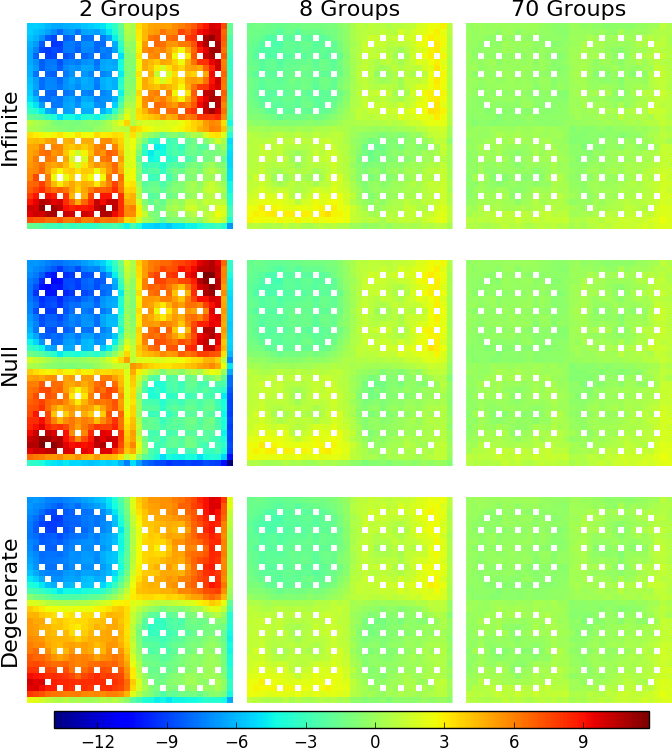
\includegraphics[width=\linewidth]{figures/quantification/reflector/fiss-err}
\vspace{2mm}
\caption[Fission rate errors for a 2$\times$2 colorset with a reflector]{Fission rate percent relative errors for a 2$\times$2 colorset with a reflector corresponding to the reference in Fig.~\ref{fig:chap7-fiss-rates-reflector}.}
\label{fig:chap8-reflector-fiss-err}
\end{figure}

\clearpage

\begin{figure}[h!]
\centering
\begin{subfigure}{\textwidth}
  \centering
  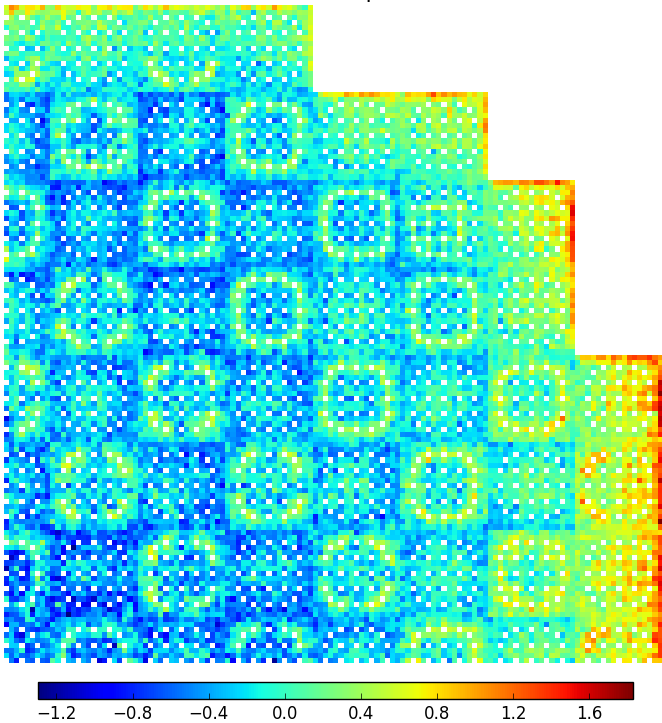
\includegraphics[width=0.6\linewidth]{figures/quantification/full-core/fiss-err-null}
  \caption{}
  \label{fig:chap8-full-core-fiss-err-null}
\end{subfigure}
\vspace{4mm}
\begin{subfigure}{\textwidth}
  \centering
  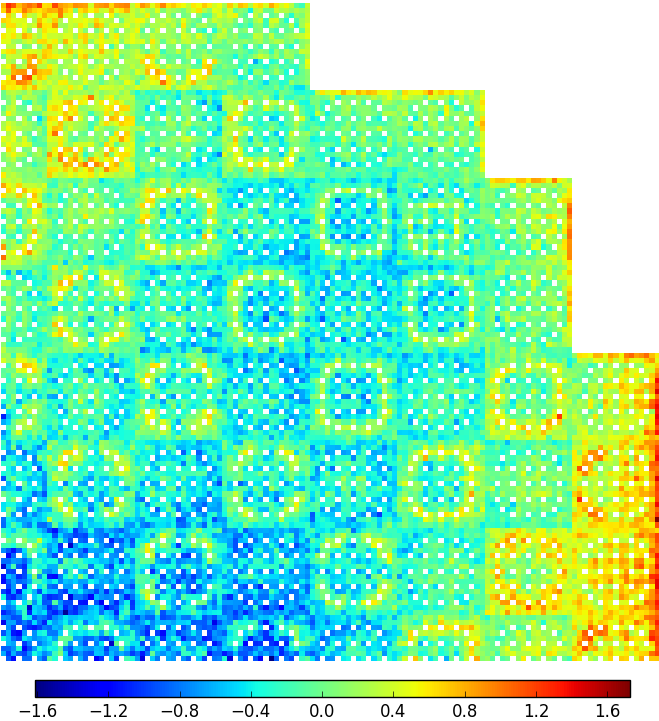
\includegraphics[width=0.6\linewidth]{figures/quantification/full-core/fiss-err-degenerate}
  \caption{}
  \label{fig:chap8-full-core-fiss-err-degenerate}
\end{subfigure}
\caption[Fission rate errors for the quarter core BEAVRS model]{Fission rate percent relative errors for the quarter core \ac{BEAVRS} model with null (a) and degenerate (b) homogenization corresponding to the reference in Fig.~\ref{fig:chap7-fiss-rates-reflector}.}
\label{fig:chap8-full-core-fiss-err}
\end{figure}

\clearpage


%%%%%%%%%%%%%%%%%%%%%%%%%%%%%%%%%%%%%%%%%%%%%
\subsection{U-238 Capture Rate Distributions}
\label{subsec:chap8-capt-rates}

The OpenMOC energy-integrated U-238 capture rates were compared to the reference OpenMC fission rates from Figs.~\Crefrange{fig:chap7-capt-rates-1.6-assm}{fig:chap7-capt-rates-full-core}. The percent relative errors for each pin's capture rates were computed and the maximum and mean errors are listed for each benchmark, energy group structure and spatial homogenization scheme in Tabs.~\ref{table:chap8-openmoc-max-capt-rates} and~\ref{table:chap8-openmoc-mean-capt-rates}, respectively. In particular, the maximum errors are the maximum of the absolute values of the errors along with the appropriate sign, while the mean errors are the averages of the absolute error magnitudes.

\vspace{0.1in}

\begin{table}[hb!]
  \centering
  \caption[Maximum OpenMOC U-238 capture rate errors]{Maximum absolute U-238 capture rate percent relative errors for varying spatial homogenization schemes and energy group structures.}
  \small
  \label{table:chap8-openmoc-max-capt-rates}
  \vspace{6pt}
  \begin{tabular}{l l R{2.5cm} R{2.5cm} R{2.5cm}}
  \toprule
  \rowcolor{lightgray}
  & & \multicolumn{3}{c}{\cellcolor{lightgray} \textbf{Max Error [\%]}} \\
  \multirow{-2}{*}{\cellcolor{lightgray} \bf Benchmark} &
  \multirow{-2}{*}{\cellcolor{lightgray} \bf \ac{MGXS} Scheme} &
  \multicolumn{1}{r}{{\cellcolor{lightgray} \bf 2-Group}} &
  \multicolumn{1}{r}{{\cellcolor{lightgray} \bf 8-Group}} &
  \multicolumn{1}{r}{{\cellcolor{lightgray} \bf 70-Group}} \\
  \midrule
\multirow{3}{*}{\parbox{2.5cm}{1.6\% Assm}} & Infinite & -2.644 & -1.480 & -1.102 \\
& Null & -2.629 & -1.475 & -1.101 \\
& Degenerate & 1.075 & 0.484 & 0.386 \\
  \midrule
\multirow{3}{*}{\parbox{2.5cm}{3.1\% Assm}} & Infinite & -2.959 & -1.678 & -1.262 \\
& Null & -2.934 & -1.670 & -1.262 \\
& Degenerate & 0.941 & 0.437 & 0.326 \\
  \midrule
\multirow{3}{*}{\parbox{2.5cm}{3.1\% Assm w/ 20 BPs}} & Infinite & 3.245 & -1.278 & -0.978 \\
& Null & 3.193 & -1.253 & -0.946 \\
& Degenerate & 1.635 & 0.571 & 0.311 \\
  \midrule
\multirow{3}{*}{\parbox{2.5cm}{2$\times$2 Colorset}} & Infinite & -5.001 & -1.743 & -1.307 \\
& Null & -4.591 & -1.598 & -1.305 \\
& Degenerate & -2.983 & -0.954 & 0.615 \\
  \midrule
\multirow{3}{*}{\parbox{2.5cm}{2$\times$2 Colorset w/ Reflector}} & Infinite & 12.010 & 3.618 & -1.889 \\
& Null & 11.100 & 3.372 & -1.969 \\
& Degenerate & 8.260 & 2.787 & -0.783 \\
  \midrule
\multirow{3}{*}{\parbox{2.5cm}{BEAVRS Quarter Core}} & Infinite & -79.033 & -31.419 & -3.655 \\
& Null & -84.954 & -31.773 & -3.645 \\
& Degenerate & -84.624 & -31.392 & -2.067 \\
  \bottomrule
\end{tabular}
\end{table}

\begin{table}[h!]
  \centering
  \caption[Mean OpenMOC U-238 capture rate errors]{Mean absolute U-238 capture rate percent relative errors for varying spatial homogenization schemes and energy group structures.}
  \small
  \label{table:chap8-openmoc-mean-capt-rates}
  \vspace{6pt}
  \begin{tabular}{l l R{2.5cm} R{2.5cm} R{2.5cm}}
  \toprule
  \rowcolor{lightgray}
  & & \multicolumn{3}{c}{\cellcolor{lightgray} \textbf{Mean Error [\%]}} \\
  \multirow{-2}{*}{\cellcolor{lightgray} \bf Benchmark} &
  \multirow{-2}{*}{\cellcolor{lightgray} \bf \ac{MGXS} Scheme} &
  \multicolumn{1}{r}{{\cellcolor{lightgray} \bf 2-Group}} &
  \multicolumn{1}{r}{{\cellcolor{lightgray} \bf 8-Group}} &
  \multicolumn{1}{r}{{\cellcolor{lightgray} \bf 70-Group}} \\
  \midrule
\multirow{3}{*}{\parbox{2.5cm}{1.6\% Assm}} & Infinite & 1.252 & 0.643 & 0.480 \\
& Null & 1.247 & 0.641 & 0.479 \\
& Degenerate & 0.367 & 0.091 & 0.086 \\
  \midrule
\multirow{3}{*}{\parbox{2.5cm}{3.1\% Assm}} & Infinite & 1.371 & 0.718 & 0.543 \\
& Null & 1.361 & 0.715 & 0.543 \\
& Degenerate & 0.326 & 0.106 & 0.087 \\
  \midrule
\multirow{3}{*}{\parbox{2.5cm}{3.1\% Assm w/ 20 BPs}} & Infinite & 1.278 & 0.551 & 0.424 \\
& Null & 1.261 & 0.543 & 0.414 \\
& Degenerate & 0.443 & 0.150 & 0.089 \\
  \midrule
\multirow{3}{*}{\parbox{2.5cm}{2$\times$2 Colorset}} & Infinite & 2.300 & 0.611 & 0.451 \\
& Null & 2.007 & 0.616 & 0.446 \\
& Degenerate & 1.482 & 0.170 & 0.154 \\
  \midrule
\multirow{3}{*}{\parbox{2.5cm}{2$\times$2 Colorset w/ Reflector}} & Infinite & 3.878 & 0.847 & 0.480 \\
& Null & 3.708 & 0.780 & 0.478 \\
& Degenerate & 3.302 & 0.655 & 0.165 \\
  \midrule
\multirow{3}{*}{\parbox{2.5cm}{BEAVRS Quarter Core}} & Infinite & 34.706 & 10.005 & 0.556 \\
& Null & 39.137 & 10.164 & 0.474 \\
& Degenerate & 39.370 & 10.137 & 0.345 \\
  \bottomrule
\end{tabular}
\end{table}

As was the case for the other metrics, the U-238 capture rate errors are highly dependent on energy group structure. The maximum and mean errors are substantially reduced with finer energy group structures for all benchmarks and spatial homogenization schemes. The maximum capture rate errors are 2 -- 12\% in 2 groups for the individual fuel assembly and 2$\times$2 colorset benchmarks, respectively, but decrease to 0.4 -- 1.7\% when modeled with 70 groups. The mean capture rate errors likewise decrease with finer energy group structures, and are less than 0.6\% in magnitude for the assembly and colorset benchmarks for all homogenization schemes with 70 groups.

The capture rate errors are more dependent on the spatial homogenization scheme used to compute \ac{MGXS} in the fuel than are the fission rate errors. In particular, the degenerate scheme produces much smaller maximum and mean errors than the null and infinite schemes. The maximum error is greater than 1\% for all benchmarks with the infinite and null schemes even with 70 energy groups. The maximum error is reduced by 2 -- 5$\times$ for all benchmarks with the use of degenerate homogenization. In addition, the degenerate scheme consistently reduces the error for all energy group structures, with the most substantial improvement over the infinite and null schemes observed for 70 groups. This stands in contrast to the fission rate errors where the degenerate scheme was only significantly better for 2-group \ac{MGXS}. As was the case for the fission rate errors, the null and infinite schemes exhibit a negligible difference in their maximum and mean capture rate errors, with no systematic trend in the data.

The spatial distributions of capture rate errors are plotted as heatmaps for each benchmark in Figs.~\Crefrange{fig:chap8-assm-1.6-capt-err}{fig:chap8-full-core-capt-err}. These figures illustrate the capture rate errors for 8 and 70 energy group structures for the null and degenerate schemes; the capture rate errors for 2, 8, and 70 groups for all three homogenization schemes are compared in Figs.~\Crefrange{fig:quantify-assm-1.6-capt-err}{fig:quantify-full-core-capt-err} in App.~\ref{sec:quantify-capt-rates}. In addition, the U-238 capture absolute errors for the benchmarks with vacuum \acp{BC} are illustrated in Figs.~\ref{fig:quantify-reflector-capt-err-abs} and~\ref{fig:quantify-full-core-capt-err-abs} in App.~\ref{sec:quantify-capt-rates-absolute}.

The heatmaps illustrate systematic error trends in the pin-wise capture errors which correlate with spatial heterogeneities in each benchmark. As is observed for the fission rates, the capture rates are generally underpredicted for pins near \acp{CRGT}, but overpredicted for pins removed from \acp{CRGT}, such as those in the corners of the fuel assembly. Unlike the fission rates, the capture rates are also underpredicted for pins near \acp{BP}. The effects due to heterogeneities are further enhanced when differentiating pins which are facially adjacent to \acp{CRGT}, facially and corner adjacent to two \acp{CRGT}, etc. In addition, the error magnitudes are large for pins along the inter-assembly and assembly-reflector interfaces for the 2$\times$2 colorset benchmarks. For the \ac{PWR} benchmarks modeled here, the differential moderation provided by neighboring \acp{CRGT} and/or reflectors softens the local flux for nearby fuel pins and should be modeled when collapsing pin-wise \ac{MGXS} for high-fidelity multi-group transport calculations.

\begin{figure}[h!]
\centering
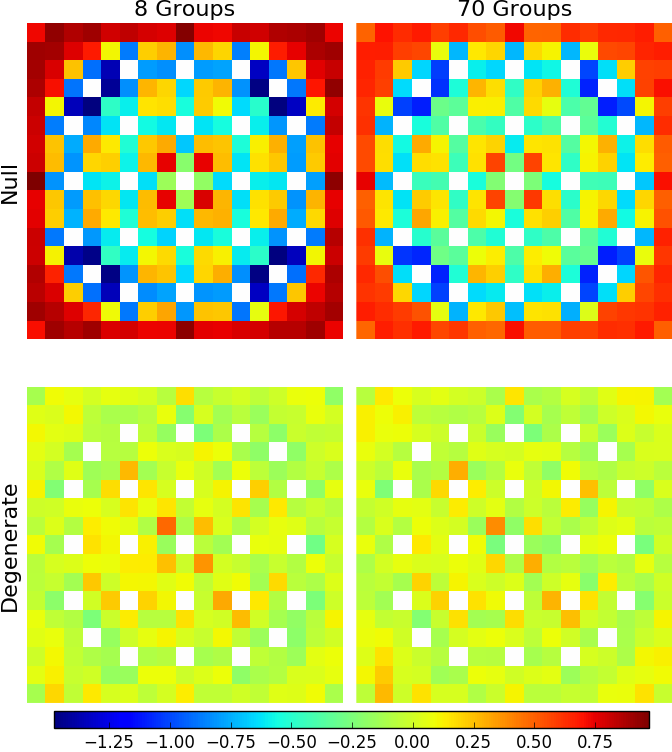
\includegraphics[width=\linewidth]{figures/quantification/assm-16/capt-err}
\vspace{2mm}
\caption[U-238 capture rate errors for a 1.6\% enriched assembly]{U-238 capture rate percent relative errors errors for a 1.6\% enriched assembly corresponding to the reference in Fig.~\ref{fig:chap7-capt-rates-1.6-assm}.}
\label{fig:chap8-assm-1.6-capt-err}
\end{figure}

\clearpage

\begin{figure}[h!]
\centering
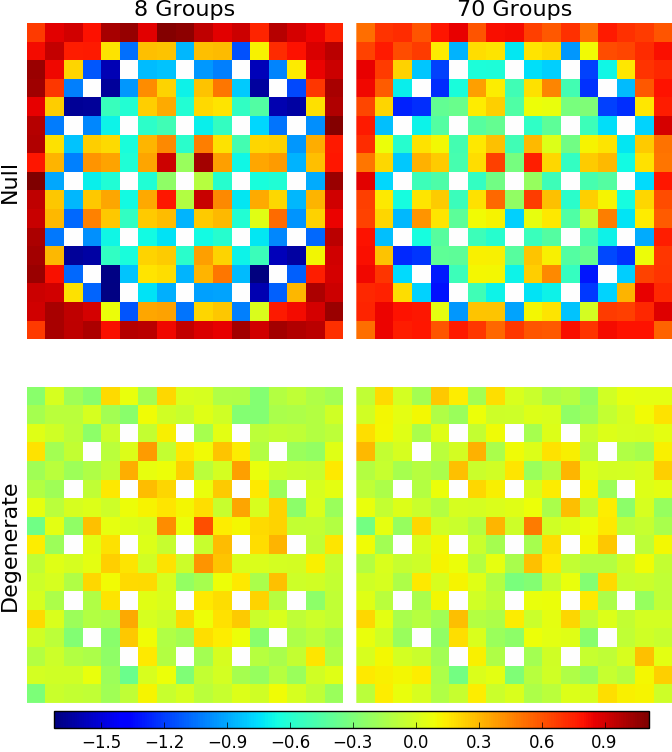
\includegraphics[width=\linewidth]{figures/quantification/assm-31/capt-err}
\vspace{2mm}
\caption[U-238 capture rate errors for a 3.1\% enriched assembly]{U-238 capture rate percent relative errors errors for a 3.1\% enriched assembly corresponding to the reference in Fig.~\ref{fig:chap7-capt-rates-3.1-assm}.}
\label{fig:chap8-assm-3.1-capt-err}
\end{figure}

\clearpage

\begin{figure}[h!]
\centering
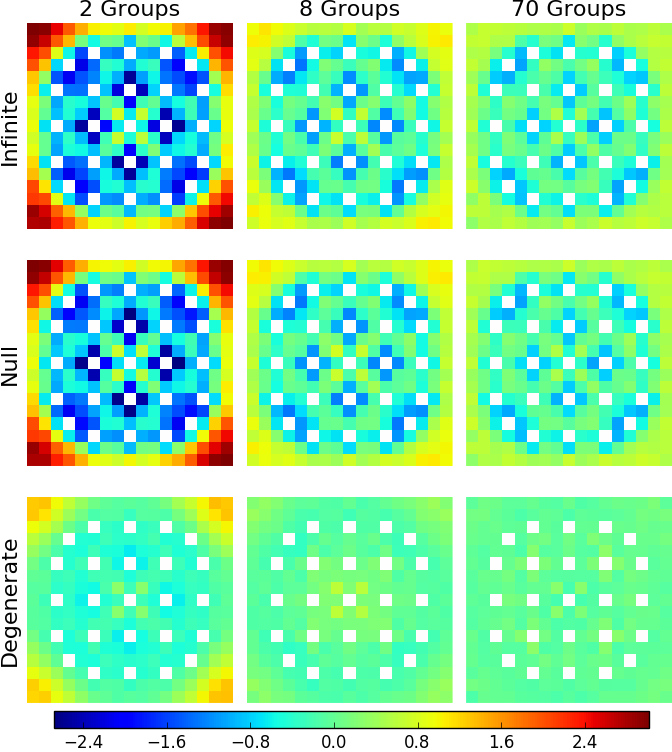
\includegraphics[width=\linewidth]{figures/quantification/assm-31-20BPs/capt-err}
\vspace{2mm}
\caption[U-238 capture rate errors for a 3.1\% enriched assembly with 20 BPs]{U-238 capture rate percent relative errors errors for a 3.1\% enriched assembly with 20 \acp{BP} corresponding to the reference in Fig.~\ref{fig:chap7-capt-rates-3.1-assm-20BAs}.}
\label{fig:chap8-assm-3.1-20BPs-capt-err}
\end{figure}

\clearpage

\begin{figure}[h!]
\centering
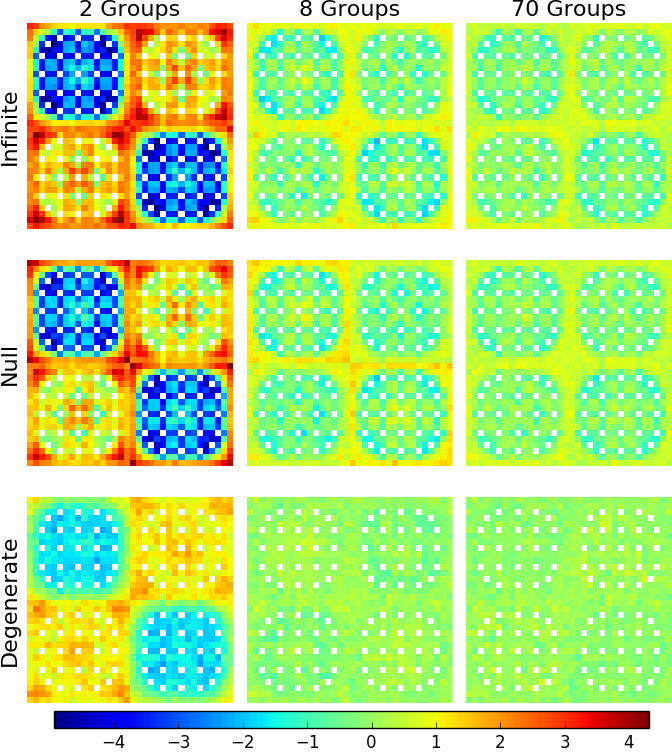
\includegraphics[width=\linewidth]{figures/quantification/2x2/capt-err}
\vspace{2mm}
\caption[U-238 capture rate errors for a 2$\times$2 colorset]{U-238 capture rate percent relative errors errors for a 2$\times$2 colorset corresponding to the reference in Fig.~\ref{fig:chap7-capt-rates-2x2}.}
\label{fig:chap8-2x2-capt-err}
\end{figure}

\clearpage

\begin{figure}[h!]
\centering
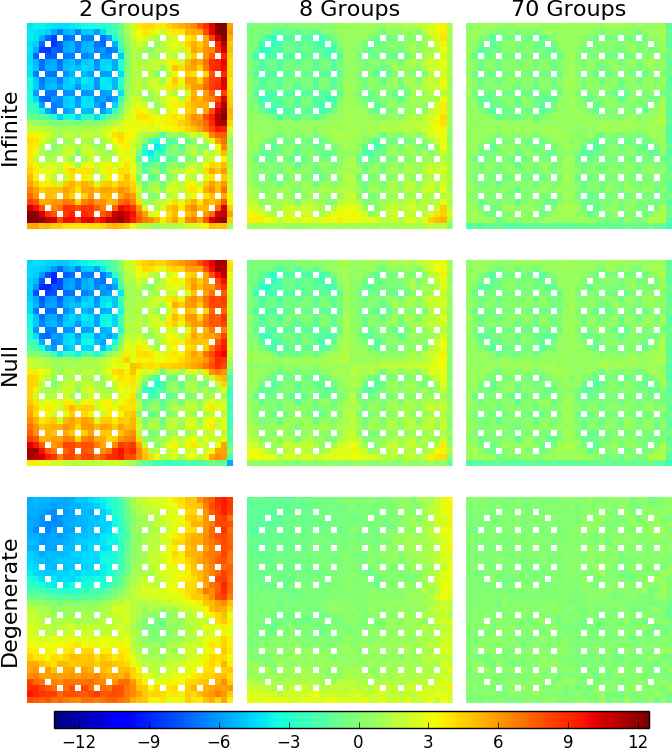
\includegraphics[width=\linewidth]{figures/quantification/reflector/capt-err}
\vspace{2mm}
\caption[U-238 capture rate errors for a 2$\times$2 colorset with a reflector]{U-238 capture percent relative errors rate errors for a 2$\times$2 colorset with a reflector corresponding to the reference in Fig.~\ref{fig:chap7-capt-rates-reflector}.}
\label{fig:chap8-reflector-capt-err}
\end{figure}

\clearpage

\begin{figure}[h!]
\centering
\begin{subfigure}{\textwidth}
  \centering
  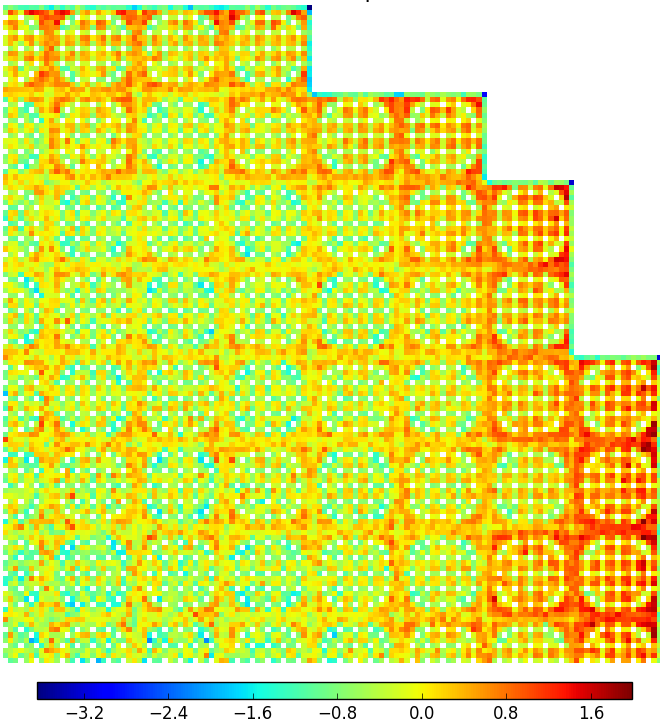
\includegraphics[width=0.6\linewidth]{figures/quantification/full-core/capt-err-null}
  \caption{}
  \label{fig:chap8-full-core-capt-err-null}
\end{subfigure}
\vspace{4mm}
\begin{subfigure}{\textwidth}
  \centering
  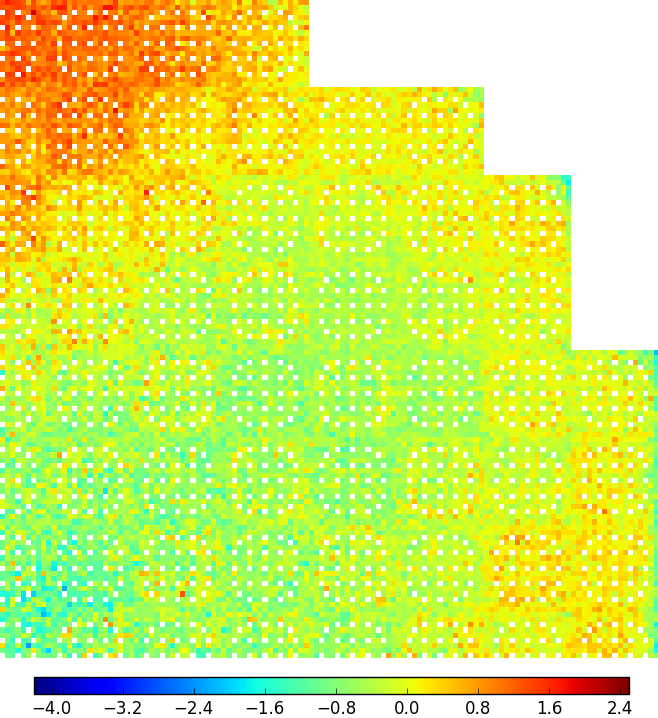
\includegraphics[width=0.6\linewidth]{figures/quantification/full-core/capt-err-degenerate}
  \caption{}
  \label{fig:chap8-full-core-capt-err-degenerate}
\end{subfigure}
\caption[U-238 capture rate errors for the quarter core \ac{BEAVRS} model]{U-238 capture rate percent relative errors for the quarter core \ac{BEAVRS} model with null (a) and degenerate (b) homogenization corresponding to the reference in Fig.~\ref{fig:chap7-capt-rates-full-core}.}
\label{fig:chap8-full-core-capt-err}
\end{figure}

\clearpage

As noted previously, the energy group structure has a large impact on the error distributions as can be seen from the figures. In addition, the heatmaps illustrate how the degenerate spatial homogenization scheme effectively ``smooths'' the pin-wise errors as compared to the infinite and null schemes. Although this effect appears most pronounced for the 2-group plots in App.~\ref{sec:quantify-capt-rates}, the ``smoothing'' trend persists for 8 and 70 groups as well (unlike the fission rate errors). In particular, the differential of the errors for pins near \acp{CRGT}, \acp{BP}, and assembly and reflector interfaces is substantially reduced when degenerate homogenization is applied. The difference in the spatial distributions of errors for the infinite and null schemes is hardly noticeable except for pins near the assembly and reflector interfaces for the 2$\times$2 colorset benchmarks.

\begin{emphbox}
\textbf{The use of degenerate spatial homogenization ``smooths'' the spatial distribution of pin-wise U-238 capture rate errors. The improvement in accuracy with degenerate homogenization increases with more energy groups. This underscores the importance of accounting for spatial heterogeneities -- such as the differential moderation from \acp{CRGT} and reflectors -- when generating \ac{MGXS} to predict U-238 capture and Pu-239 production in \acp{LWR}.}
\end{emphbox}


%%%%%%%%%%%%%%%%%%%%%%%%%%%%%%%%%%%%%%%%%%%%%%%%%%%%%%%%%%%%%%%%%%%%%%%%%%%%%%%
\section{Motivation for a New Spatial Homogenization Scheme}
\label{sec:chap8-motivate}

The results presented in the preceding section quantify and illustrate the impact of capturing heterogeneous spatial self-shielding effects in \ac{MGXS} for fuel pins in \ac{PWR} geometries. The pin-wise U-238 capture rates, and to a lesser extent, the pin-wise fission rates, are better predicted when these effects are incorporated into \ac{MGXS} used in high-fidelity multi-group transport calculations. Alternatively, non-negligible systematic approximation errors in the reaction rates arise when using \ac{MGXS} collapsed with the flux from an infinite lattice calculation which does not differentiate pins based on neighboring spatial heterogeneities\footnote{This is the case for many traditional approaches to self-shielding for \ac{MGXS} generation.}. It should be noted that other approximation errors due to spatial, angular and energy discretization in \ac{MOC} are still present in these calculations, and may complicate the generality of the conclusions drawn in this section.

The use of degenerate spatial homogenization reduces reaction rate errors by directly modeling perturbations in the flux within each fuel pin due to local heterogeneities such as neighboring \acp{CRGT} and \acp{BP}. Some reactions may be more or less sensitive to local spatial self-shielding effects. In the \ac{PWR} benchmarks presented here, degenerate homogenization was most beneficial for predicting U-238 capture rates since it explicitly accounts for differential moderation from neighboring \acp{CRGT} and reflectors. Although degenerate spatial homogenization is advantageous for accuracy, it is not practical for routine reactor analysis due to computational resource limitations.

As shown in Tab.~\ref{table:chap8-num-materials}, the number of unique materials in the \ac{BEAVRS} model is $\mathcal{O}(10^{4})$ for degenerate homogenization\footnote{The number of materials may be $\mathcal{O}(10^{6})$ for 3D \ac{PWR} models with axial enrichment zoning.}, but only $\mathcal{O}(10)$ for the infinite and null homogenization schemes. As a result of the fine-grained spatial tally mesh employed by degenerate homogenization, far more particle histories are needed to converge the \ac{MGXS} tallies to obtain the same statistical uncertainties as with the simpler schemes. In particular, the particle track density across each of the degenerate tally zones (\textit{e.g}, fuel pins) is roughly one ten thousandth of that in the infinite/null schemes. Therefore, a factor of roughly 10,000 more particle histories are required to obtain the same particle track density within each of the degenerate tally zones\footnote{For eigenvalue calculations in high dominance ratio reactor cores, the additional number of particle histories needed to converge \ac{MGXS} tallies for degenerate homogenization may be even greater due to the highly uneven fission neutron source distribution.} and converge the statistical uncertainties to the same level as would be obtained with infinite/null homogenization.

However, the  spatial distribution of errors motivate the potential for a new homogenization scheme. In particular, the errors in the infinite/null homogenization schemes exhibit marked patterns which correlate with the local heterogeneities in the geometry. For example, the error of the predicted reaction rates for all pins facially adjacent to a \ac{CRGT} is quite similar. More generally, the observed reaction rate errors are similar for groups of pins with similar neighboring local heterogeneities. This key observation implies that the reaction rate errors may be minimized if an appropriate set of spatially self-shielded \ac{MGXS} are defined for each grouping of pins with similar flux profiles due to neighboring heterogeneities. In particular, can a library of \ac{MGXS} be homogenized across a greatly reduced set of pins from the degenerate case which approaches both:

\begin{itemize}[noitemsep]
\item the \textbf{accuracy} of the degenerate scheme
\item the \textbf{convergence} of the infinite/null schemes
\end{itemize}

\noindent with far fewer particle histories than the degenerate scheme? This question is investigated with an in-depth analysis of clustering of pin-wise \ac{MGXS} in the following chapter.

%\begin{itemize}[noitemsep]
%  \item Plot evolution of rel. err. by batch for each homogenization scheme
%  \begin{itemize}[noitemsep]
%    \item groups with highest rel. err.
%    \item reactions with greatest contribution to eigenvalue (U-238 capture)
%    \item total (track-length) vs. scattering matrices (analog)    
%    \item which group structure(s)?
% \end{itemize}
%  \item compare to pin power convergence rates in preceding chapter
%\end{itemize}

%-infinite vs. null vs. degenerate
%-conv rates for MGXS in each case - choose worst groups
%  -compare back to pin power error conv. rates
%  -convergence rates for infinite vs. null vs. degenerate

\clearpage

\vfill
\begin{highlightsbox}[frametitle=Highlights]
\begin{itemize}
  \item Each of the six heterogeneous benchmarks introduced in Chap.~\ref{chap:benchmarks} is modeled in OpenMOC with \ac{MGXS} generated by OpenMC.
  \item Three spatial homogenization schemes enable a direct quantification of spatial self-shielding effects from local heterogeneities in \ac{MGXS}:
  \begin{itemize}
    \item \textbf{\textit{Infinite homogenization}} tallies \ac{MGXS} for each unique fuel pin type using the \ac{MC} flux in an infinite lattice calculation.
    \item \textbf{\textit{Null homogenization}} tallies \ac{MGXS} for each unique fuel pin type using the \ac{MC} flux from the complete heterogeneous geometry.
    \item \textbf{\textit{Degenerate homogenization}} tallies \ac{MGXS} for each unique fuel pin instance using the \ac{MC} flux from the complete heterogeneous geometry.
  \end{itemize}
  \item The OpenMOC eigenvalues match OpenMC to within nearly 250 \ac{pcm} for all benchmarks and homogenization schemes with 70-group \ac{MGXS}.
  \item Degenerate homogenization best predicts reaction rates most sensitive to spatial self-shielding since it incorporates perturbations to the flux due to heterogeneities such as \acp{CRGT} and \acp{BP}.
  \begin{itemize}
    \item Fission rate errors do not improve significantly
    \item \textbf{U-238 capture rate errors are reduced by 2 -- 4$\times$}
  \end{itemize}
  \item Degenerate homogenization requires far more particle histories to converge \ac{MC} \ac{MGXS} tallies than the simpler infinite and null schemes.
  \item The pin-wise reaction rate error distributions motivate the development of a new spatial homogenization scheme to identify groups of fuel pins which experience similar spatial self-shielding effects and have similar \ac{MGXS}.
\end{itemize}
\end{highlightsbox}
\vfill